% https://www.overleaf.com/latex/templates/sprint-beyond-the-book-template/kgckkccxfxcj
% 這份報告是用上面網址裡的資料建立的

\documentclass[nols]{tufte-book}
%\documentclass{tufte-handout}
\usepackage[caption=false]{subfig}

\usepackage{booksprint}

\setcounter{secnumdepth}{3}
\setcounter{tocdepth}{1}

\usepackage{pdfpages}


\usepackage{fancyhdr}
% 加上 table in the header 
% https://tex.stackexchange.com/questions/113240/tables-as-header-and-footer

% 設定頁碼樣式
\fancypagestyle{plain}{%
  \fancyhf{}
  \fancyfoot[C]{\thepage}
  \renewcommand{\headrulewidth}{0pt}
  \renewcommand{\footrulewidth}{0pt}
}
\fancyfoot[C]{\normalfont\small\thepage}


\usepackage{hyperref} %加入 hyperlink

\usepackage{natbib}

%\usepackage[utf8]{inputenc}
\usepackage[T1]{fontenc}
\usepackage{fontspec}
\renewcommand{\allcapsspacing}[1]{{\addfontfeature{LetterSpace=10.0}#1}}
\renewcommand{\smallcapsspacing}[1]{{\addfontfeature{LetterSpace=5.0}#1}}
\renewcommand{\textsc}[1]{\smallcapsspacing{\textsmallcaps{#1}}}
\renewcommand{\smallcaps}[1]{\smallcapsspacing{\scshape\MakeTextLowercase{#1}}}
% https://www.overleaf.com/latex/examples/demonstration-of-noto-serif-cjk-and-noto-sans-cjk-fonts/sgrwgcddtqsq
\usepackage{setspace}


%set-up 中文環境
\usepackage[CJKspace]{xeCJK}
\usepackage{xpinyin}

\setmainfont{Noto Serif Light}
\setsansfont{Noto Sans}
\setmonofont[Scale=MatchLowercase]{Noto Mono}

\setCJKmainfont{Noto Serif CJK TC}
\setCJKsansfont{Noto Sans CJK TC}
\setCJKmonofont{Noto Sans Mono CJK TC}


%表格
\usepackage{amsmath}
\usepackage{amssymb}
\usepackage{hyperref}
\usepackage{array}

\usepackage{tabularx}
\usepackage{multirow}

\usepackage{ragged2e}
\usepackage{longtable}

\begin{document}
%\pagenumbering{roman}


\title[Structural Heart Disease Intervention]{
\logos
\textbf{經導管心臟瓣膜治療技術\\
Transcatheter Valve\\ Intervention\\
新竹臺大分院心血管中心 \\ 
出國進修計畫成果報告- 附錄}}
\author{謝慕揚醫師, Drake, Mu-Yang Hsieh,MD, PhD}
\date{\today}


\tableofcontents

\onehalfspacing



\chapter{TEER}
% https://www.acc.org/Latest-in-Cardiology/Articles/2022/07/29/17/19/Pre-Procedural-Interventional-TEE-Tricuspid-Valve

% https://www.sciencedirect.com/science/article/pii/S2772374723001783
% technical history: Feldman2009

二尖瓣逆流（Mitral Regurgitation, MR）是最常見的瓣膜性心臟病，若未治療，將導致生活品質下降、心臟衰竭（Heart Failure, HF）及死亡率增加。自2008年在歐洲開展以來，經導管二尖瓣緣對緣修復技術（Mitral Valve Transcatheter Edge-to-Edge Repair, M-TEER）已逐漸成為非手術治療重度且有症狀MR患者的重要策略。

二尖瓣返流（Mitral Regurgitation, MR）是最常見的瓣膜性心臟病，影響了約10\%以上75歲以上的人群。
歐洲研究顯示，約50\%的重度症狀性MR患者因年齡大、左心室功能受損及合併症多而未接受外科手術，顯示出開發微創治療的必要性。\cite{Puls2016}

MitraClip是一種經皮的二尖瓣修復技術，基於Alfieri提出的外科技術，於2003年首次應用於動物模型及人類，並經 Dr. Feldman 發展。
該技術在EVEREST I試驗中被證明是安全和可行的，隨後的EVEREST II試驗比較了經皮修復與外科手術，發現經皮修復安全性更高，但部分患者需在12個月內接受額外的手術干預。\cite{Feldman2005}

隨著器械及手術技術的進步，M-TEER在歐洲與美國guideline中獲得推薦。本文將包含M-TEER的review與整理Mainz具體作法，包括術前患者評估、器械選擇、手術導引及後續管理，並討論原發性（Primary Mitral Regurgitation, PMR）與繼發性（Secondary Mitral Regurgitation, SMR）MR的治療證據。


\section{Background}
二尖瓣逆流（Mitral Regurgitation, MR）是一種高度盛行的疾病，大約10\%的75歲及以上人群患有臨床相關的MR\cite{Hausleiter2023, Hausleiter2023a}.若未進行治療，重度MR可能導致左心室功能不全、心輸出量減少及肺充血，進而引發心衰竭（Heart Failure, HF）症狀、生活品質下降及死亡率增加.\cite{Goel2014} 許多重度MR患者因手術風險增加或無法進行手術而未得到充分治療，因此發展了經導管治療以應對這部分患者的需求。\cite{Nkomo2006}

% 注意: 2003應該只有在之豬身上作動物實驗吧?

自2003年首次在人類臨床應用二尖瓣經導管緣對緣修復（Mitral Valve Transcatheter Edge-to-Edge Repair, M-TEER）技術以來，該技術於2008年獲得歐盟CE（European Conformity）認證，並分別於2013年和2019年獲得美國食品藥品監督管理局（FDA）對原發性MR（Primary MR, PMR）和繼發性MR（Secondary MR, SMR）的批准。

目前臺灣地區新竹臺大分院，依2023年建立的超音波資料庫，每個月均有2-8人被診斷有中至重度或重度的MR. 其中有部份病人有許多共病而無法接受外科手術治療。

Only 5.6\% of patients who underwent isolated MV surgery in the Society of Thoracic Surgeons (STS) database from 2008 to 2012 had an STS-predicted mortality rate of >12\% (response to a query of the STS database conducted in December 2012 of all isolated MV surgeries between 2008 and 2012).\cite{Glower2014}

\marginnote{\textbf{STS score > 12\% 為許多trials裡面的high-risk patient definition.}}

\newpage
\section{2024 Update of Trials}
\begin{figure}
    \centering
    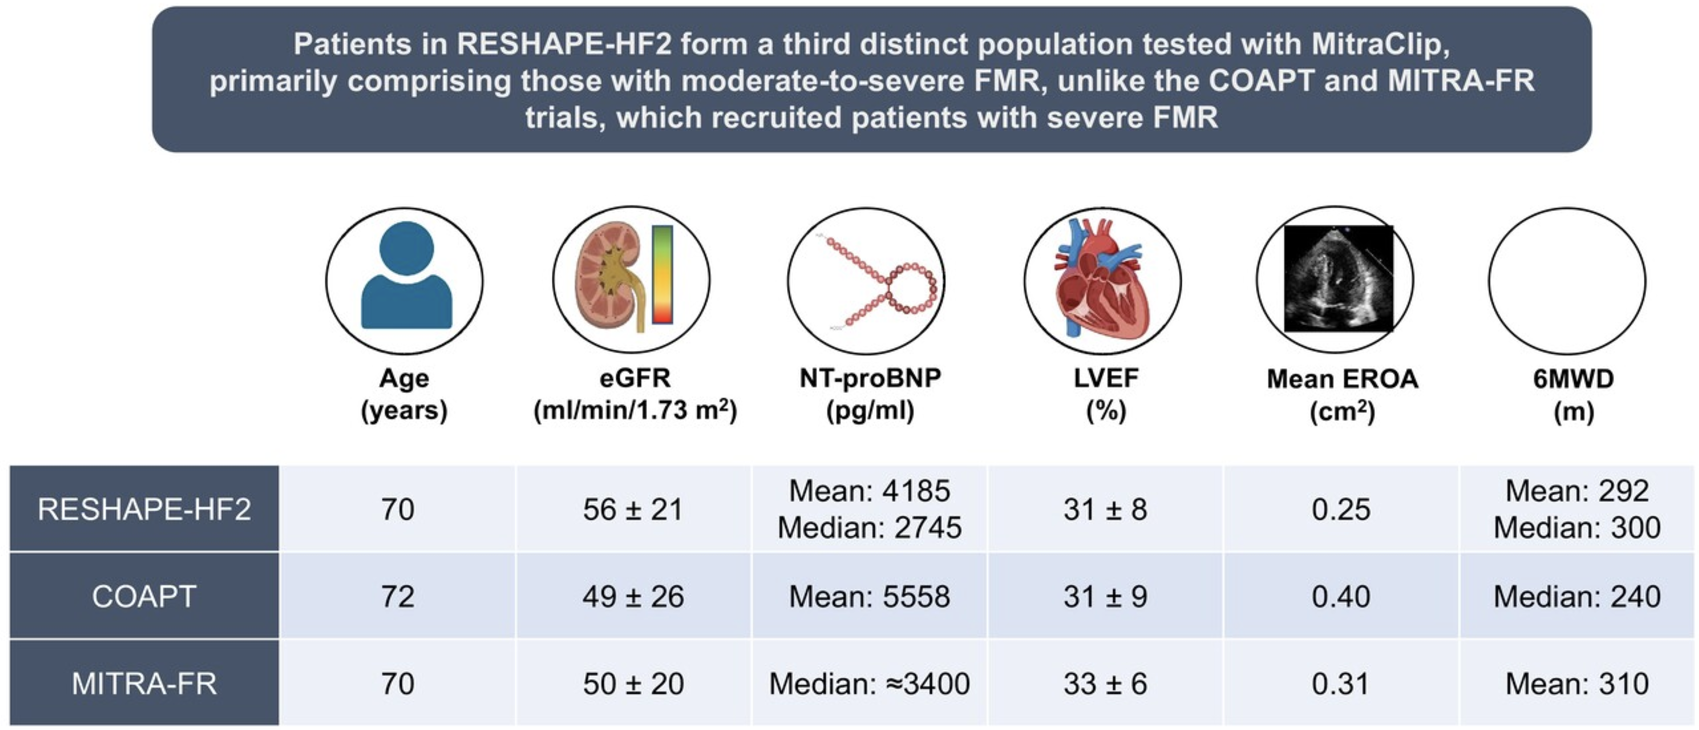
\includegraphics[width=1\linewidth]{images/teer/fig COAPT Matterhorn RESHAPE HF2.png}
    \caption{2024為止重要trials的整理: COAPT, Matterhorn, RESHAPE-HF2. }
    \label{COAPT Matterhorn RESHAPE HF2}
\end{figure}

COAPT (2018): COAPT 試驗（心血管結果評估 MitraClip 經皮治療功能性二尖瓣逆流心衰竭患者）於 2018 年發表。這項具有里程碑意義的研究旨在評估 MitraClip 裝置在有症狀的心衰竭患者中對嚴重功能性二尖瓣逆流（MR）的安全性和有效性。參與者被隨機分配接受 MitraClip 加上指導下的最佳藥物治療（GDMT）或僅接受 GDMT。研究結果顯示，MitraClip 顯著減少了心衰竭住院次數，並改善了生存率，相較於僅接受 GDMT 的患者。該試驗的結果促使美國 FDA 在 2019 年批准擴大 MitraClip 的適應症，確認其在治療嚴重心衰竭患者中的作用。\cite{Stone2018, Tachibana2023}

MITRA-FR (2019): MITRA-FR 試驗於 2019 年發表，聚焦於相似的患者群體，但與 COAPT 的結果有所不同。這項試驗同樣評估了 MitraClip 裝置在功能性二尖瓣逆流患者中的效果，但發現與最佳藥物治療相比，並未顯示出顯著降低死亡率或住院率。不同的結果引發了對患者選擇和 MR 嚴重程度的質疑，建議 MITRA-FR 可能招募了左心室擴大的更嚴重患者，這可能影響了其結果。\cite{Obadia2018}

RESHAPE-HF2 (2024): RESHAPE-HF2 試驗於 2024 年 9 月報告結果，旨在評估 MitraClip 在中度至嚴重功能性二尖瓣逆流患者中的有效性。該試驗發現，MitraClip 治療在多個主要終點上優於最佳藥物治療，包括死亡和心衰竭住院的綜合指標。然而，與 COAPT 相比，RESHAPE-HF2 並未顯示出顯著降低全因死亡率。這些結果被認為支持 COAPT 的研究結果，表明即使在較輕度 MR 案例中，MitraClip 也可能是有益的。\cite{Anker2024}

MATTERHORN 試驗 (2024): MATTERHORN 試驗於 2024 年發表，這是首個隨機對照試驗直接比較經導管邊緣對邊緣修復（TEER）與手術在高風險二尖瓣逆流患者中的效果。該研究招募了 210 名高風險手術患者（平均年齡 75 歲；40\% 為女性），其左心室射血分數 ≥20\%，並在最佳藥物治療下仍有心衰竭症狀。參與者被隨機分為 TEER 組或手術組。結果顯示，在主要綜合終點（包括死亡、心衰竭住院、二尖瓣再介入、輔助裝置植入及中風）方面，TEER 組為 16.7\%，手術組為 22.5\%，符合非劣效性標準（p<0.01）。此外，TEER 組的安全性明顯優於手術組，主要安全終點事件發生率分別為 14.9\% 和 54.8\%。這些結果顯示 TEER 在高風險二尖瓣逆流患者中是一個可行的治療選擇。\cite{Baldus2024}

\section{MR and TR evaluation}



\subsection{Clinical evaluation}

臨床評估包括進行身體檢查以尋找心衰竭（Heart Failure, HF）的徵象，並根據紐約心臟病學會（New York Heart Association, NYHA）分類對症狀狀態進行分級。病患之前的病史，共病，與過去的心衰竭住院歷程，都會改變治療決策，病患的肝功能與腎功能也同樣重要。\cite{Tachibana2023}

應評估患者的生活品質，最好使用標準化的心衰竭（Heart Failure, HF）問卷進行評估。目前研究用標準化的心衰問卷為: Kansas City Cardiomyopathy Questionnaire (KCCQ) (Table ~\ref{table KCCQ}). 另外再加上客觀的評估依據 (Table ~\ref{table objective evaluation}) 與心臟超音波檢查。

在心臟超音波檢查後，另應有冠狀動脈相關的檢查，並佐以右心導管 (right heart catheterization)以確定肺動脈高壓的嚴重度，與診斷或排除其它先天性心臟病。冠狀動脈造影 (coronary angiography)建議用於評估是否需要進行同步的冠狀動脈血運重建（Coronary Revascularisation）。\cite{Sanchis2023, Grayburn2021}

對於冠狀動脈疾病可能性低且心律穩定的患者，可選擇冠狀動脈電腦斷層造影（Coronary Computed Tomography Angiography）。

對於右心室功能減弱、肺動脈高壓或重度三尖瓣反流（Tricuspid Regurgitation, TR）的患者，應考慮右心導管檢查，以進行風險評估並評估瓣膜性心臟病（Valvular Heart Disease, VHD）對血流動力學的影響。


\begin{longtable}{p{3cm} p{12cm}}
\caption{Kansas City Cardiomyopathy Questionnaire (KCCQ)是目前研究用最常使用的生活品質量表}
\label{table KCCQ}
\hline
\textbf{要項} & \textbf{說明} \\ \hline
\endfirsthead
\hline
\textbf{要項} & \textbf{說明} \\ \hline
\endhead
\hline
\endfoot

\textbf{症狀頻率與嚴重程度} & 評估心衰竭相關症狀（如呼吸困難、疲勞等）在最近兩週的出現頻率及嚴重程度。 \\ \hline
\textbf{症狀對患者生活的影響} & 測量症狀對患者日常活動及功能能力的影響程度。 \\ \hline
\textbf{身體功能} & 評估患者在進行日常活動（如走路、上下樓梯等）時的身體能力。 \\ \hline
\textbf{社交限制} & 測量患者的心衰竭對其參與社交活動和日常生活的限制。 \\ \hline
\textbf{心衰竭的總體影響} & 評估患者對其心臟健康的感知，包括自覺症狀的改善或惡化。 \\ \hline
\textbf{健康狀態} & 包括患者的自我評價：心衰竭是否讓他們感覺健康狀況非常差或有所改善。 \\ \hline
\textbf{生活滿意度與生活樂趣} & 測量心衰竭如何影響患者的生活滿意度和參與享受日常活動的能力。 \\ \hline
\textbf{KCCQ 的計分方法} & 各項目按患者回答計分，總分範圍為 0 到 100 分。\newline
0 分：表示最差的健康狀況。\newline
100 分：表示最佳健康狀況。 \\ \hline

\end{longtable}



\begin{longtable}{p{5cm} p{10cm}}
\caption{課觀評估項目}
\label{table objective evaluation}
\hline
\textbf{評估項目} & \textbf{說明} \\ \hline
\endfirsthead
\hline
\textbf{評估項目} & \textbf{說明} \\ \hline
\endhead
\hline
\endfoot

6分鐘步行測試（6-minute walk test） & 評估患者在6分鐘內行走的距離，以衡量其心肺與運動耐力。 \\ \hline
心肺運動測試（Cardiopulmonary Exercise Testing） & 通過監測心臟與肺部的反應，評估運動能力和最大攝氧量。 \\ \hline
呼吸功能檢測（Spiroergometry） & 測量患者呼吸相關的參數，如氧氣消耗與二氧化碳排放，以評估肺部功能。 \\ \hline
可穿戴裝置 & 用於持續追蹤患者身體活動的數據，以了解其日常活動模式與功能狀態。 \\ \hline

\end{longtable}


\subsection{Heart team- its importance}
在完成上述診斷步驟後，多專科心臟團隊（Heart Team）應針對每個病例進行個別評估。該團隊至少應包括以下成員：\cite{Ibrahim2023}

\begin{itemize}
    \item 具有二尖瓣（Mitral Valve, MV）治療經驗的介入心臟科醫師。
    \item 具備二尖瓣修復與置換經驗的心臟外科醫師。
    \item 擅長介入影像的影像專家。
\end{itemize}

對於繼發性二尖瓣反流（Secondary Mitral Regurgitation, SMR）患者，心臟衰竭專家的參與應被納入心臟團隊；然而，其在原發性二尖瓣反流（Primary Mitral Regurgitation, PMR）患者中的角色尚未明確界定。

對於繼發性二尖瓣反流（Secondary Mitral Regurgitation, SMR）患者，心臟團隊應在作出任何二尖瓣（Mitral Valve, MV）治療決策之前，評估並優化現有的藥物治療和resynchronization therapy治療。

關於MR的治療決策，請參考基於當前歐洲瓣膜指導方針的Figure ~\ref{images/teer/fig TEER treatment algorithm}. 

\subsection{Risk stratification tools}
風險評估工具可以作為決策的依據。胸外科醫學會（Society of Thoracic Surgeons, STS）的術後死亡率預測（Predicted Risk of Mortality, PROM）評分(\href{http://riskcalc.sts.org/stswebriskcalc/calculate}{http://riskcalc.sts.org/stswebriskcalc/calculate})以及歐洲心臟手術風險評估系統 II（European System for Cardiac Operative Risk Evaluation II, EuroSCORE II, \href{http://www.euroscore.org/calc.html}{http://www.euroscore.org/calc.html}）有助於預測外科手術的術後早期死亡率。

\subsection{Palliative care and LVAD/heart transplantation}
對於預期壽命有限（<1年）的患者，應考慮緩和醫療（Palliative Care）；而對於患有晚期心衰竭（Heart Failure, HF）和二尖瓣逆流（Mitral Regurgitation, MR）的特定患者，左心室輔助裝置（Left Ventricular Assist Device, LVAD）的植入或心臟移植（Heart Transplantation, HTx）可能是更適合的選擇。

\subsection{Echocardiographic evaluation- etiology}
%MR ETIOLOGY，需要好好詳述
% Hausleiter-2023.pdf, 2024-11-20進度
% classification: Samad 2018 有很明確的分類流程圖


二尖瓣逆流的治療，要先在心臟超音波上區分清楚 Carpentier's classification (Figure ~\ref{images/teer/fig Carpentier classification}). 因為MR的原因與嚴重度直接與預後有關。\cite{Samad2013, Carpentier1983}

原發性二尖瓣逆流（Primary Mitral Regurgitation, PMR），又稱為退化性或器質性二尖瓣反流，與chordae或瓣膜下結構的病變有關。Carpentier 分類 II 型是西方國家最常見的病因，而MR with leaflet restricted motion（風濕性、炎症後或放射治療後；Carpentier 分類 IIIa 型）則是低收入國家 PMR 的常見原因。請見Figure ~\ref{images/teer/fig Carpentier classification}. 

繼發性二尖瓣逆流（Secondary Mitral Regurgitation, SMR），又稱為功能性二尖瓣逆流，通常是由以下原因之一引起的：瓣環擴張 (annular dilatation) 但leaflet運動正常（Carpentier 分類 I 型），或因左心室重構 (LV remodeling)及擴張 (LV dilatation)導致的leaflet運動受限（Carpentier 分類 IIIb 型）。在Carpentier IIIB型中，leaflet運動受限發生於心縮期。

繼發性二尖瓣逆流（Secondary Mitral Regurgitation, SMR）可根據其病因進一步分為缺血性（ischemic）、非缺血性（Non-ischemic）或心房性（atrial）類型。\cite{Carpentier1983}

\begin{itemize}
    \item 缺血性 SMR (ischemic secondary MR)：由於局部左心室（Left Ventricle, LV）壁功能障礙引發心室重構，進而透過牽拉效應限制leaflet運動。在更嚴重的情況下，可能出現全局性左心室低運動性（Hypokinesia）和左心室擴張。常合併asymmetrical MV tethering.
    \item 非缺血性心室性 SMR (non-ischemic secondary MR)：最常見於患有重度擴張型心肌病（Dilated Cardiomyopathy）的患者，該病導致瓣環擴張、乳頭肌移位，最終引發二尖瓣（Mitral Valve, MV）小葉運動受限。常合併symmetrical MV tethering.
    \item 心房性 SMR (atrial functional secondary MR)：近年來引起越來越多的關注，其病因是左心房擴大，例如因為持續性或慢性心房顫動（Atrial Fibrillation, AF）所致。
\end{itemize}



\begin{figure}
    \centering
    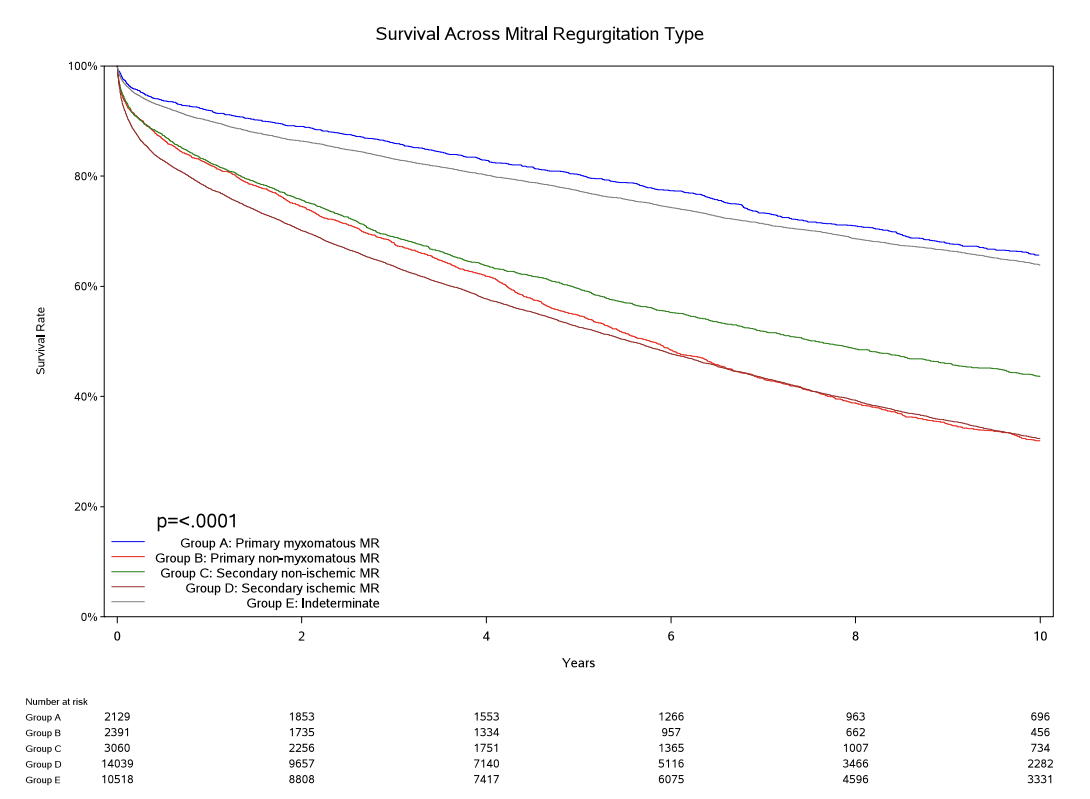
\includegraphics[width=1.0\linewidth]{images/teer/fig MR type severity prognosis.png}
    \caption{Unadjusted Survival Curves for Different Etiologies of ≥ Mild MR. Unadjusted survival of patients with ≥mild MR stratified by etiology. Abbreviations: MR, mitral regurgitation.\cite{Samad2013}}
    \label{images/teer/fig MR type severity prognosis}
\end{figure}

\subsection{What is tethering?}
\textbf{Tethering是什麼意思?} 

二尖瓣牽拉（Mitral Valve Tethering）是指二尖瓣葉片因周圍結構的牽引而導致運動受限的現象。這通常發生在左心室擴大或重構時，乳頭肌的位置改變，導致腱索拉緊，限制葉片的正常閉合功能。結果，二尖瓣無法完全閉合，導致血液在心臟收縮期間從左心室逆流回左心房，形成二尖瓣逆流（Mitral Regurgitation）。

此現象在繼發性二尖瓣逆流（Secondary Mitral Regurgitation）中尤為常見，特別是由於心肌梗塞或擴張型心肌病變引起的左心室重構。牽拉程度可通過心臟超音波等影像學技術評估，這對於診斷和治療策略的制定具有重要意義。\cite{Grayburn2021}


\subsection{Echocardiographic evaluation- repair feasibility}
在術前評估上與許多要測量的項目，這些都是在MPR (multi-plane reconstruction)影像下進行會較方便 (Figure ~\ref{images/teer/fig TEER TEE leaflet length})。
Measurement for leaflet grasping (mandatory in Mainz):
\begin{itemize}
    \item Mitral annular diameter: AP and intercommissural planes: > 38-40 mm for XTW or XT
    \item Mitral valve area: > 4 cm2
    \item Grasping zone leaflet mobile length
\end{itemize}

\begin{figure}
    \centering
    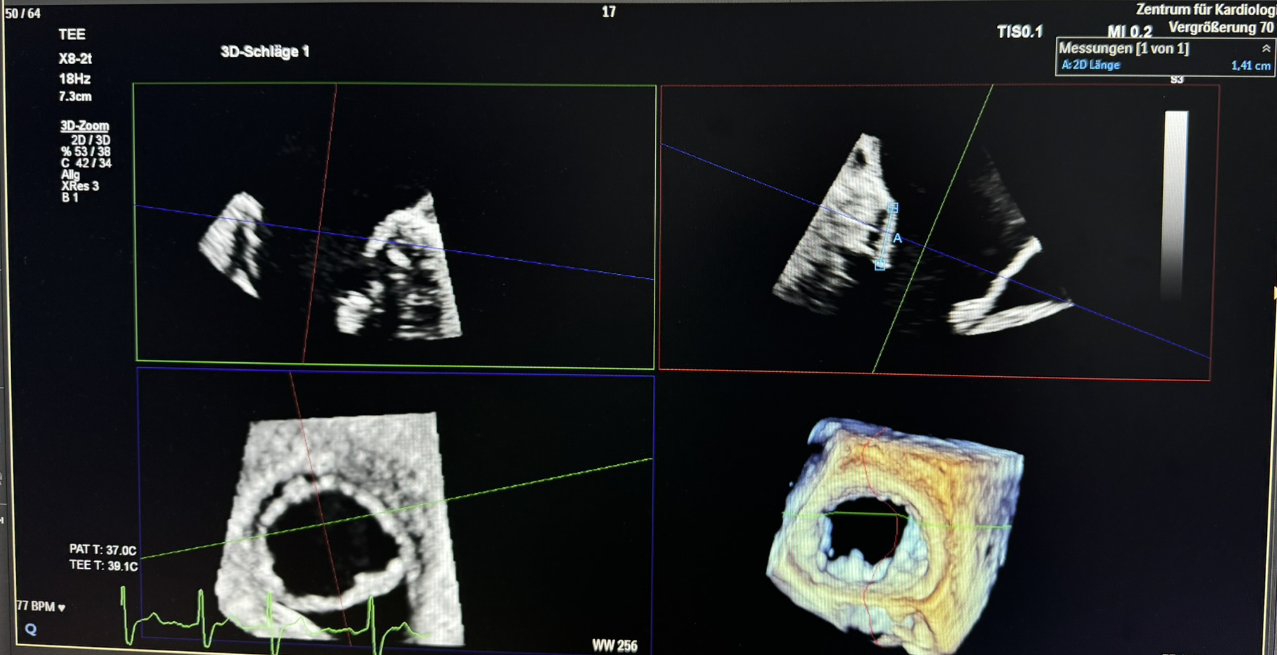
\includegraphics[width=0.9\linewidth]{images/teer/fig TEER TEE leaflet length.png}
    \caption{MPR, multiplanar reconstruction, 可以在這裡確認各項測量指標彼此相對的位置與關係。}
    \label{images/teer/fig TEER TEE leaflet length}
\end{figure}

\subsection{The Carpentier classification}

\begin{figure}[h]
  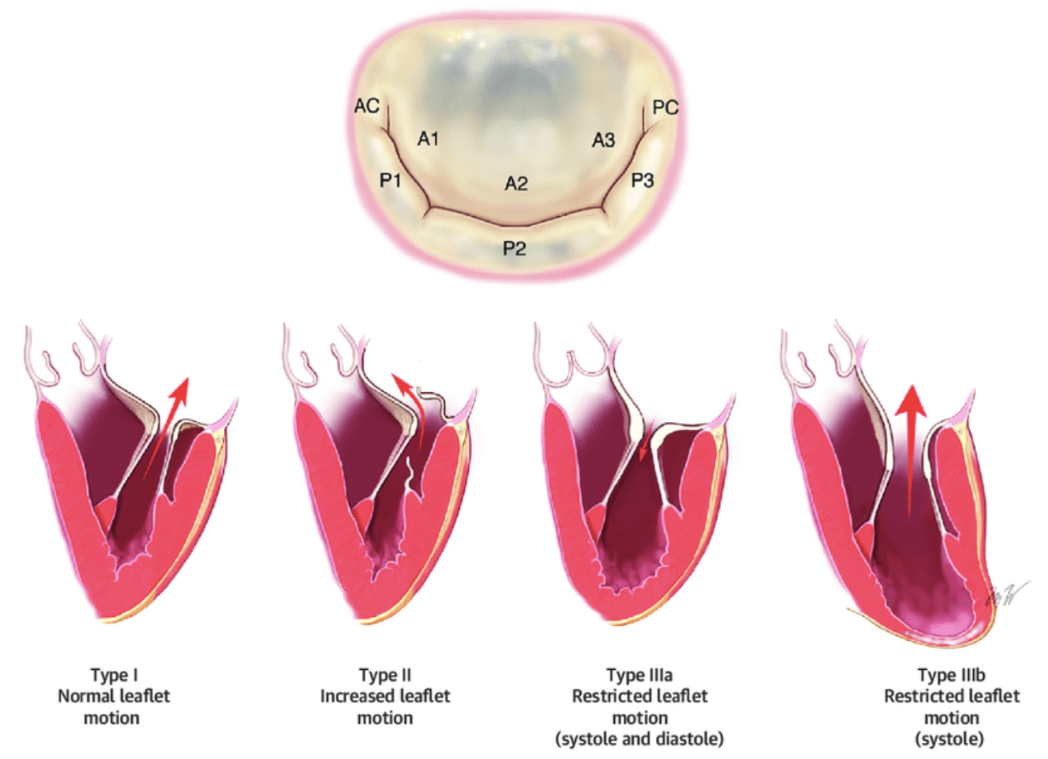
\includegraphics[width=\linewidth]{images/teer/fig Carpentier classification.png}
  \caption{Carpentier classification. Carpentier classification 是針對二尖瓣閉鎖不全（Mitral Regurgitation, MR）的分類系統，根據二尖瓣的解剖學和功能異常，分為三種主要的類型，用以協助描述疾病機制並指導手術治療策略。\cite{Carpentier1983, Grayburn2021}}
  \label{images/teer/fig Carpentier classification}
\end{figure}

\begin{longtable}{p{3cm} p{7cm}}
\caption{Carpentier classification of MR/TR}\\
\hline
\textbf{Class} & \textbf{Description} \\
\hline
\endfirsthead
\multicolumn{2}{l}{\textit{接續上一頁}} \\
\hline
\textbf{項目} & \textbf{內容} \\
\hline
\endhead
\hline \multicolumn{2}{r}{\textit{接續下一頁}} \\
\endfoot
\endlastfoot

\textbf{類型 I：正常瓣膜運動} & 
這類 MR 的主要病因通常是二尖瓣環的擴張，導致瓣膜的對合（coaptation）不良。
病例常見於功能性 MR，例如與左心房擴大相關的情況。
\\ \hline

\textbf{類型 II：瓣膜運動過度} & 
此類型與瓣膜的過度移動有關，通常為脫垂prolapse或flail leaflet. 
瓣膜脫垂是原發性 MR（Primary Mitral Regurgitation, PMR）的主要病因。
\\ \hline

\textbf{類型 III：瓣膜運動受限} &
\begin{itemize}
    \item 類型 IIIa：收縮期與舒張期皆受限。病因多為瓣膜病變，如風濕性心臟病、放射線後遺症或其他炎性狀況，這些情況通常導致瓣膜變形與纖維化。
    \item 類型 IIIb：僅於收縮期受限。與左心室重構（ventricular remodeling）及擴張有關，導致瓣膜小葉在收縮期間運動受限。此類型常見於缺血性或非缺血性功能性 MR，亦可能與乳頭肌功能障礙或瓣膜運動不同。
    \item 其中，又可以將restricted leaflet motion區分為symmetrical restriction (如DCMP-related ventricular dilatation)與asymmetrical restriction (如ischemic cardiomyopathy造成posterior leaflet tethering). 
\end{itemize}
\\ \hline


\end{longtable}


\subsection{Echocardiographic evaluation- severity}
二尖瓣逆流（Mitral Regurgitation, MR）的分級基於多參數的整合評估方法，包括定性（Qualitative）、半定量（Semi-Quantitative）和定量（Quantitative）指標（見表1）。定義重度 MR 的主要定量超音波參數包括：

\begin{itemize}
    \item 瓣口頸部寬度（Vena Contracta width）：$\geq$ 7 mm
    \item 逆流分數（Regurgitant Fraction）：$\geq$ 50\%
    \item 有效逆流口面積（Effective Regurgitant Orifice Area, EROA）：$\geq$ 40 mm²
    \item 逆流量（Regurgitant Volume, RVol）：$\geq$ 60 ml
\end{itemize}

上面提到的數字，若是病人有DCMP, 有較低的心輸出量，就要注意EROA, RVol這兩個數字條件就不能訂得太高。基於 PISA（Proximal Isovelocity Surface Area）的有效逆流口面積（Effective Regurgitant Orifice Area, EROA）和逆流量（Regurgitant Volume, RVol）的評估，對於繼發性二尖瓣反流（Secondary Mitral Regurgitation, SMR）患者應謹慎使用。建議參考VCW and regurgitant fraction進行整合評估。\cite{Hausleiter2023}


\begin{longtable}{p{3cm} p{7cm}}
\caption{Mainz Heart Valve Center的常看指標}
\hline
\textbf{指標} & \textbf{說明} \\ \hline
\endfirsthead
\hline
\textbf{指標} & \textbf{說明} \\ \hline
\endhead
\hline
\endfoot
Vena contracta width & 大於或等於 7 mm，為診斷重度二尖瓣逆流的可靠定量指標。 \\ \hline
E-velocity & 大於 1.5 m/sec，提示顯著的血流速度增強，與severe MR 相關。 \\ \hline
VTI of MR & 大於 1.4，表示二尖瓣逆流的時間-速度積分增高。 \\ \hline
Pulmonary vein flow reversal & 出現肺靜脈血流逆向，提示MR嚴重影響左心房血流動力學。 \\ \hline
\end{longtable}

\begin{marginfigure}
    \centering
    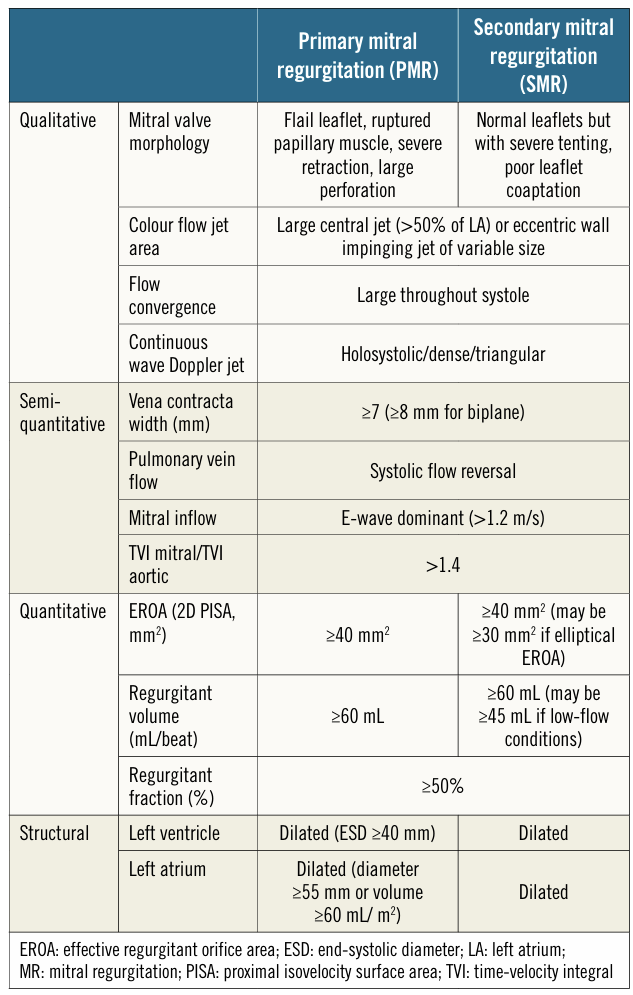
\includegraphics[width=1.0\linewidth]{images/teer/fig MR severity table from EI.png}
    \caption{Quantification of severe MR.\cite{Hausleiter2023}}
    \label{images/teer/fig MR severity table from EI}
\end{marginfigure}

\subsection{When should we NOT proceed with M-TEER?}
什麼時候不該考慮 M-TEER? 在Mainz嚴格遵守下面條件，因為一旦治療後導致 severe mitral stenosis, 病患可能會在2-6小時內直接因為急性肺水腫導致臨床狀況惡化。
\begin{itemize}
    \item Annular diameter (anterior-posterior) < 30 mm.
    \item Severe valve calcification.
    \item Resting mitral inflow pressure gradient $\geq$ 5 mmHg. 
\end{itemize}

\section{Special note on patients with very low LVEF}
病人若是LVEF已經很差了，這個時候ERO and regurgitant volume (RV)都可能低估瓣膜逆流的嚴重度。因為LV contractility已經很差，所以可以導致ERO and RV測量不準。在2024-11-12的case 19 (Figure ~\ref{images/teer/fig TEER case 19}) 就看到明明MR color mapping下jet很大，佔了LA 40\% area, 但是測量的ERO只有0.1 cm$^2$, RV只有12 ml. 怎麼看都不對。但是該例的 vena contracta width則有13 mm, 而且有明顯的pulmonary vein flow reversal (還是會據此判斷為severe MR).

\begin{figure}
    \centering
    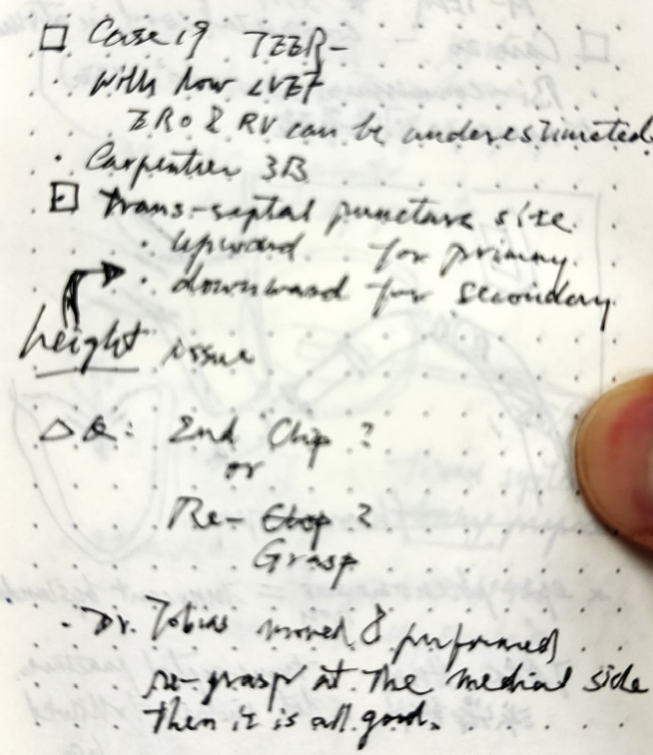
\includegraphics[width=0.75\linewidth]{images/teer/fig TEER case 19.png}
    \caption{Case 19, 2024-11-12}
    \label{images/teer/fig TEER case 19}
\end{figure}

\section{MV anatomy}
Indentation lines: 大部份都在 posterior leaflet 被看到。而indentation對於M-TEER會產生直接影響，讓leaflet tension分佈不均，且可讓M-TEER MR改善不如預期。

Findings suggestive of only mild MR:
\begin{itemize}
    \item prominent A
\end{itemize}

%\section{Identification of pulmonary veins}

%\section{TR evaluation}

\newpage
\section{Interventional TEE (iTEE)}
Mainz protocol: aorta be positioned at 6 o'clock (En Face view). 

\subsection{Interventional TEE and setting in the hybrid OR}
在hybrid OR裡面，專屬的C-arm為single arm, 位置在病患的左側，將頭側保留給interventional TEE operator, 以及麻醉科醫師。採用single arm, 所以頭側的空間可以很大。(Figure ~\ref{images/teer/fig TEER setting}) 同時可以直接輸入麻機生理監視器的心電圖訊號到心臟超音波檢查儀中，以減少重覆接線。(Figure ~\ref{images/teer/fig TEER ECG connection, fig TEER echo operator})

\begin{figure}
    \centering
    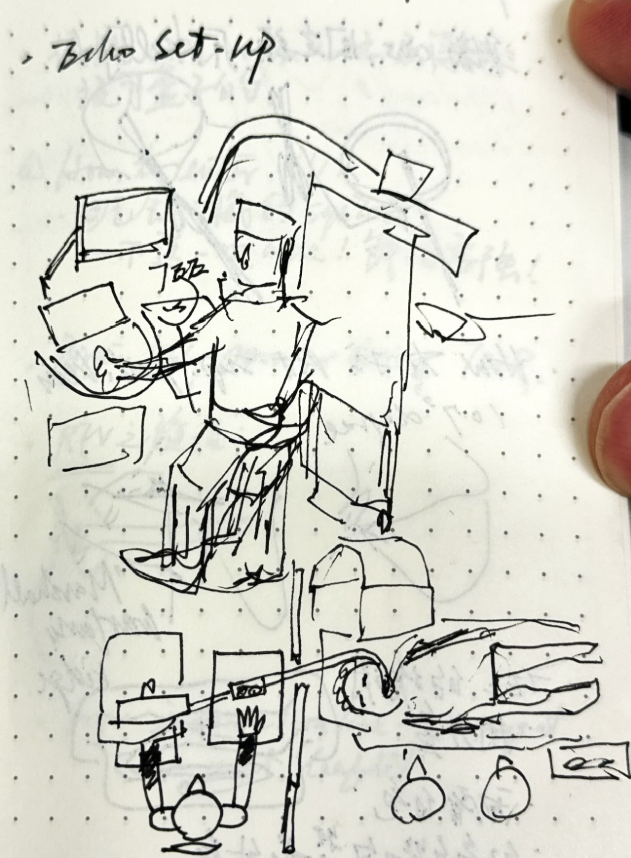
\includegraphics[width=1\linewidth]{images/teer/fig TEER echo operator.png}
    \caption{執行TEE會有不必要的輻射暴露，所以TEE operator務必要以鉛玻璃屏風保護自己。}
    \label{images/teer/fig TEER echo operator}
\end{figure}

\begin{figure}
    \centering
    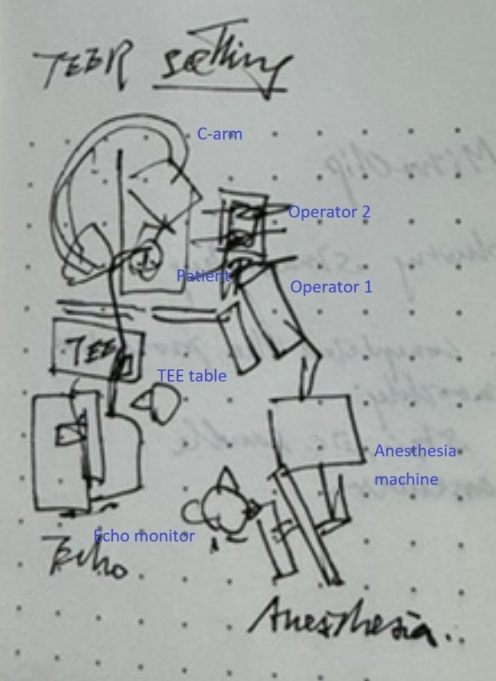
\includegraphics[width=0.8\linewidth]{images/teer/fig TEER setting.jpg}
    \caption{Operator 1 以及 operator 2站在病患右側，interventional TEE的畫面經由Philips系統投射在主螢幕上。Hybrid OR只有single arm, 並且將病患的頭側保留給麻醉機以及interventional TEE operator. 值得注意的是: 頭側用兩片很大的鉛玻璃進行輻射防護。}
    \label{images/teer/fig TEER setting}
\end{figure}

\begin{figure}
    \centering
    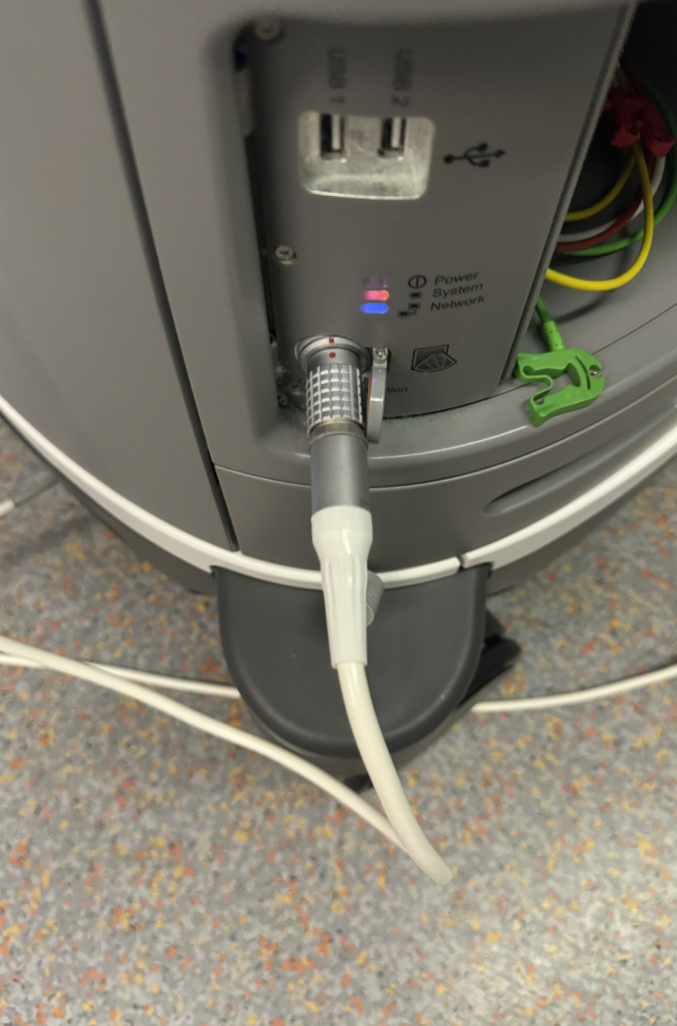
\includegraphics[width=0.75\linewidth]{images/teer/fig TEER ECG connection.png}
    \caption{在TEER執行時，為了減少重覆接線，可以直接將echo machine接受麻醉機生理監視器的訊號線。}
    \label{images/teer/fig TEER ECG connection}
\end{figure}

\begin{marginfigure}
%\vskip -1.2in
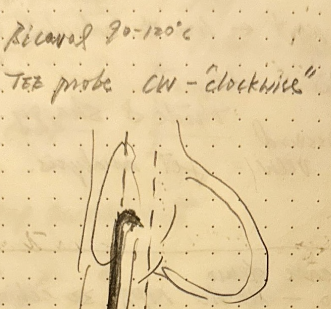
\includegraphics{images/teer/fig TEER TEE bicaval.png}
\caption{Bi-caval view是用來一開始穿刺完靜脈，要準備進行trans-septal puncture重要的view. }
\label{images/teer/fig TEER TEE bicaval}
\end{marginfigure}


介入經食道超音波（iTEE）在心血管介入治療中的地位愈來愈重要，其主要功能是為複雜的心臟手術與經皮介入治療提供即時的高解析影像指引。其重要性體現在以下幾個方面：




\begin{itemize}
    \item \textbf{即時引導與監測}
    \begin{itemize}
        \item 為經皮介入手術（如二尖瓣經導管緣對緣修復 [M-TEER]、經導管主動脈瓣置換術 [TAVI]）提供關鍵的影像引導，確保手術精確性。
        \item 能即時監測手術過程中的瓣膜功能、裝置位置及併發症情況，如瓣膜漏失或血栓形成。
    \end{itemize}

    \item \textbf{解剖與功能性評估}
    \begin{itemize}
        \item 提供二尖瓣、三尖瓣等心臟瓣膜的詳細解剖結構信息，特別適用於瓣膜病變或複雜結構異常患者。
        \item 協助量化心臟功能參數，例如有效反流口面積（Effective Regurgitant Orifice Area, EROA）及反流體積（Regurgitant Volume, RVol）。
    \end{itemize}

    \item \textbf{高解析影像與多平面能力}
    \begin{itemize}
        \item iTEE 使用 3D 成像技術，能提供傳統經胸超音波（TTE）難以達到的視角，如心臟後方結構。
        \item 多平面功能使得操作者能在不同角度下快速調整影像，精確定位介入設備與治療目標。
    \end{itemize}
\end{itemize}

iTEE是怎麼發展的?

\begin{itemize}
    \item \textbf{早期發展}
    \begin{itemize}
        \item 經食道超音波（TEE）的應用始於 20 世紀 70 年代，當時主要用於術中心臟手術監測。
        \item 隨著超音波技術的進步，特別是 3D 成像與即時影像處理的發展，iTEE 的潛力逐漸被醫學界認識。
    \end{itemize}

    \item \textbf{進一步應用於介入治療}
    \begin{itemize}
        \item 2000 年代初，iTEE 開始被引入心血管介入手術，如 TAVI 和 M-TEER，因其能解決傳統影像工具（如透視）對軟組織顯像不足的問題。
        \item 使用 3D iTEE 提升了瓣膜修復手術的成功率，並減少了併發症風險。
    \end{itemize}

    \item \textbf{現代技術與整合}
    \begin{itemize}
        \item 現代 iTEE 與其他成像技術（如 CT 或 MRI）結合，形成多模態成像，提供術前計劃與術中指引。
        \item 融合導航技術（fusion imaging）進一步強化了 iTEE 在導引裝置操作及定位上的作用。
    \end{itemize}
\end{itemize}




\begin{marginfigure}[h]
    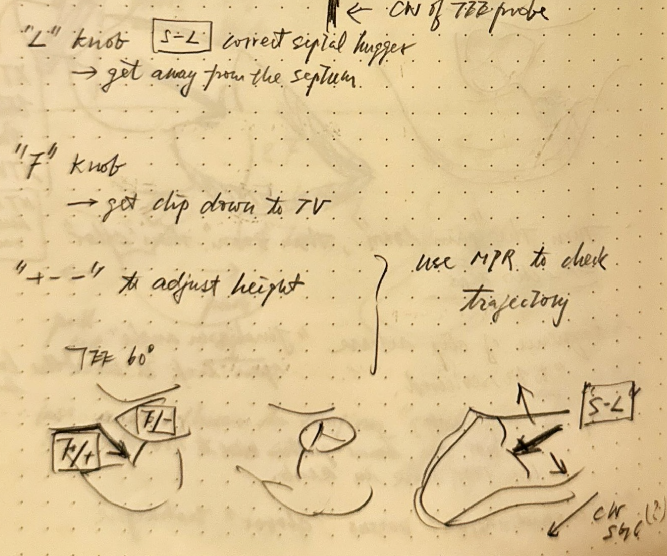
\includegraphics{images/teer/fig TEER TV knobology 1.png}
    \caption{T-TEER的操作重點，在圖中可以看到S/L knob, 以及 F/E knob的功能。}
    \label{images/teer/fig TEER TV knobology 1}
\end{marginfigure}

\begin{marginfigure}
\vskip -1.2in
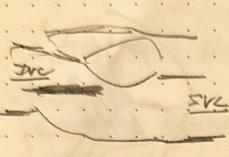
\includegraphics{images/teer/fig TEER SVC IVC.png}
\caption{Bi-caval view是用來一開始穿刺完靜脈，要準備進行trans-septal puncture重要的view. }
\label{images/teer/fig TEER SVC IVC}
\end{marginfigure}

\subsection{Jet analysis}
Jet analysis, 指的是針對color mapping下的jet, 用下面流程，找到相對應的leaflet pathology，再進行治療的過程。

\begin{itemize}
    \item 2D echo to identify leaflet motion, coaptation, any sign of chordae rupture.
    \item 2D color mapping to have an initial impression of the jet locaiton, width, and direction.
    \item 2D echo with X-plane, without color, using X-plane "sweeping" method to identify leaflet pathology.
    \item 2D color mapping with X-plane, to further confirm the pathology relation to jet.
    \item 3D echo, with MPR, to evaluation if there is any jet missed from the previous evaluation sequence.
\end{itemize}

\begin{figure}
    \centering
    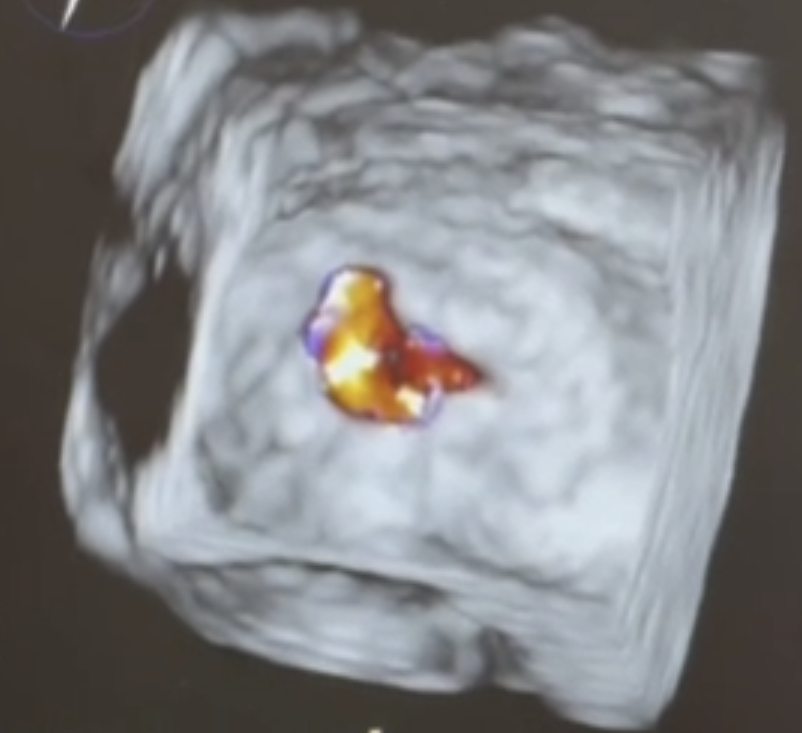
\includegraphics[width=1\linewidth]{images/teer/fig TEER jet analysis 3D.png}
    \caption{Jet analysis是整個TEER治療當中相當重要的環節，在Mainz看到的是依序使用 X-plane, 3D, 最後是MPR進行jet analysis. 關鍵並不是jet的位置與方向，而是循著jet找到相對應的leaflet pathology並針對該位置進行治療。}
    \label{images/teer/fig TEER jet analysis 3D}
\end{figure}


\section{Treatment algorithm}
患者的治療建議：針對以下患者的治療策略：(A) 有症狀的重度原發性二尖瓣反流（Primary Mitral Regurgitation, MR）或 (B) 有症狀的重度繼發性二尖瓣反流（Secondary MR）。請參考 Figure ~\ref{images/teer/fig TEER treatment algorithm}. 


\begin{itemize}
    \item COAPT：功能性二尖瓣反流患者使用 MitraClip 經皮治療的心血管結果評估（Cardiovascular Outcomes Assessment of the MitraClip Percutaneous Therapy for Heart Failure Patients With Functional Mitral Regurgitation）。
    \item GDMT：指導性醫療治療（Guideline-Directed Medical Therapy）。
    \item HTx：心臟移植（Heart Transplantation）。
    \item LVAD：左心室輔助裝置（Left Ventricular Assist Device）。
    \item M-TEER：二尖瓣經導管緣對緣修復（Mitral Valve Transcatheter Edge-to-Edge Repair）。
    \item SMVR：二尖瓣外科修復或置換（Surgical Mitral Valve Repair or Replacement）。
\end{itemize}

\begin{figure}
    \centering
    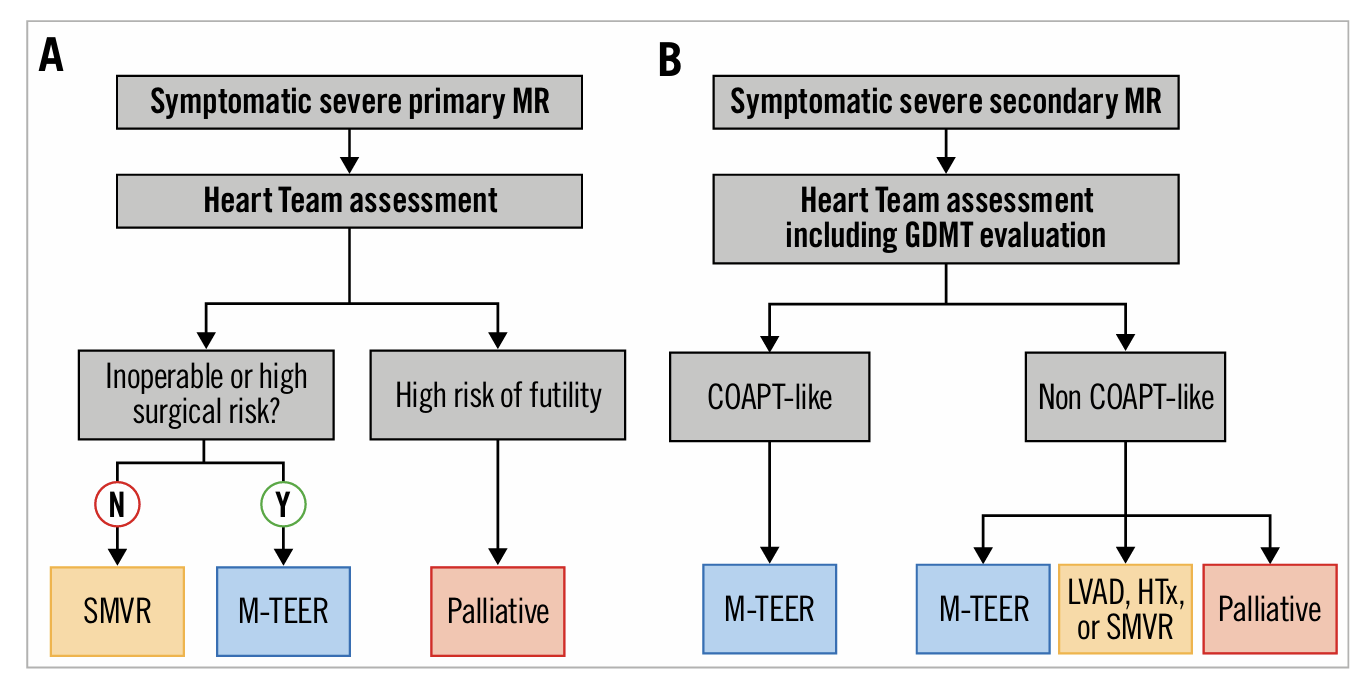
\includegraphics[width=1\linewidth]{images/teer/fig TEER treatment algorithm.png}
    \caption{Patient stratification and simplified guideline recommendation. Therapeutic strategies for patients with (A) symptomatic severe primary mitral regurgitation (MR) or (B) symptomatic severe secondary MR.\cite{Hausleiter2023}}
    \label{fig treatment}
\end{figure}
\newpage

\section{TEER repair systems}

\begin{figure}
    \centering
    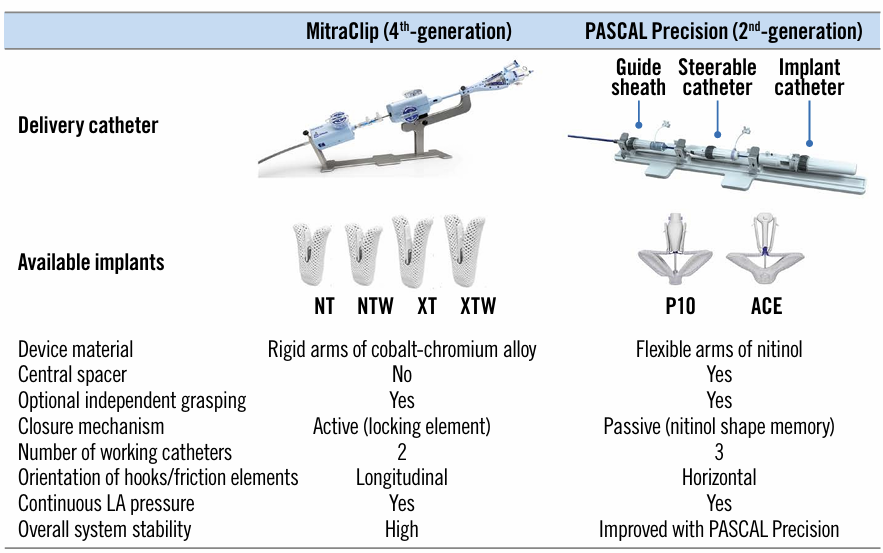
\includegraphics[width=1\linewidth]{images/teer/fig TEER systems.png}
    \caption{目前在歐洲獲准用於二尖瓣（Mitral Valve, MV）微創治療的兩種二尖瓣經導管緣對緣修復（M-TEER）設備為 MitraClip 系統（由 Abbott 製造）和 PASCAL 系統（由 Edwards Lifesciences 製造）。Table ~\ref{table TEER systems}是這兩種平台的主要差異說明。}
    \label{images/teer/fig TEER systems}
\end{figure}

\begin{longtable}{ p{2cm} p{4cm} p{4cm}}
\caption{MitraClip/TriClip與PASCAL的比較}
\label{table TEER systems}
\hline
\textbf{特性} & \textbf{MitraClip/TriClip 系統} & \textbf{PASCAL 系統} \\ \hline
\endfirsthead
\hline
\textbf{特性} & \textbf{MitraClip/TriClip 系統} & \textbf{PASCAL 系統} \\ \hline
\endhead
\hline
\endfoot
製造商 & Abbott & Edwards Lifesciences \\ \hline
材質 & 剛性臂由鈷鉻合金製成 & 柔性臂由鎳鈦合金製成 \\ \hline
中央間隔 (Spacer) & 無中央間隔 (Spacer) & 配備中央間隔，有機會減少被瓣葉鍵索困住的機會 \\ \hline
抓握方式 & 支援前後葉的獨立抓握 & 支援前後葉的獨立抓握 \\ \hline
閉合機制 & 主動閉合（鎖定元件） & 被動閉合（鎳鈦形狀記憶） \\ \hline
夾子尺寸 & 提供多種尺寸選項（例如 NT, XT） & 提供標準版與 Ace 小型版 \\ \hline
導引穩定性 & 高穩定性 & 改良版 PASCAL Precision 系統提升穩定性 \\ \hline
\end{longtable}

\subsection{MitraClip}
如何選夾子的大小? 這個在MitraClip因為有很多選擇，其實學問滿大的!

\marginnote{
If annular diameter > 40 mm, always consider MitraClip XT or XTW first. 
If annular diameter < 35 mm, the only options are MitraClip NT or NTW. 
}

\subsection{PASCAL}
可以用於進行 M-TEER and T-TEER. \cite{Fam2018} 

First reported the use to PASCAL to treat severe TR. Reported PASCAL use as compassionate therapy for patients with severe TR.\cite{Fam2019} 

\section{TEER procedure steps}

\subsection{Preparation of MitraClip/TriClip}

\begin{figure}[ht]
    \centering
    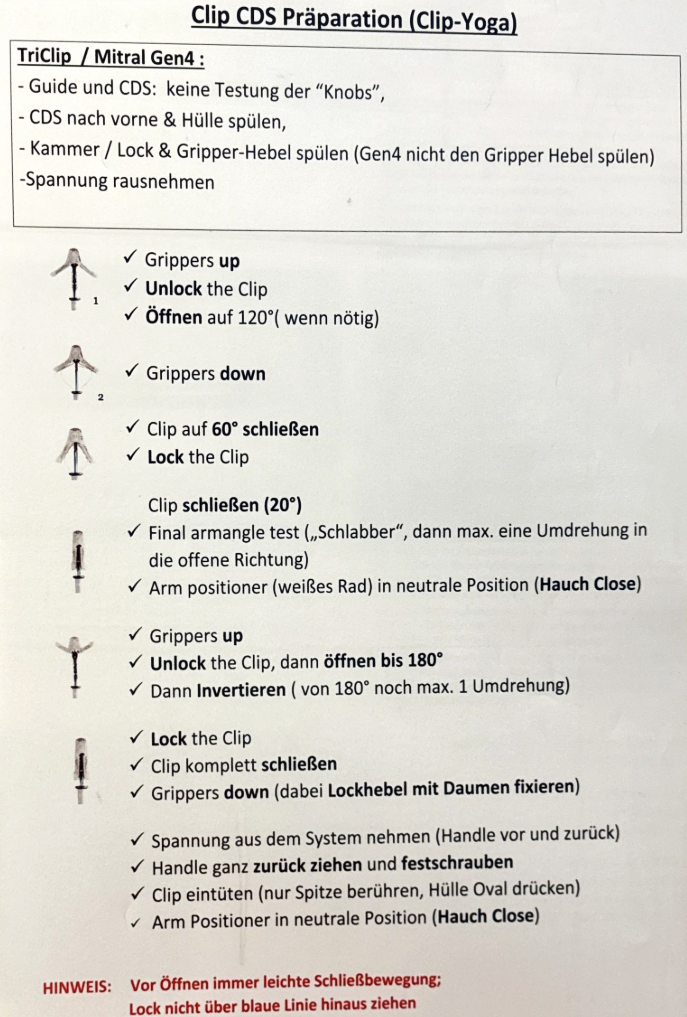
\includegraphics[width=0.7\linewidth]{images/teer/fig_TEER clip preparation.png}
    \caption{這是在Mainz hybrid OR牆上的clip準備說明。}
    \label{TEER clip preparation}
\end{figure}

\subsection{Steerable guiding catheter (SGC) placement}
heparin: 在SGC擺好後才注射

\subsection{Use of fluoroscopy}
Fluoroscopy透視攝影並不會被interventional TEE取代，在進行TEER時，都會需要打到RAO，並加上cranial or caudal, 將clip在fluoroscopy好好打開關起來並檢視，是否在進入ventricle之後，沒有改辦clocking的角度。\cite{Zoghbi2017}

在fluoroscopy定位好後，在將clip進入到ventricle後，都可以再用fluoroscopy確認是否clocking有改變。


\subsection{Transseptal puncture}

\subsection{Before the era of interventional TEE}
% Nunes2016 figure is great!

\begin{figure}
    \centering
    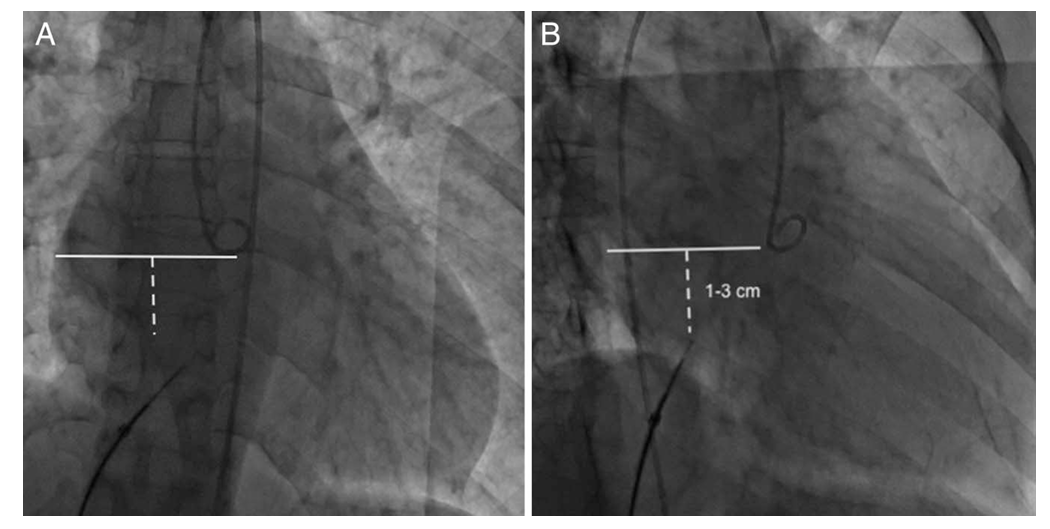
\includegraphics[width=1.0\linewidth]{images/teer/fig fluoroguided transseptal.png}
    \caption{The flouroscopy-guided transseptal puncture landmarks. (A) In the anteroposterior  projection, the puncture site should be halfway from the distance of the  catheter and the right border of the left  atrium and one vertebral body height lower to the aortic valve plane (seen by inserting a pig tail catheter in the non-coronary aortic sinus). (B) In the 40° right anterior oblique projection, confirm if the needle is positioned neither close to the aortic root (too anterior) nor close to the free wall of the right atrium (too posterior). The  puncture site should be 1–3 cm below the midpoint of a line connecting the posterior wall of the aorta to the back wall of the right atrium.}
    \label{images/teer/fig fluoroguided transseptal}
\end{figure}


\subsection{In the era of interventional TEE}

針頭 (Brockenbrough needle) 和導管鞘 (Mullin sheath)需用手指固定，以防止針頭意外前進，並根據不同的操作將 Brockenbrough 針的箭頭位置調整至 5 點鐘或 6 點鐘方向（如圖 4 所示）。若需針對更靠後的位置穿刺，應將箭頭保持在 6 點鐘方向。將針頭和導管鞘向尾側拉回，直至它們在上腔靜脈（SVC）下部被可被TEE看到。穿刺時，應在經TEE下進行。

The needle and the sheath are held in the fingers to prevent inadvertent advancement of the needle, and the position of the Brockenbrough needle arrow is at 5 or 6 o’clock, according to different procedures (Figure 4). To target a more posterior puncture location, the arrow should be kept at the 6 o’clock position. The needle and the sheath are pulled back caudally until they are visualized in the inferior portion of the SVC. Tenting should be monitored by echocardiography (bicaval view) in the lower part of the SVC before the needle falls into the fossa. Usually, as the needle tents the superior rim of the fossa, supraventricular extrasystolic beats are generated. During this phase, the TEE operator should avoid moving the image from the membranous portion of the septum, and the interventionalist should try to move in the direction of the image.

\begin{figure}
    \centering
    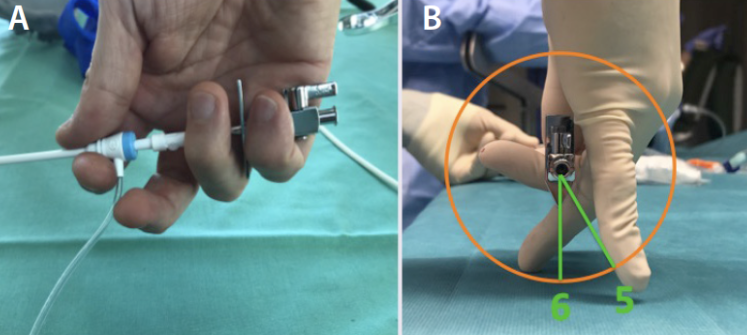
\includegraphics[width=1\linewidth]{images/teer/fig TEER SP BK direction.png}
    \caption{Correct handling (A) and orientation (B) of the Mullins sheath and Brockenbrough needle during the pullback maneuvers. Figure from \href{https://citoday.com/articles/2019-may-june/transseptal-puncture-a-step-by-step-procedural-guide}{https://citoday.com/articles/2019-may-june/transseptal-puncture-a-step-by-step-procedural-guide}}
    \label{images/teer/fig TEER SP BK direction}
\end{figure}

在這一步驟中，透視（正位投影，AP projection）具有兩個作用：（1）監測針尖的位置（AP 旋轉）直至其落入卵圓窩內；（2）避免過度向下拉至下腔靜脈。

\begin{figure}
    \centering
    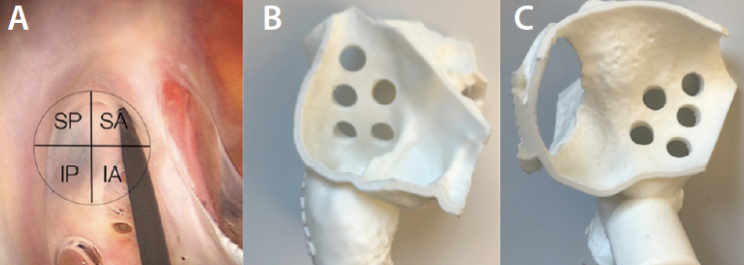
\includegraphics[width=1.0\linewidth]{images/teer/fig TEER TS anatomy.png}
    \caption{Fossa ovalis anatomy from the RA view and its schematic division into four parts (A). Three-dimensional models showing the IS from the right side (B) and the left side (C). IA, inferior-anterior; IP, inferior-posterior; SA, superior-anterior; SP, superior-posterior. Figure from \href{https://citoday.com/articles/2019-may-june/transseptal-puncture-a-step-by-step-procedural-guide}{https://citoday.com/articles/2019-may-june/transseptal-puncture-a-step-by-step-procedural-guide}}
    \label{images/teer/fig TEER TS anatomy}
\end{figure}

接著，在經食道超聲心動圖（TEE，雙腔視角）的監測下，將針頭和導管鞘向後拉，直至進入卵圓窩並形成“頂撐”（tenting）（圖 5A）。此時，TEE 切換至短軸（SAX）基底視角，檢查“頂撐”的位置；對於大多數接受二尖瓣介入治療的患者，“頂撐”應位於後側（圖 5B）。

一旦transseptal系統進入卵圓窩內，若需要調整位置，operator必須同時進行兩個方向的移動，以防止針頭產生支點旋轉。僅進行順時針旋轉會導致導管鞘旋轉，但接觸點不會改變。若需向後移動，operator需要結合旋轉動作與輕微拉回導管，以便調整針尖的位置——如果“頂撐”位置過於靠前，可在透視指引下施加針頭的順時針扭力，同時進行輕微的回拉動作，使其移動至後方；若“頂撐”位置過於靠後，則需施加逆時針旋轉，並同步進行回拉動作。

在進行 MitraClip（Abbott Vascular）操作時，TEE應切換至4-chamber view (四腔心視角)，並測量穿刺高度（即“頂撐”位置與二尖瓣環之間的距離, tenting point to mitral annulus distance）（圖 5C）。對於退化性二尖瓣逆流患者 (Carpentier classification II)，理想的高度應大於 4 公分；而在功能性二尖瓣逆流患者中 (Carpentier classification III)，3.5 公分的距離是可以接受的。由於膜性隔具有彈性，在操作裝置時穿刺高度可能會降低，因此，若存在鬆軟的心房中隔，建議選擇更高的位置進行穿刺。

\begin{figure}
    \centering
    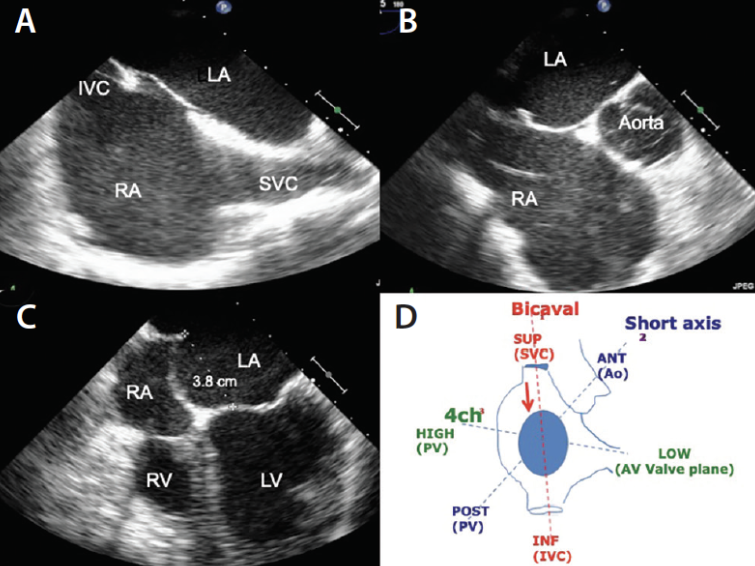
\includegraphics[width=1\linewidth]{images/teer/fig TEER TS TEE.png}
    \caption{TEE bicaval view (A), SAX at the base view (B), and four-chamber view (C) during the pullback phase of TP. Schematic view of the three main TEE projections used during TP in relation to the anatomic structures they show (D). 4ch, four chamber; ANT, anterior; Ao, aorta; AV valve, atrioventricular valve; INF, inferior; IVC, inferior vena cava; LV, left ventricle; PV, pulmonary vein; RV, right ventricle; SUP, superior. Figure from \href{https://citoday.com/articles/2019-may-june/transseptal-puncture-a-step-by-step-procedural-guide}{https://citoday.com/articles/2019-may-june/transseptal-puncture-a-step-by-step-procedural-guide}}
    \label{images/teer/fig TEER TS TEE}
\end{figure}


穿刺的理想位置取決於所使用的特定設備和患者的特徵。MitraClip 手術通常選擇後方的穿刺位置，位於上後和下後區域；Cardioband（Edwards Lifesciences）手術則多選擇更靠前的穿刺位置（上前和下前區域）；而LAAO (左心耳封堵術)通常通過下方的穿刺位置進行（通常位於下後區域）。主要的 TEE 投影及相關的可見解剖結構如圖 5D 所示。

TEE（經食道超聲心動圖）應切換至短軸（SAX）視角，透視（Fluoroscopy）應保持在正位投影（AP projection）。在這一步驟中，針頭需在保持經隔導管鞘固定不動的情況下向前推進。在此階段，操作應採用緩慢的動作，以防系統滑動至上腔靜脈（SVC）過於靠前（朝向主動脈）或過於靠後（朝向 Waterston 溝）。

為了降低這些風險，作為傳統技術的替代方法，穿刺過程可輔以使用電灼手術系統或射頻（RF）經隔穿刺系統（NRG RF Transseptal Kit，Baylis Medical Company, Inc.），以提升穿刺的安全性與精確性。

通常，在穿刺卵圓窩後，“頂撐”（tenting）會在 TEE 中消失。為了進一步提高安全性，在推進經隔導管鞘之前，應確認左心房壓力。如果未見壓力曲線，或者發現主動脈壓力，不應推進導管鞘。完成穿刺後，應追加肝素劑量以達到完全抗凝（100 U/kg），目標活化凝血時間（ACT）應維持在 250 至 300 秒，適用於大多數手術操作。

\begin{figure}
    \centering
    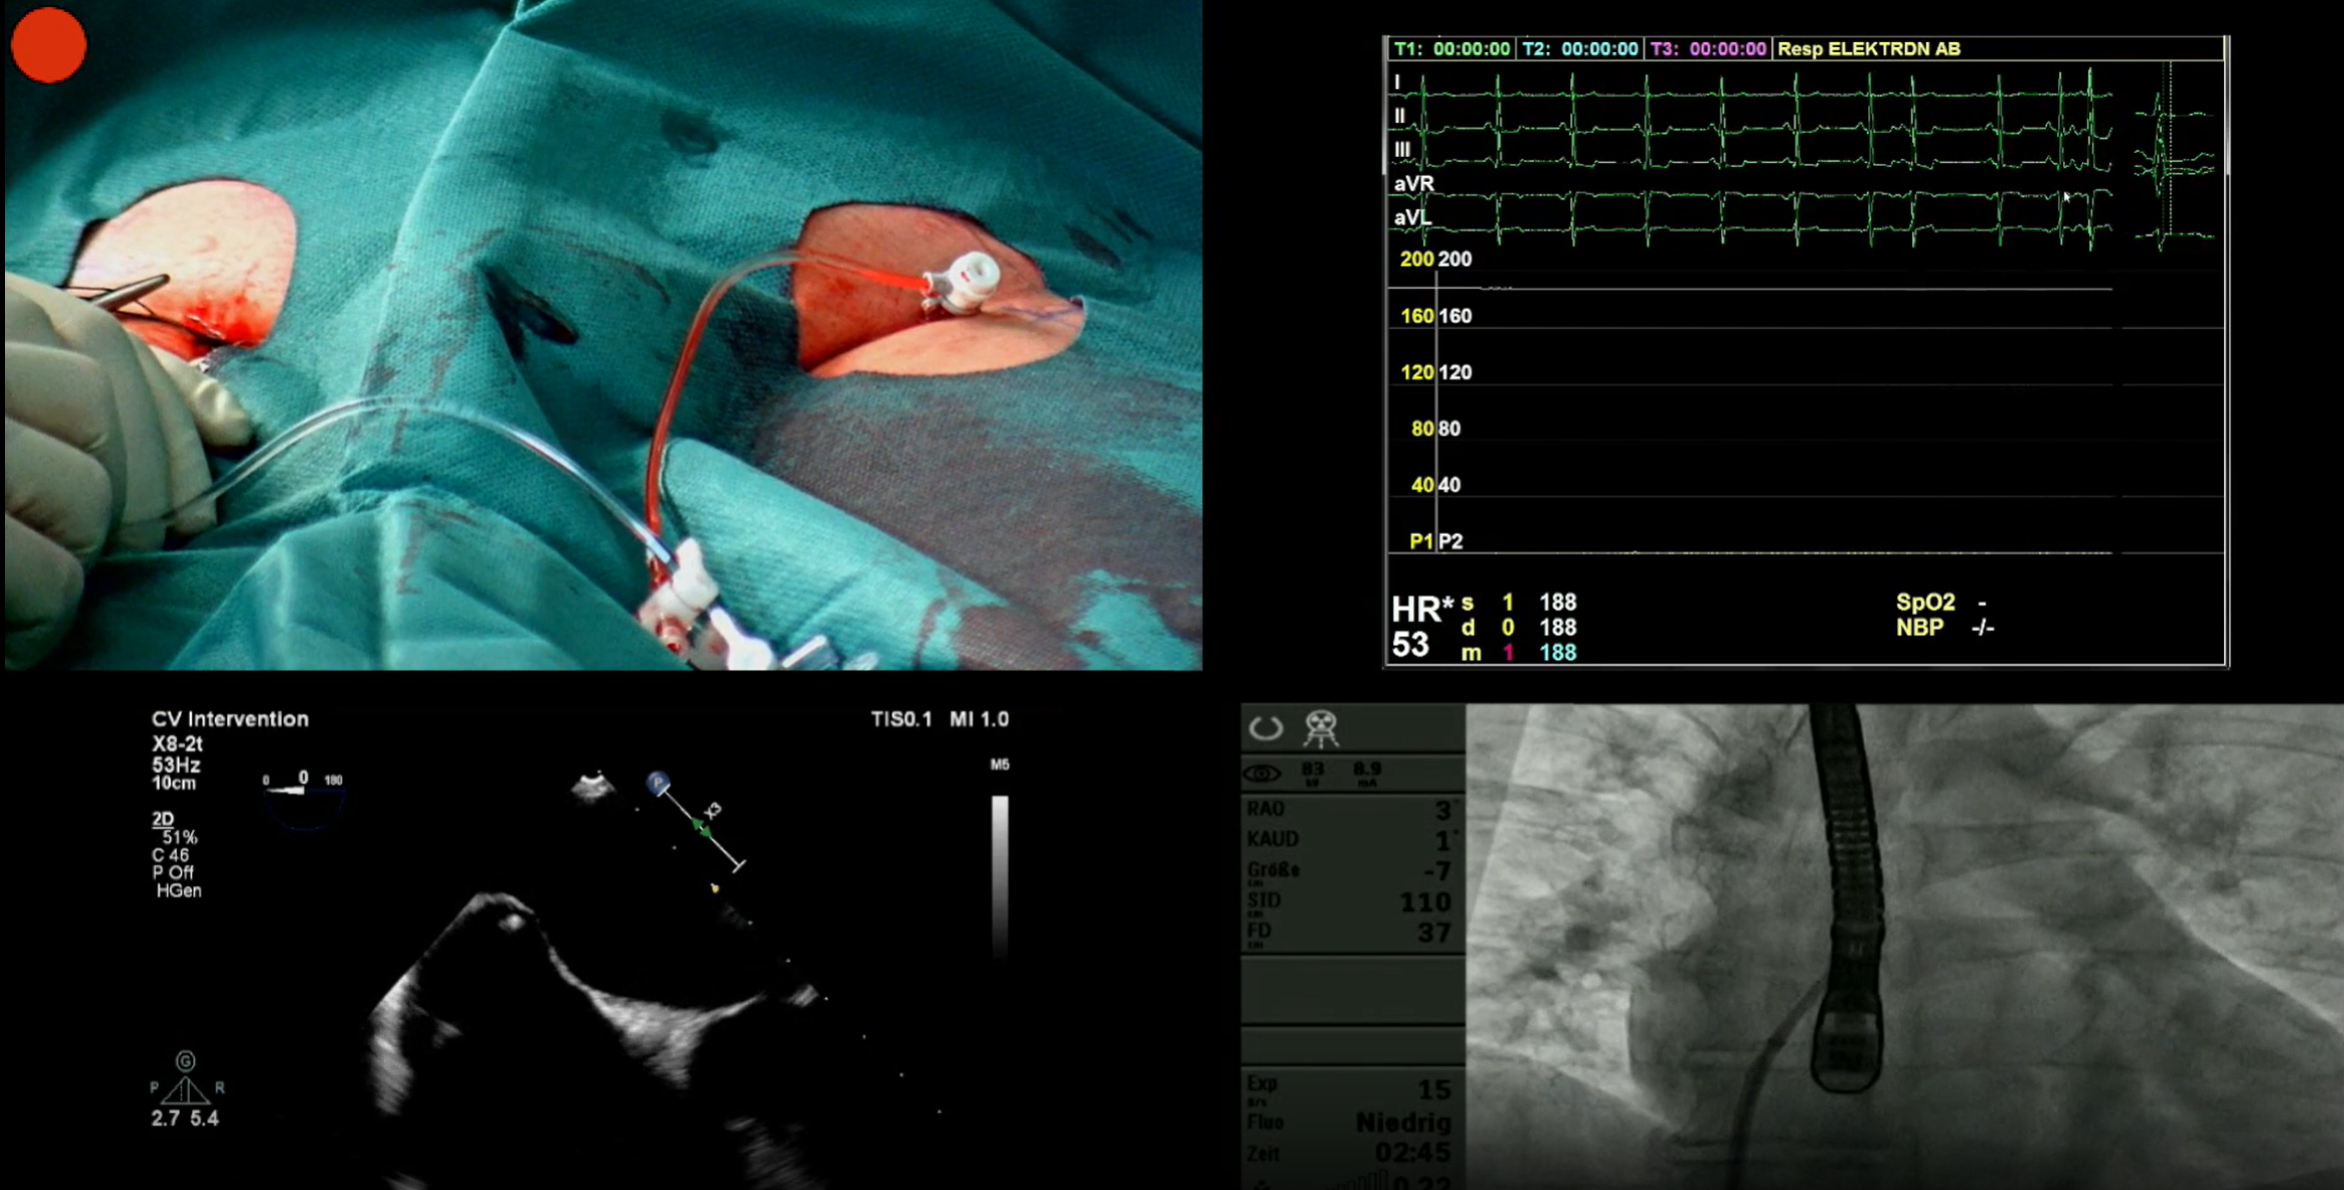
\includegraphics[width=1\linewidth]{images/teer/fig TEER TS video.png}
    \caption{關於transseptal puncture for M-TEER, Cardiac Interventions Today有錄製很清楚的影片供參考。這邊將之cite如附圖。\href{http://cf.cdn.vid.ly/2r9y9b/mp4_1080.mp4}{http://cf.cdn.vid.ly/2r9y9b/mp4_1080.mp4}}
    \label{images/teer/fig TEER TS video}
\end{figure}

% https://citoday.com/articles/2019-may-june/transseptal-puncture-a-step-by-step-procedural-guide

% to be edited: add reference and figures from: Simard2021

% training requirement for transseptal puncture: 30
% Alkhouli2016


\subsection{Insertion of steerable guide catheter (SGC)}
\subsection{Straddling}
Stradding的動作在MitraClip為重要步驟，為的是讓SGC與CDS之間的可動關結有最大活動度，且不至於造成device損壞。而PASCAL device則不需要這個步骤，因為其靈活度在設計上不用考慮SGC與CDS之間的限制。

\subsection{Adjustment for trajectory}
進行TEER最讓人覺得目眩神馳的就是operator如何操作MitraClip, TriClip, or PASCAL上面的諸多旋鈕。這些knob (旋鈕)每個都控制一個轉向或是關鍵clip/clasp構造，所以在Mainz有很大的一段時間是要弄清楚如何操作。

而Trajectory adjustment則為device enter to target valve前的重要動作之一。要確保entering to LV or RV的 trajectory 為perpendicular to valve orifice. 舉例若是central position, posterior trajectory, 應該要flex guide sheath (PASCAL) 再加上 counter-clockwise rotation of guide sheath (PASCAL). 請參考 Figure ~\ref{images/teer/fig TEER trajectory 1}以及 Figure ~\ref{images/teer/fig TEER trajectory 2}.  

\begin{figure}
    \centering
    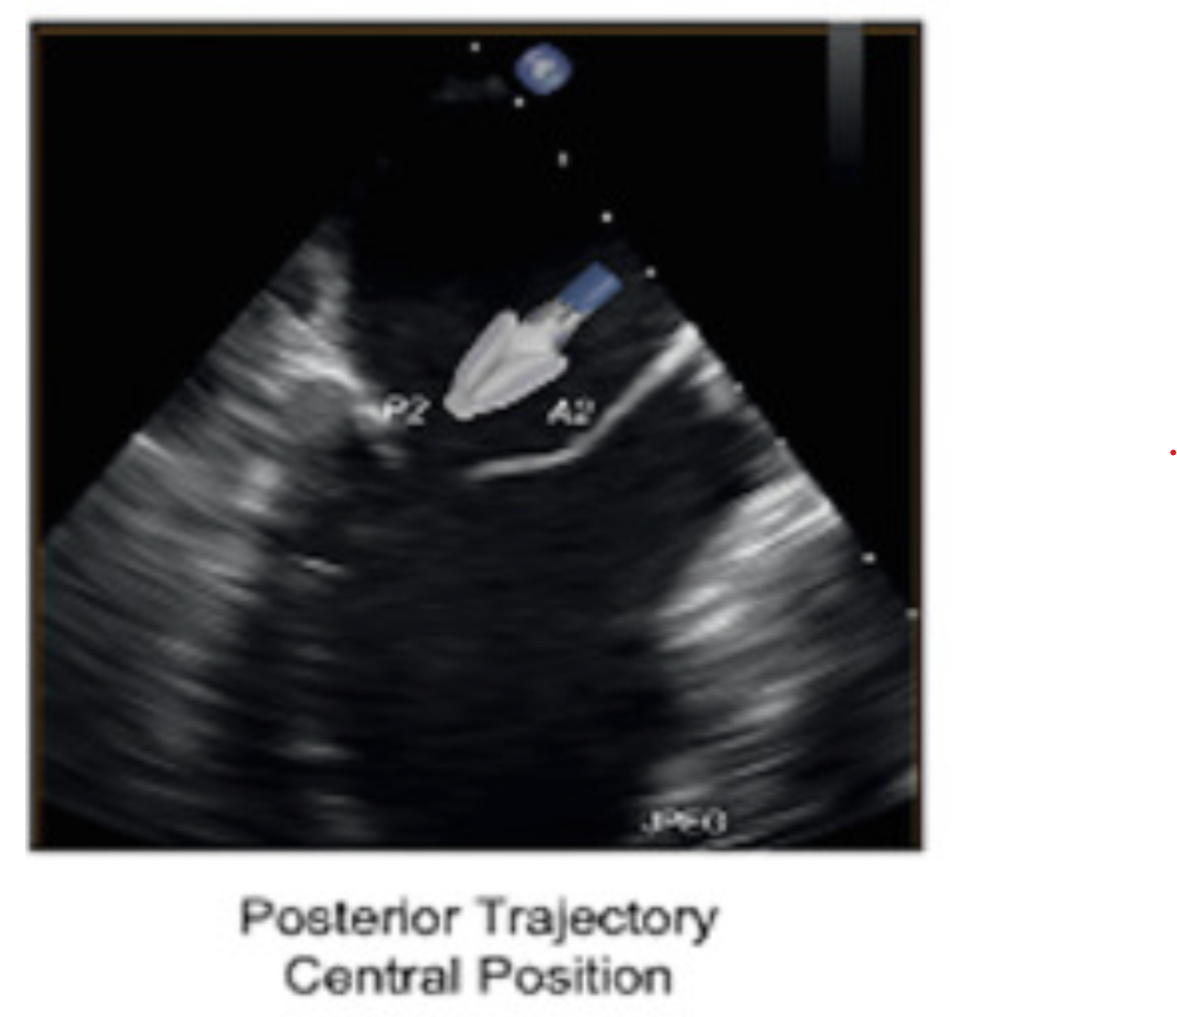
\includegraphics[width=0.9\linewidth]{images/teer/fig TEER trajectory 1.png}
    \caption{這是一個示意圖，顯示Clasp (PASCAL) tip 目前為朝後- posterior trajectory, 但是tip已經位於mitral valve orifice正中了- central position. 這時就應該要有相對應的操作，將posterior trajectory修正為central trajectory. }
    \label{images/teer/fig TEER trajectory 1}
\end{figure}

\begin{figure}
    \centering
    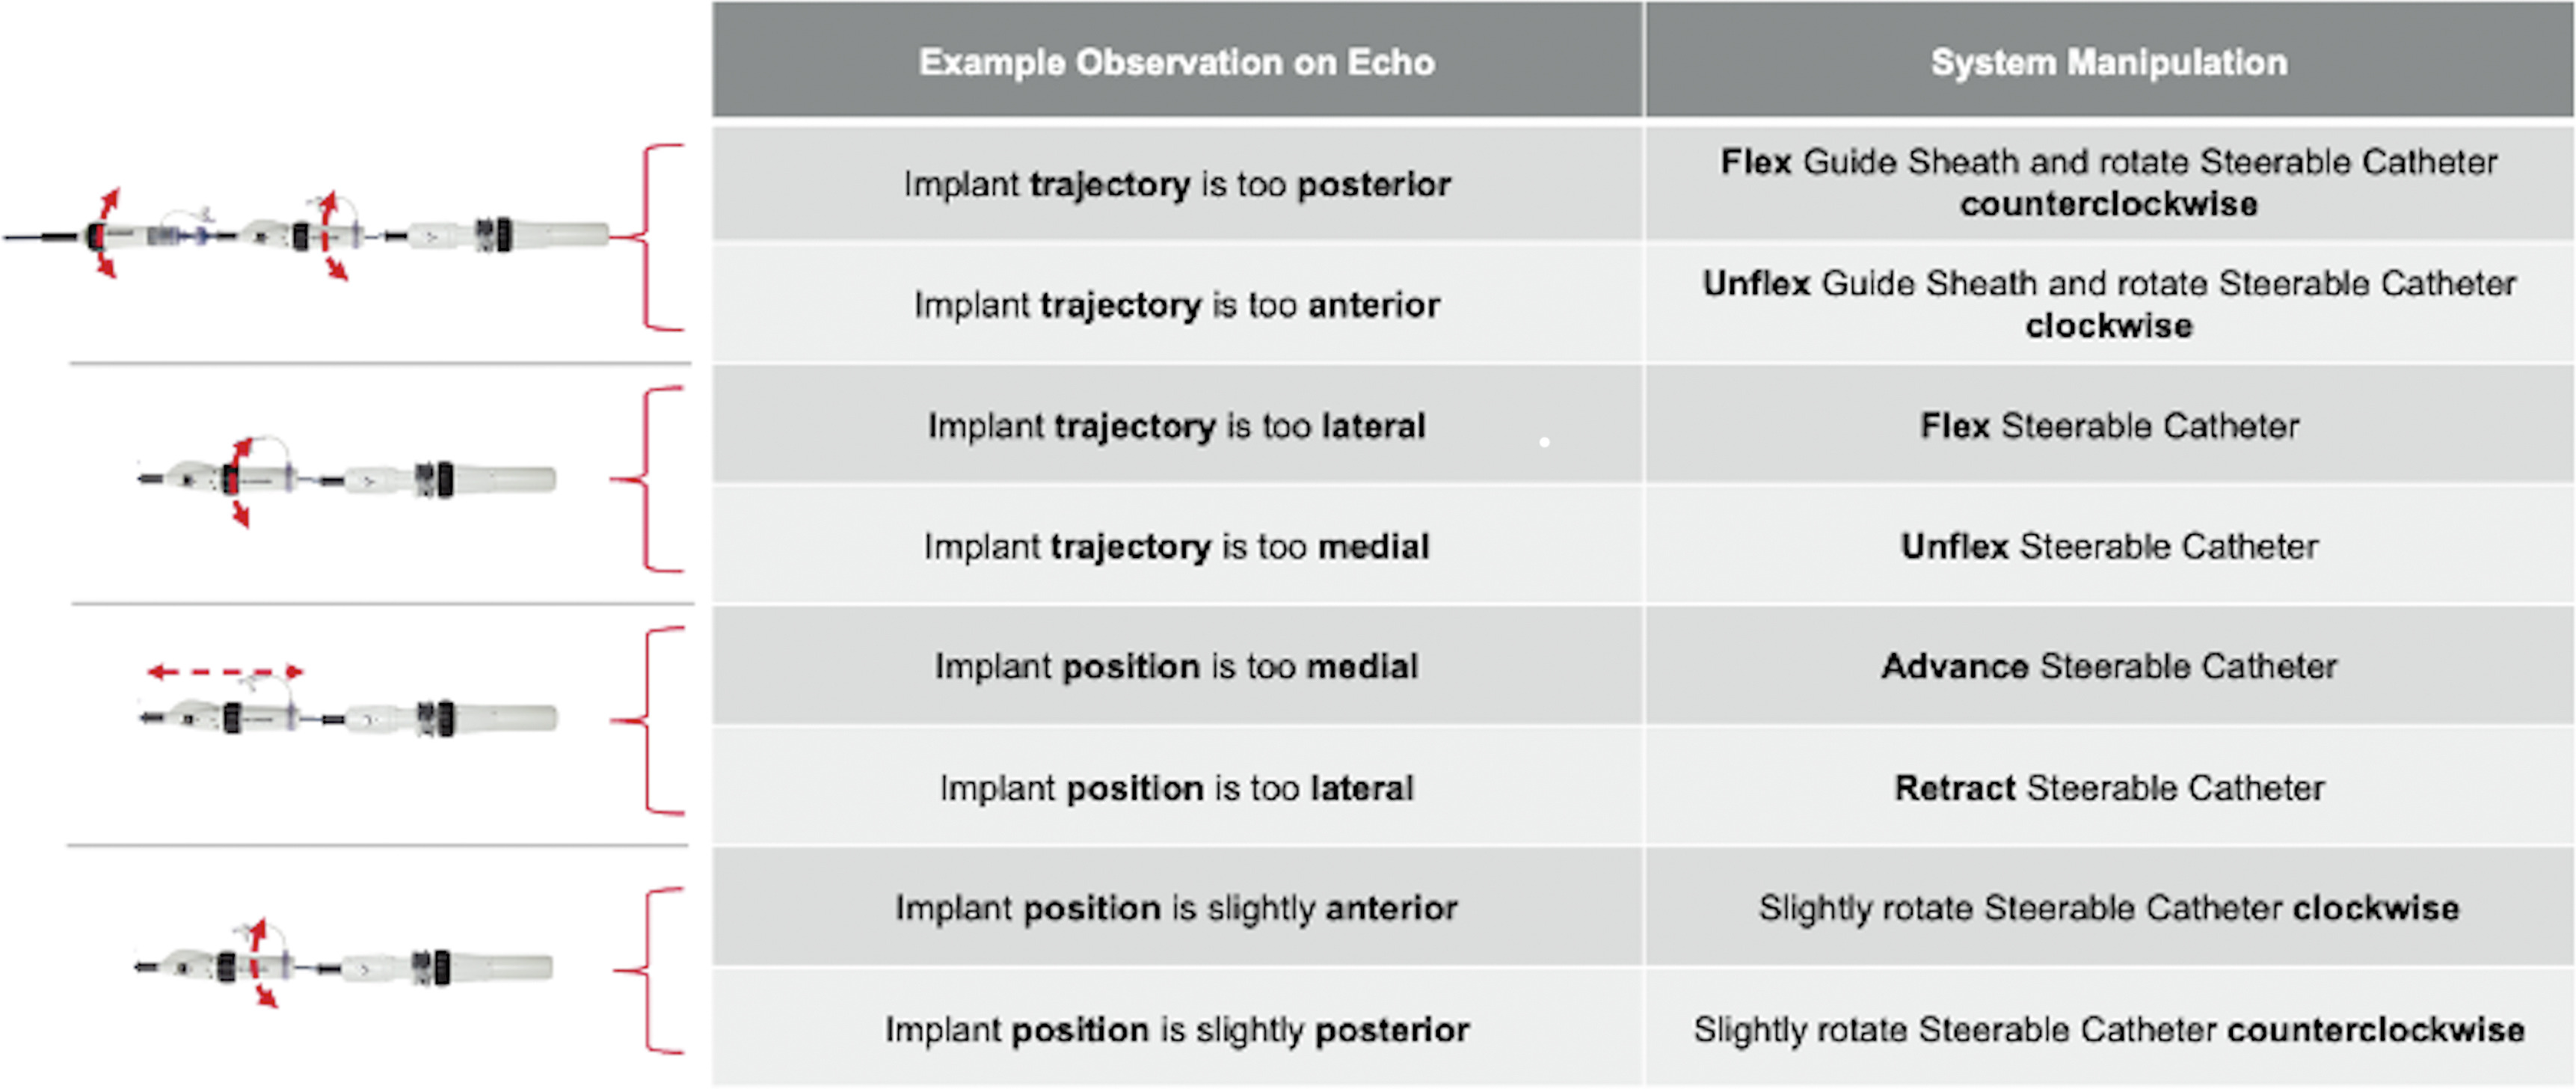
\includegraphics[width=0.9\linewidth]{images/teer/fig TEER trajectory 2.png}
    \caption{每一個相對應的trajctory and position都有操作的作法，將clip/clasp置放回正中區域。}
    \label{images/teer/fig TEER trajectory 2}
\end{figure}

操作trajectory就會需要理解，MitraClip的諸多元件，在經過transseptal puncture後，位於interatrial septum後，有哪些關結是可動的，而且與mitral valve之間的關係如何。在Figure ~\ref{images/teer/fig TEER trajectory 3}之中，可以看到軸向轉動系統與二尖瓣的關係。這張圖對於理解 steerable guide catheter (SGC), 與 catheter delivery system (CDS), 還有 clip 的前進後退，與orientation相當重要。

\begin{figure}
    \centering
    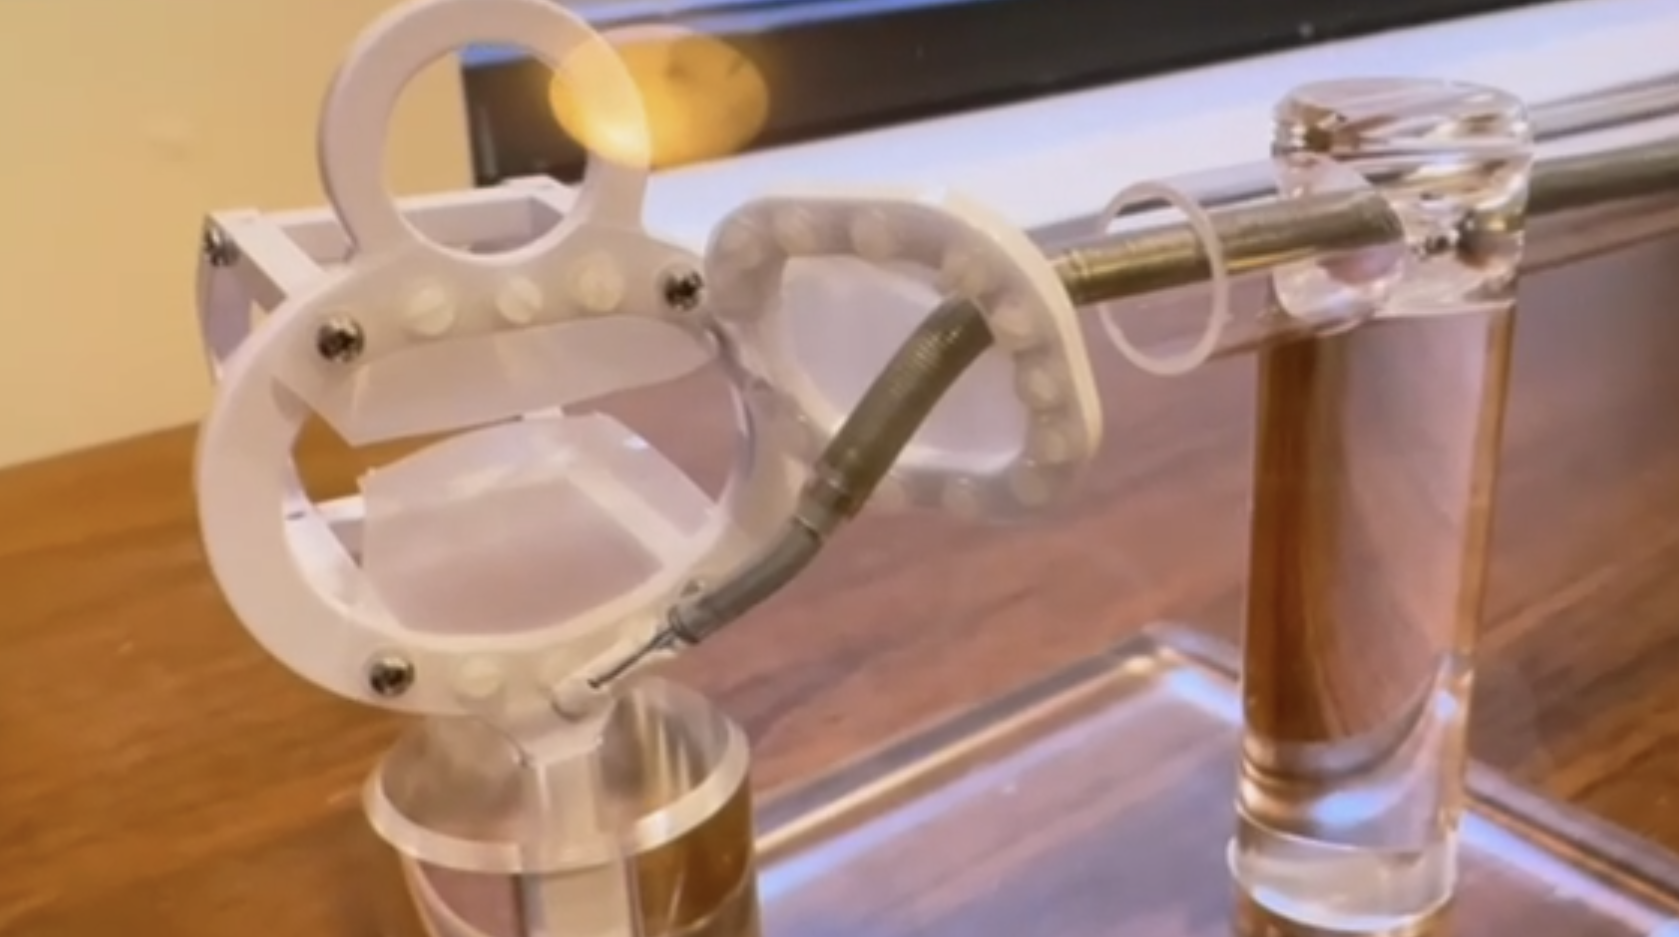
\includegraphics[width=1\linewidth]{images/teer/fig TEER trajectory 3.png}
    \caption{TEER system有許多可動關節與構造，圖片以MitraClip為例，顯示steerable guide catheter (SGC), catheter delivery system (CDS), clip and orientation之間的關係。}
    \label{images/teer/fig TEER trajectory 3}
\end{figure}

測定與調整 trajectory, 都會需要在TEE的兩個panels螢幕上看清楚anterior-posterior以及medial-lateral (Figure ~\ref{images/teer/fig TEER trajectory 4}). 



\begin{figure}
    \centering
    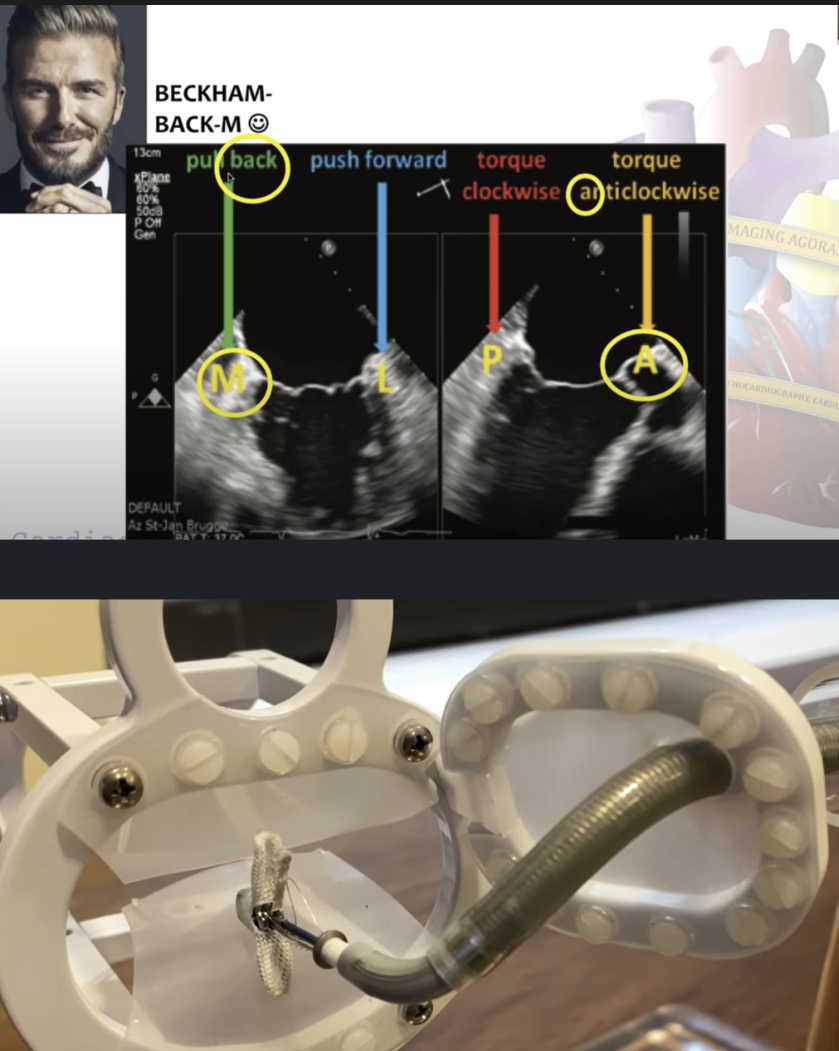
\includegraphics[width=0.8\linewidth]{images/teer/fig TEER trajectory 4.png}
    \caption{MitraClip的M-L knob, 需要看TEE monitor左側的panel, 弄清楚intercommissural plane上面clip與mitral valve之間的相對關係。}
    \label{images/teer/fig TEER trajectory 4}
\end{figure}

\subsection{Check gripper and adjustment for orientation}
在這一步，要確定clip/clasp兩個可以單獨抓取mitral leaflet的單元在空間上的對應，更要確定clip/clasp的方向是與leaflet coaptation line保持垂直的 (Figure ~\ref{images/teer/fig TEER trajectory 4})。Figure ~\ref{images/teer/fig TEER orientation 1}顯示的是標準的A2/P2 grasping orientation. 

\begin{figure}
    \centering
    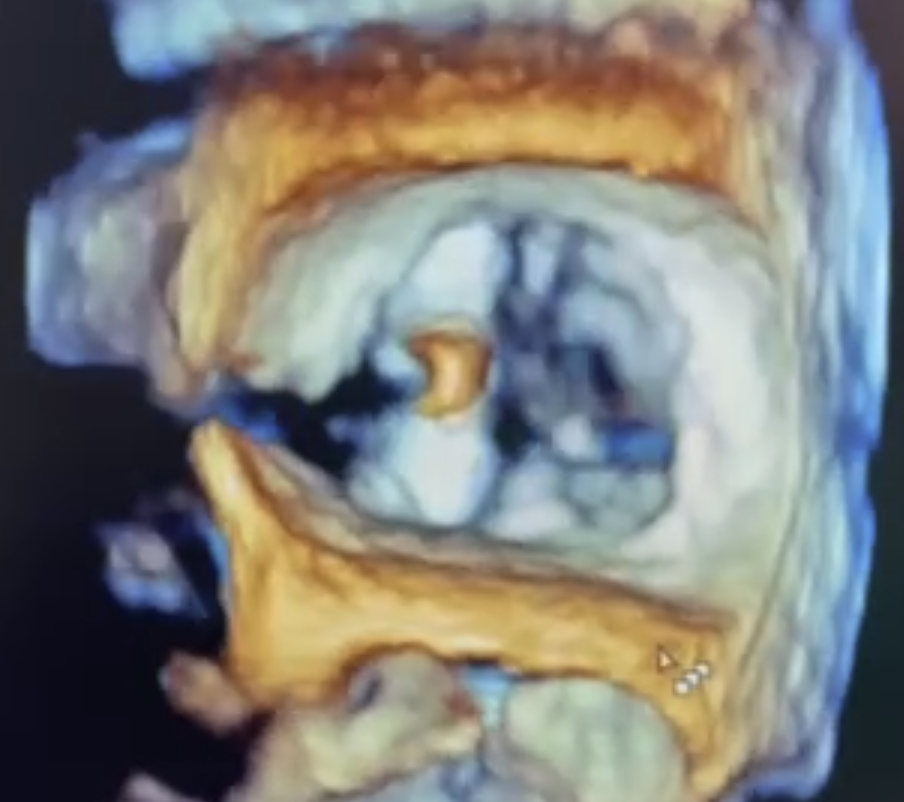
\includegraphics[width=0.75\linewidth]{images/teer/fig TEER orientation 1.png}
    \caption{此為 clocking (orientation)中，clip的方向為 12-6點鐘，針對 grasping zone: A2-P2是perpendicular垂直於leaflet coaptation, 所以是標準的 orientation (clocking) for A2/P2. 圖中aorta在6點鐘方向 (Mainz standard view)。}
    \label{images/teer/fig TEER orientation 1}
\end{figure}

\subsection{Leaflet grasping}
這一步是所有動作裡，花費時間最多的一步，因為要等待TEE的影像調整到最佳，然後lower-down gripper後，然後評估抓取前後的leaflet insertion是否足夠，才再把clip/clasp關上 (Figure ~\ref{images/teer/fig TEER leaflet grasping})。之後再進行color mapping, post-clipping echo evaluation (Figure ~\ref{images/teer/fig TEER leaflet color evaluation}). 

\begin{figure}
    \centering
    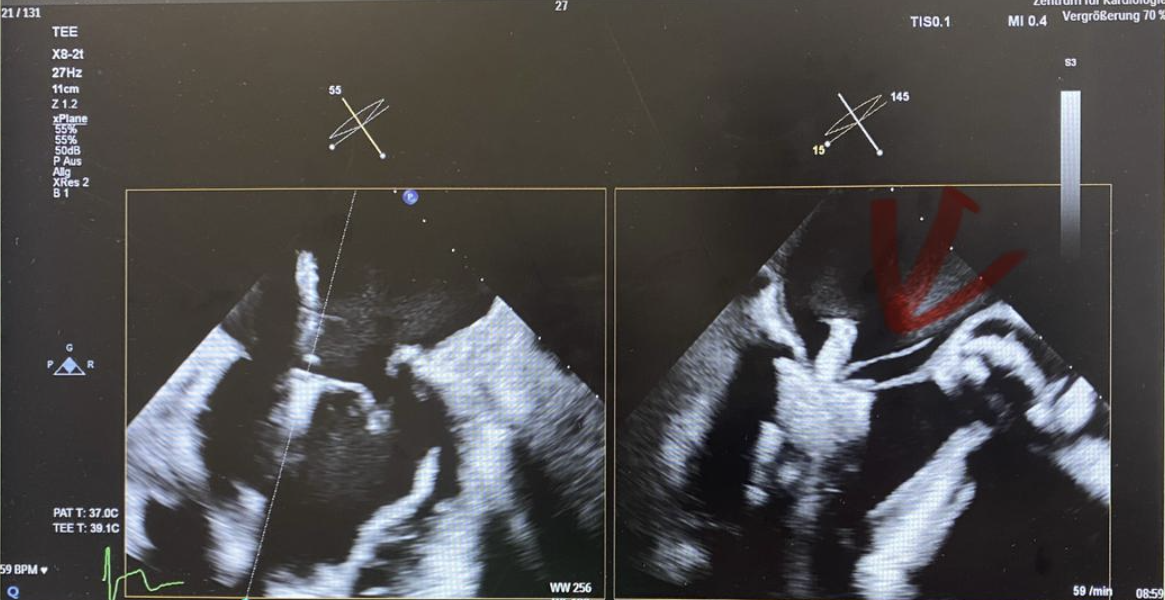
\includegraphics[width=1\linewidth]{images/teer/fig TEER leaflet grasping.png}
    \caption{瓣葉的抓取 (grasping) 對於影像判斷，操作技巧有極大的要求，其中判斷的重點是: leaflet becomes immobile. 這張圖裡面，病患有congenital anomaly: congenital cord extending from anterior leaflet to inter-atrial septum. }
    \label{images/teer/fig TEER leaflet grasping}
\end{figure}


\begin{figure}
    \centering
    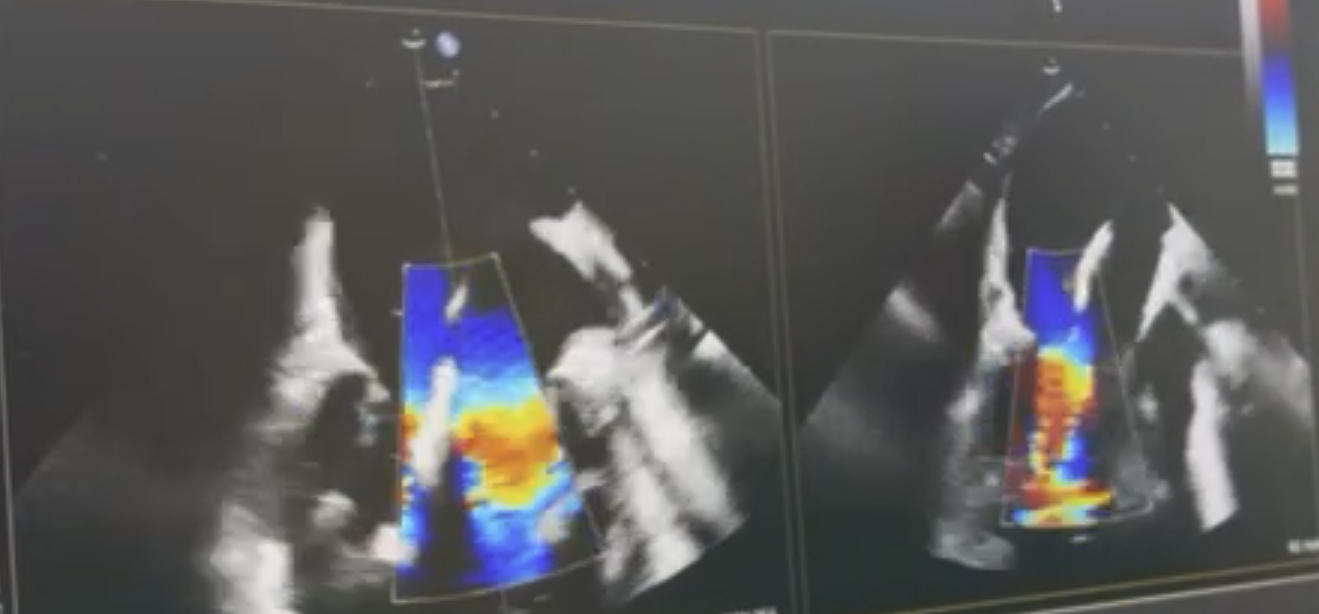
\includegraphics[width=1\linewidth]{images/teer/fig TEER leaflet color evaluation.png}
    \caption{抓取葉片後，關上clip/clasp, 就會依序完成 color mapping評估，mitral valve area 重新評估，change in pulmonary flow pattern, 以及hemodynamics再評估。}
    \label{images/teer/fig TEER leaflet color evaluation}
\end{figure}


\subsection{Final deploy}


\begin{longtable}{p{1cm} p{10cm}}
\caption{MitraClip/TriClip deploy時的操作，請參考Figure\ref{images/teer/fig MitraClip system}的標示。}
\hline
\textbf{步驟} & \textbf{說明} \\ \hline
\endfirsthead
\hline
\textbf{步驟} & \textbf{說明} \\ \hline
\endhead
\hline
\endfoot
1 & 從 locker 處抽線，要轉開 lock 的透明旋蓋，拉出像糖果紙一樣的包裝，然後把線的一端完全拉出。 \\ \hline
2 & 拉線拉完後，轉白色的 clip arm positioner。先逆時針（CCW, counter-clockwise rotation）轉，確定在 lock 的情況下不能再打開 clip，然後順時針（CW, clockwise rotation）轉，將其鎖死。 \\ \hline
3 & 逆時針（CCW）轉 clip arm positioner 到 neutral position，確保沒有鬆也沒有緊。 \\ \hline
4 & 拉出插梢。 \\ \hline
5 & 繼續逆時針轉鬆 clip arm positioner。 \\ \hline
6 & 鬆開 CDS 的黑色小固定旋鈕。 \\ \hline
7 & 轉動銀色 cone。 \\ \hline
8 & 部署（Deploy） clip。 \\ \hline
9 & 拉開 gripper。 \\ \hline
10 & 退出 CDS，然後退出 SGC。 \\ \hline
11 & 縫合傷口（suture）。 \\ \hline
\end{longtable}

\begin{figure}
%\vskip -1.2in
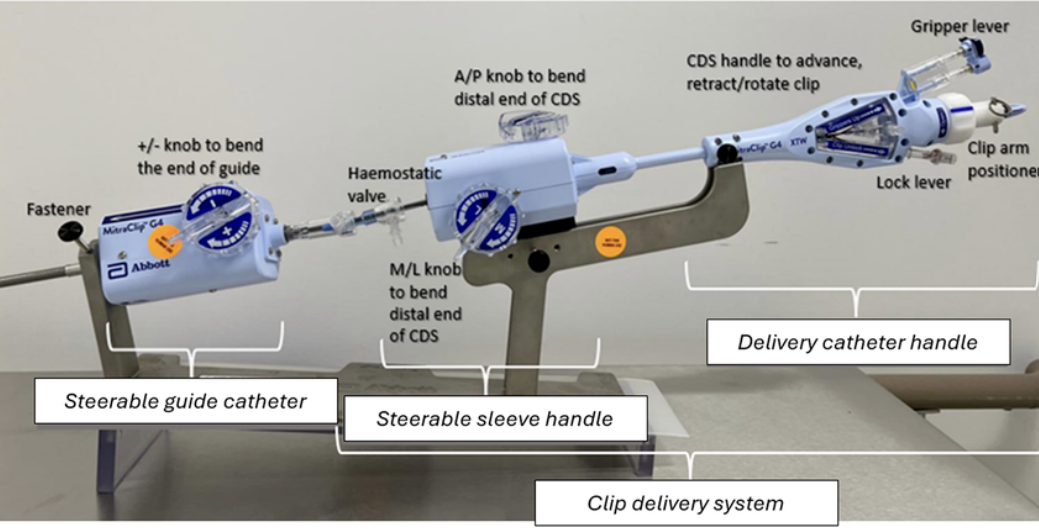
\includegraphics{images/teer/fig MitraClip system.png}
\caption{Deploy clip之前要作的一系列動作，請參考system構造元件名稱。}
\label{images/teer/fig MitraClip system}        
\end{figure}

\newpage

\section{Post-procedure TEE cleaning}
清消有特別盒子，並且用兩層塑膠袋分隔 (Figure \ref{fig TEE packaging})。

\begin{figure}
    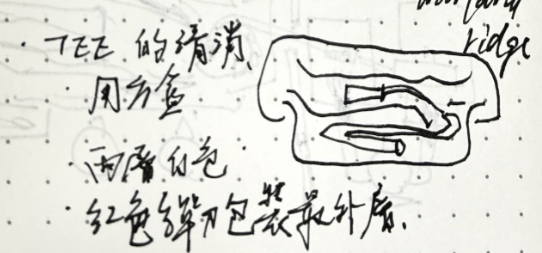
\includegraphics[width=0.75\linewidth]{images/teer/fig TEE cleaning.png}
    \caption{TEE的清消，在術後均以圖示方式包裝，有效率，且可達到足夠的感染隔離。}
    \label{fig TEE packaging}
\end{figure}


\section{Shock after TEER}
TEER執行後若病人發生shock要怎麼辦? 
立刻用TEE直接評估是否有新的pericardial effusion或是new regoinal wall motion abnormality, 以及是否有iatrogenic mitral stenosis. 
以下為重要鑑別診斷，不論是否為 mitral-TEER or tricuspid-TEER: 
\begin{itemize}
    \item Aortic stenosis
    \item Aortic regurgitation
    \item Tricuspid regurgitation
    \item ASD-related Rt to Lt shunting- associated with severe TR
    \item Infiltrative cardiomyopathy
    \item LCX compromise, due to significant force exerted by the clip
    \item RV failure
\end{itemize}

\section{Post-TEER echocardiography follow-up}

要用TEE評估下面事項:
\begin{itemize}
    \item jet color mapping area
    \item mitral and tricuspid inflow velocity and mean pressure gradient (M-TEER mitral inflow mean PG should < 5 mmHg)
    \item mitral valve area: should > 1.5 cm$^2$
    \item tricuspid valve area: should > 2.5 cm$^2$   
\end{itemize}

%\cite{Zoghbi2019}
\begin{figure}
    \centering
    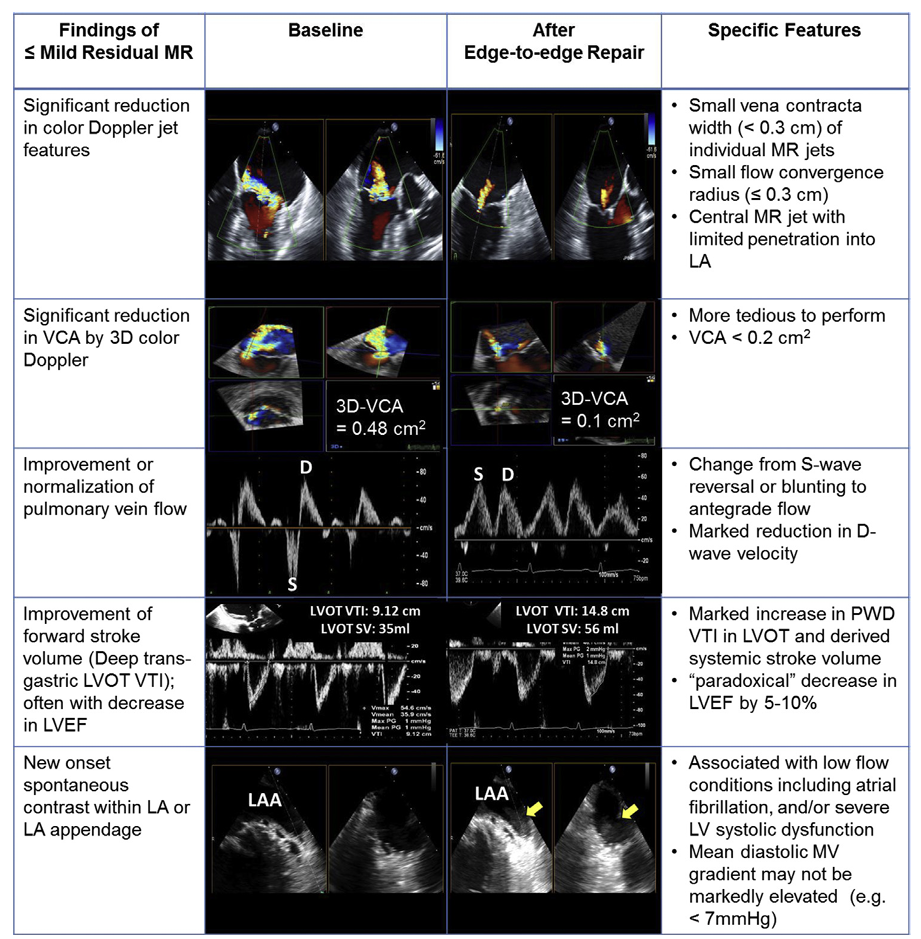
\includegraphics[width=\linewidth]{images/teer/fig TEER echo follow.png}
    \caption{減少二尖瓣關閉不全（MR）嚴重程度至輕微的TEER results.}
    \label{images/teer/fig TEER echo follow}
    
\end{figure}

\clearpage
\section{Reporting standards- 如何完成一份 TEER 報告}
\subsection{德國Mainz的正式報告}
以下為去辨識資料，可以看到德國報告的格式。
\begin{figure}
    \centering
    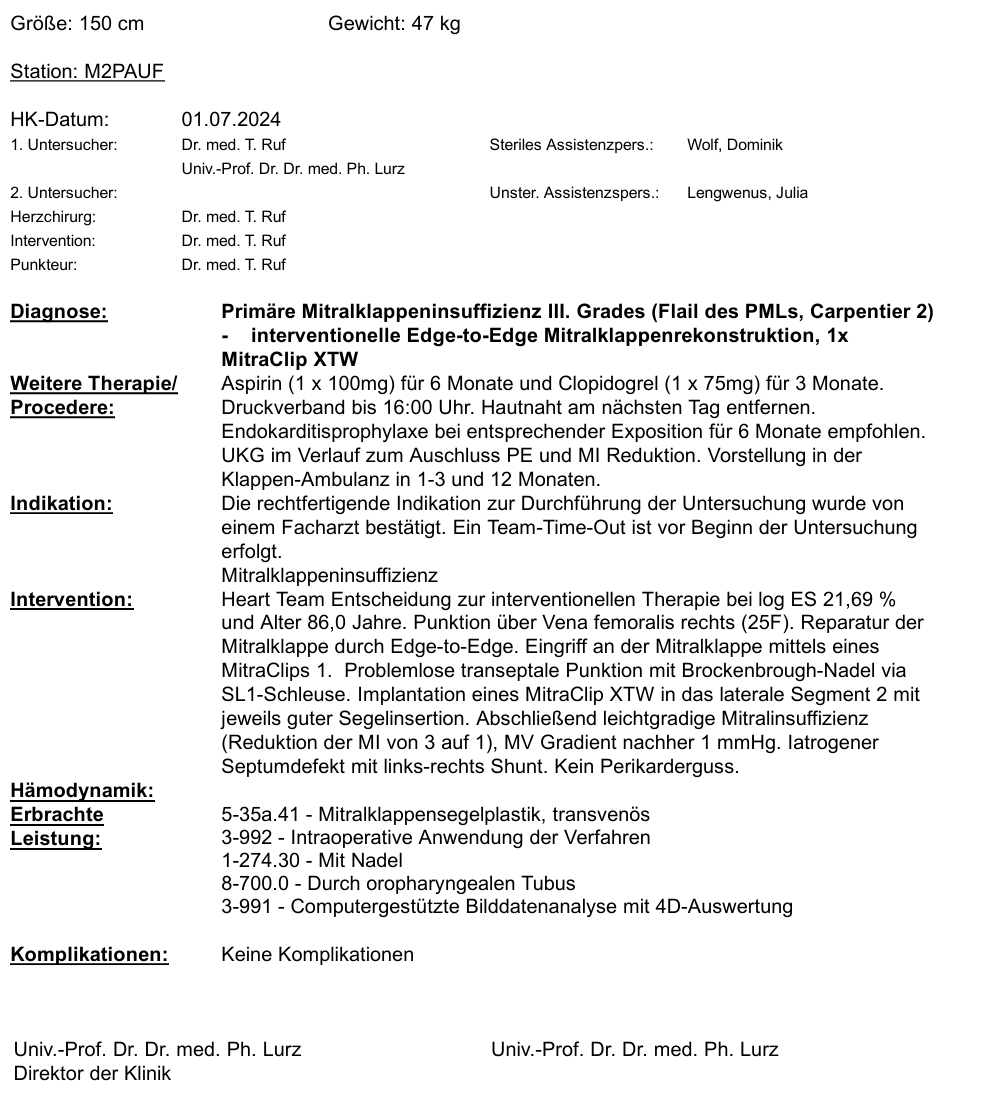
\includegraphics[width=1\linewidth]{images/teer/fig TEER reporting example 2.png}
    \caption{以下為去辨識資料，可以看到德國報告的格式}
    \label{images/teer/fig TEER reporting example 2}
\end{figure}


打在導管報告系統中，我們新竹內建的導管系統，有一區是完全空白，是可以打術式細節與內容在其中的。

\begin{figure}
    \centering
    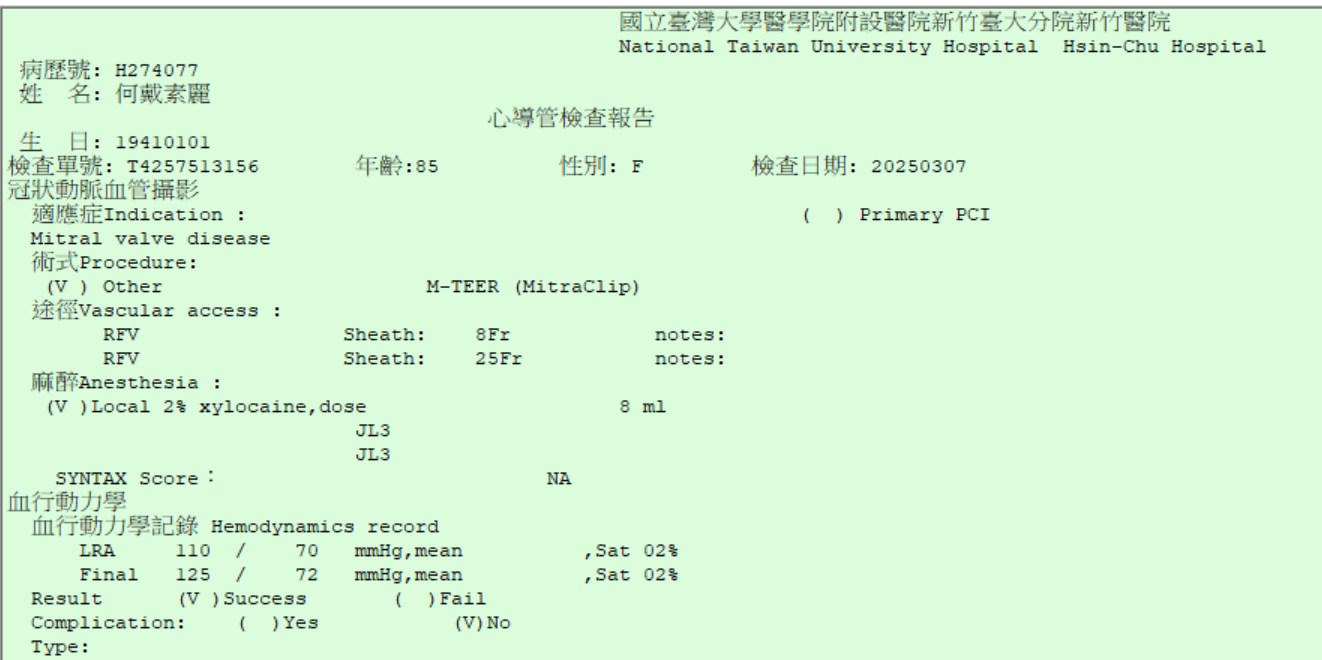
\includegraphics[width=0.75\linewidth]{images/teer/fig TEER reporting screen.png}
    \caption{導管報告書寫格式規範}
    \label{images/teer/fig TEER reporting}
\end{figure}

\subsection{Example of a TEER report}
下面是一份範例報告，依照 Mainz, Germany formal report 參考完成。
病人為2025-03-07的病患。

\begin{figure}
    \centering
    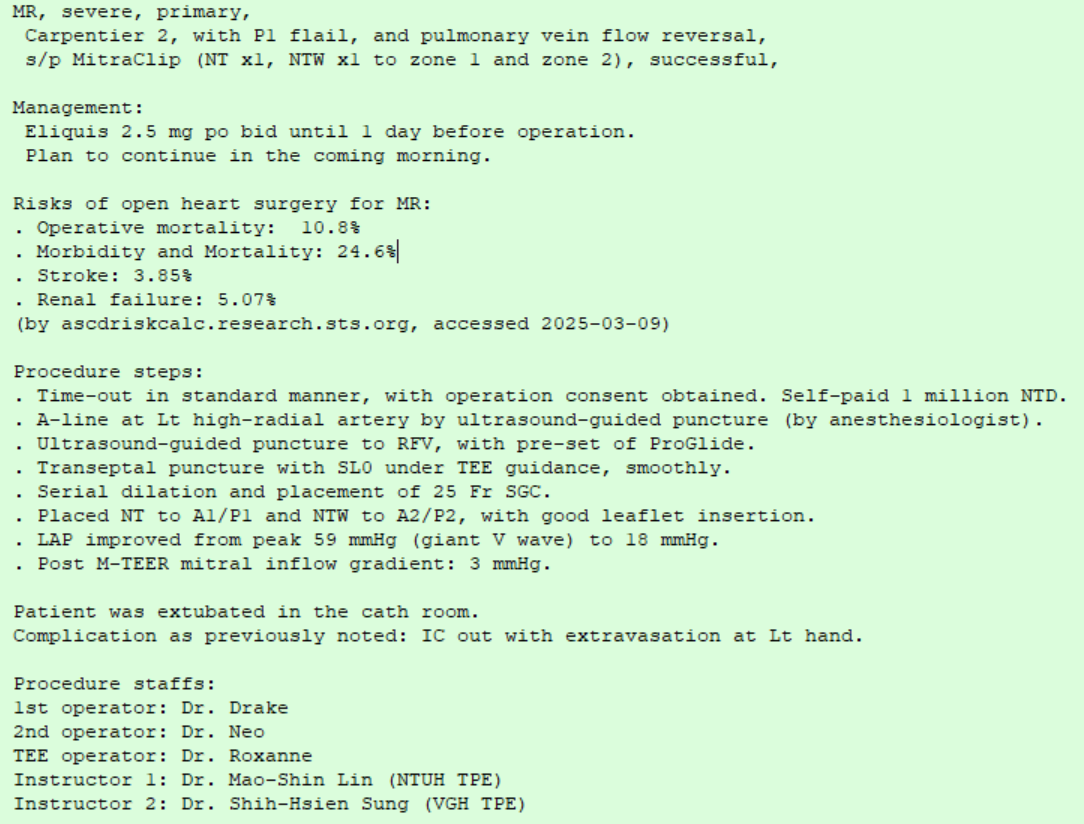
\includegraphics[width=1\linewidth]{images/teer/fig TEER reporting example 1.png}
    \caption{報告範例，請注意裡面的 Risks of open heart surgery for MR是由標準STS score算出來的結果，呈現在我們的報告中，請參考 Fig ~\ref{images/general/fig surgical risk calculator}}
    \label{images/teer/fig TEER reporting example 1}
\end{figure}

\textbf{MR, severe, primary,\\
Carpentier 2, with P1 flail, and pulmonary vein flow reversal,\\
s/p MitraClip (NT x1, NTW x1 to zone 1 and zone 2), successful. \\}


Management:\\
Eliquis 2.5 mg po bid until 1 day before operation.\\
Plan to continue in the coming morning.\\
\\
Risks of open heart surgery for MR:\\
\begin{itemize}
\item Operative mortality: 10.8\%
\item Morbidity and Mortality: 24.6\%
\item Stroke: 3.85\%
\item Renal failure: 5.07\%
\end{itemize}
(by ascdriskcalc.research.sts.org, accessed 2025-03-09)\\
\\
Procedure steps:\\
\begin{itemize}
\item Time-out in standard manner, with operation consent obtained. Self-paid 1 million NTD.
\item A-line at Lt high-radial artery by ultrasound-guided puncture (by anesthesiologist).
\item Ultrasound-guided puncture to RFV, with pre-set of ProGlide.
\item Transeptal puncture with SLO under TEE guidance, smoothly.
\item Serial dilation and placement of 25 Fr SGC.
\item Placed NT to A1/P1 and NTW to A2/P2, with good leaflet insertion.
\item LAP improved from peak 59 mmHg (giant V wave) to 18 mmHg.
\item Post M-TEER mitral inflow gradient: 3 mmHg.
\end{itemize}
\\
Patient was extubated in the cath room.\\
Complication as previously noted: IC out with extravasation at Lt hand.\\
\\
Procedure staffs:\\
\begin{itemize}
    \item 1st operator: Dr. Drake
    \item 2nd operator: Dr. Neo
    \item TEE operator: Dr. Roxanne
    \item Instructor 1: Dr. Mao-Shin Lin (NTUH TPE)
    \item Instructor 2: Dr. Shih-Hsien Sung (VGH TPE)
\end{itemize}

\subsection{Risk documentation- 如何計算並登錄病患operative risks}
到網站:https://acsdriskcalc.research.sts.org/ 輸入資料後，可以取得 STS risk score. 在畫面的右上與右下可以copy然後將資料貼進報告與病程記錄中 (按 copy 鈕)。

在這個範例中，病患的 operative mortality 是 10.8\%. 

\begin{figure}
    \centering
    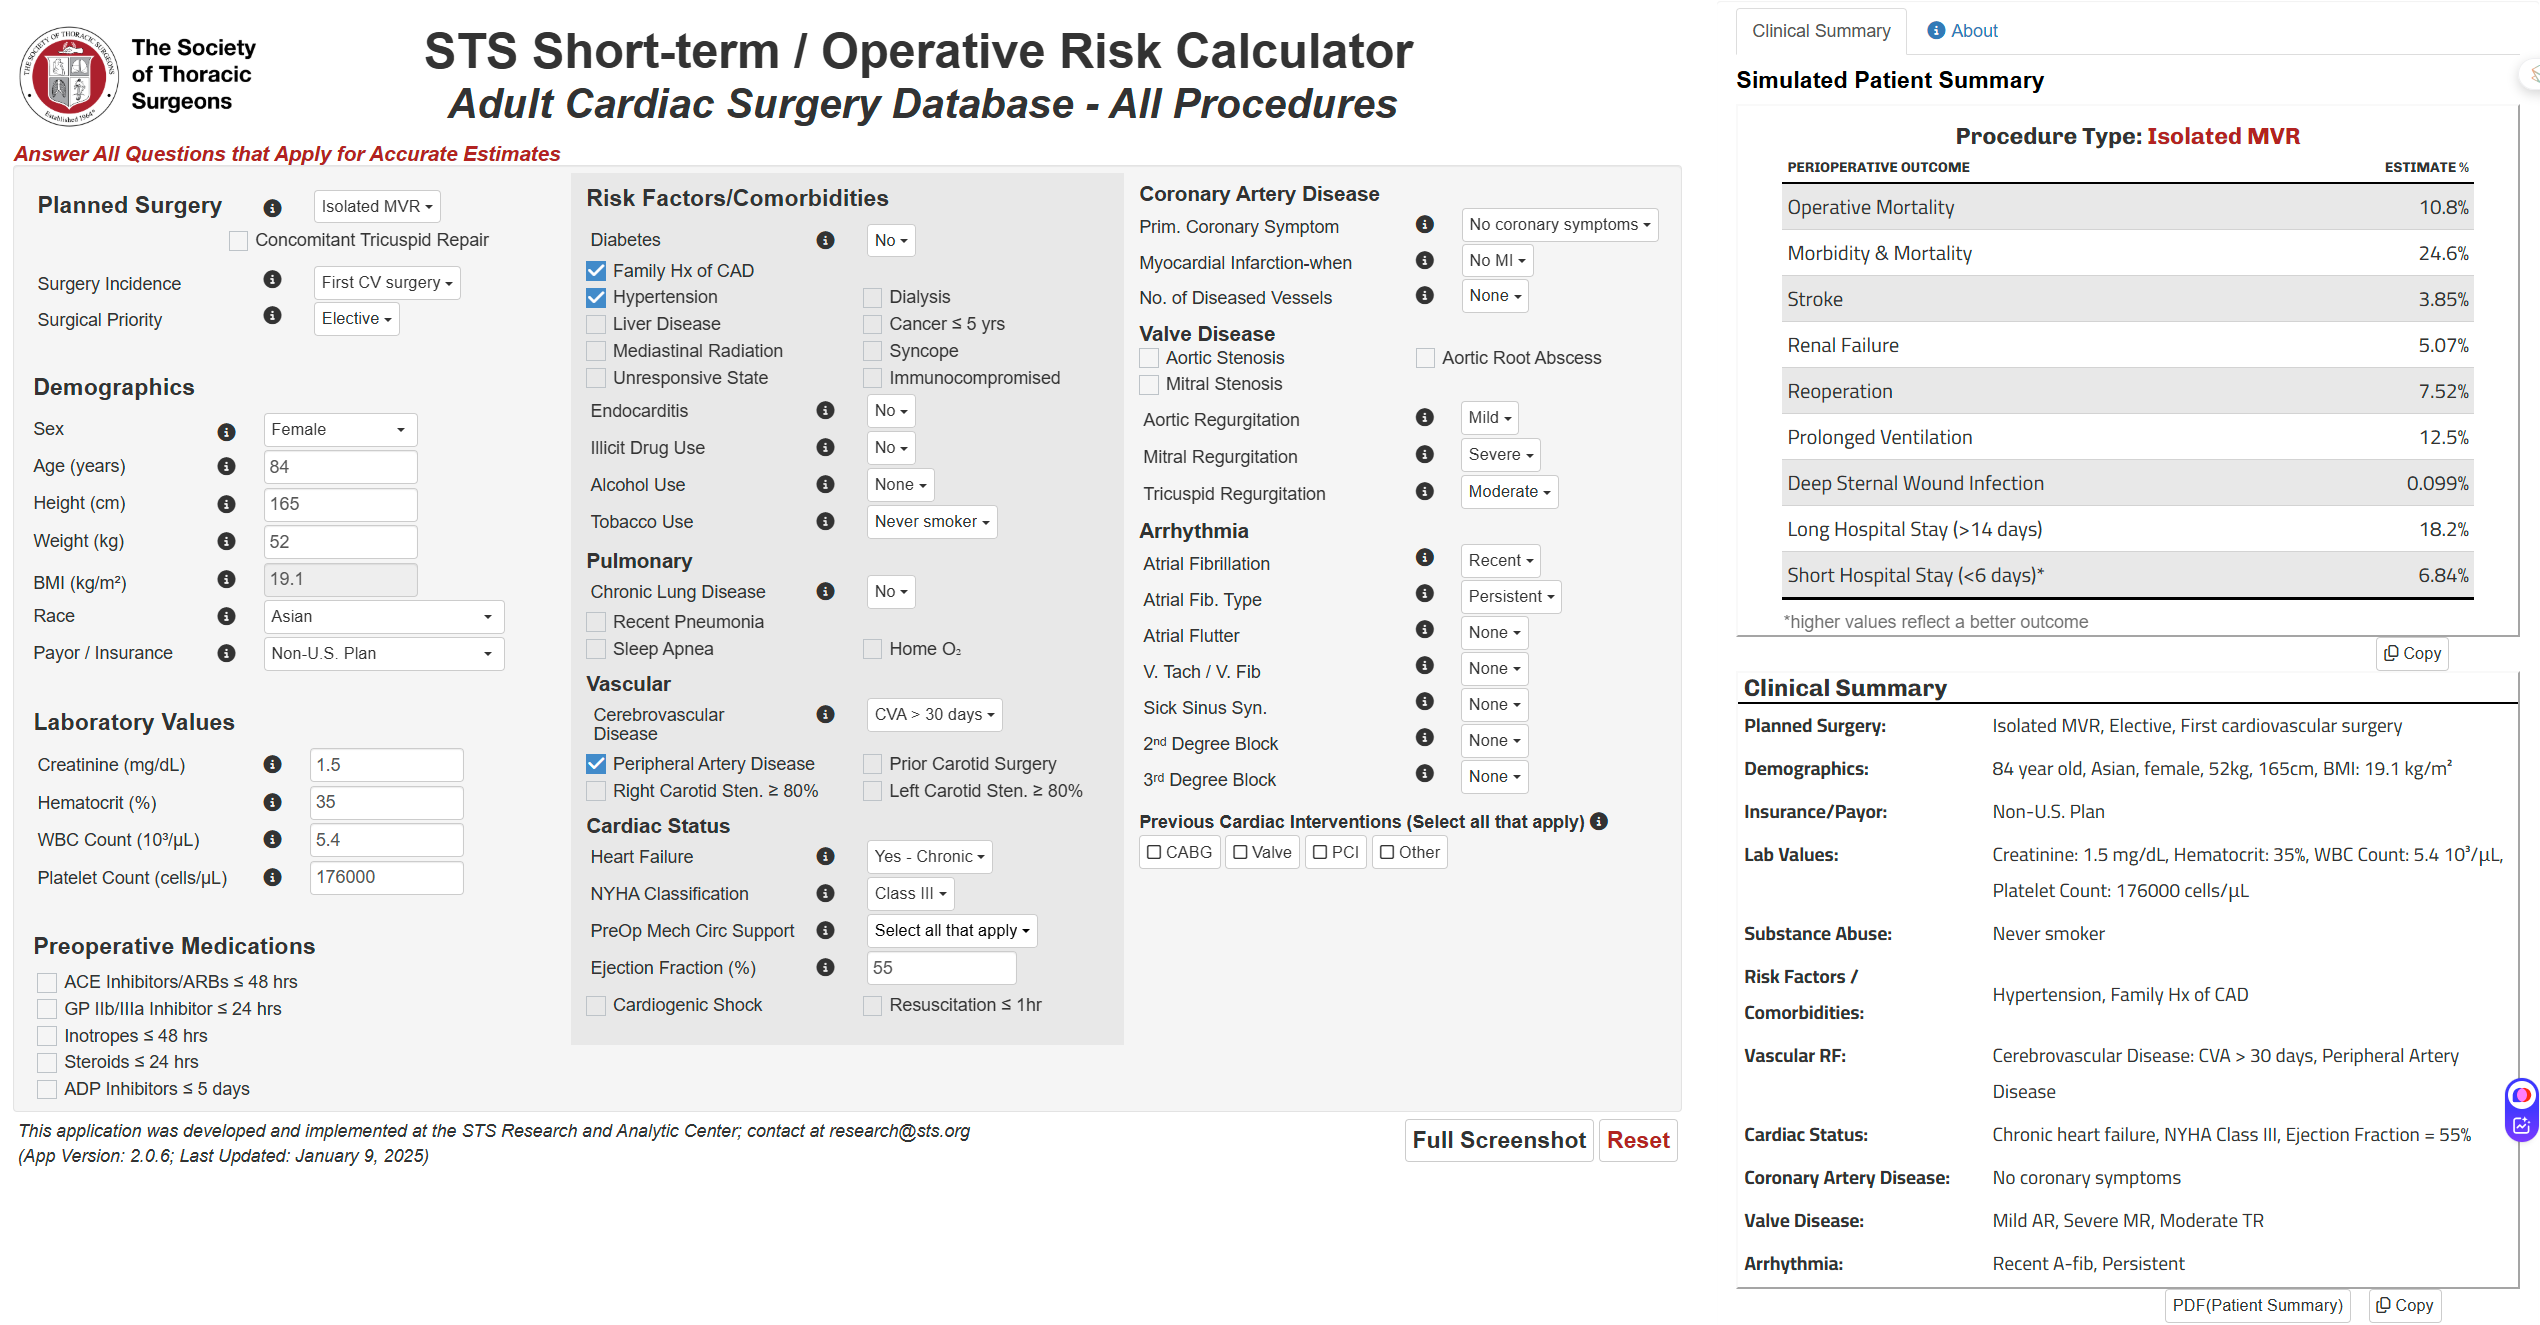
\includegraphics[width=1\linewidth]{images/general/fig surgical risk calculator.png}
    \caption{在這個範例中，病患的 operative mortality 是 10.8\%. 可以在 Fig ~\ref{images/teer/fig TEER reporting example 1}看到operative mortality: 10.8\%呈現在報告中。}
    \label{images/general/fig surgical risk calculator}
\end{figure}




\chapter{TAVI in AS}

\section{Patient selection for TAVI in AS}
TAVI in AS 適應症：

\begin{enumerate}
    \item 患者有症狀性的重度主動脈狹窄（symptomatic AS）
    \item 患者的手術風險為極高、高度或中度
\end{enumerate}

其中重要指標為: 病患有重度主動脈狹窄（AS），且有症狀和/或左心室（LV）收縮功能異常（即 LVEF < 50\%）。


重度主動脈狹窄的標準：
high gradient AS 定義為經CW (continuous wave)測量的平均跨瓣壓力梯度 (trans-valvular mean pressure gradient) ≥ 40 mmHg 或主動脈射流速度 (trans-valvular peak velocity) $\geq$ 4 m/s. 


\subsection{MDCT and fluoroscopy-guidance}
% Theriault2014 shows the importance of optimal projection curves for TAVI intervation


\section{Pre-TAVI evaluation by MDCT}
MDCT具有預測下面併發症的能力\cite{Soon2017, Adamo2019}: 
% Soon2017:  Multimodality Imaging for Planning and Follow-up Transcatheter Aortic Valve Replacement

\begin{figure}
  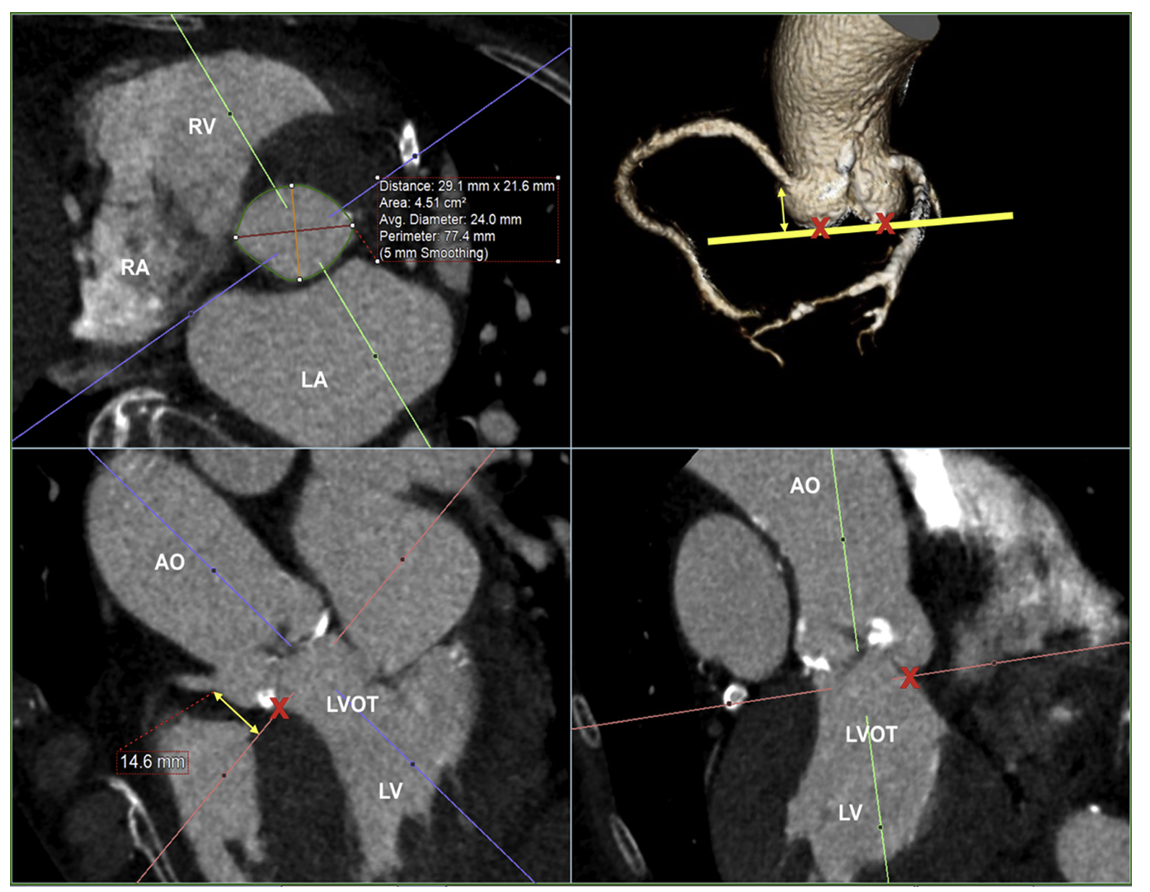
\includegraphics[width=\linewidth]{images/tavi/fig TAVI MDCT.png}
  \caption{使用多層電腦斷層掃描（MDCT）進行多平面和三維重建測量主動脈瓣環。Aortic annular plane 由虛擬基底平面（粗黃色線）定義，連接每個主動脈瓣葉的hinge points（紅色 X，標記左冠狀瓣和右冠狀瓣）。在橫向軸位圖像（右上圖）中的測量顯示瓣環面積為 4.51 cm$^2$，周長 (perimeter)為 77.4 mm。Sagittal oblique圖像（右下圖）可用於測量瓣環平面與右冠狀動脈開口之間的垂直距離 (coronary height)，此處為 14.6 mm. 縮寫：AO 為主動脈，LA 為左心房，LV 為左心室，LVOT 為左心室流出道，RA 為右心房，RV 為右心室。\cite{Soon2017}}
  \label{images/tavi/fig TAVI MDCT}
\end{figure}

\begin{itemize}
    \item para-valvular leak
    \item coronary acute closure
    \item aortic annular rupture
    \item AV block leading to PPM implantation
    \item vasscular complications
\end{itemize}

\subsection{Acute coronary occlusion after TAVI}
儘管發生率較低，但擴張後的經導管心臟瓣膜（THV）將原生主動脈瓣葉推向冠狀動脈開口，導致左主冠狀動脈阻塞的風險，可通過識別以下幾個因素進行預測：左主冠狀動脈高度垂直 (coronary height) 小於 12 mm, sinus of Valsalva (SoV) 平均直徑小於 30 mm, annular area < 3.9 cm²，以及主動脈竇管交界 (sino-tubular junction, STJ) 處直徑小於 27 mm.\cite{Soon2017}

簡而言之，若 coronary height \geq 12 mm, SoV and STJ $\geq$ 28 mm, coronary occlusion 的風險便不至於增加。

\subsection{Aortic annular rupture risk evaluation}
術前對主動脈根部的評估還可以識別出具有潛在致命性主動脈瓣環損傷風險的患者。在迄今為止最大規模的研究中，經過性別、瓣環面積、主動脈瓣面積（AVA）和跨瓣平均壓力梯度匹配的患者中，若在術前規劃的MDCT中發現左心室流出道（LVOT）/環下區域有較高量的鈣化（Agatston鈣化得分 181.2 ± 211 對比 22.5 ± 37.6；P < 0.001），則顯示其主動脈根部破裂（包括封閉性和非封閉性破裂）風險顯著增加。這一風險與瓣環面積、周長、不對稱性、LVOT面積和Valsalva竇的尺寸無關，並且如果伴隨有明顯（超過20\%面積）的過度尺寸放置時，此風險會進一步增加。\cite{Soon2017}

\begin{marginfigure}
  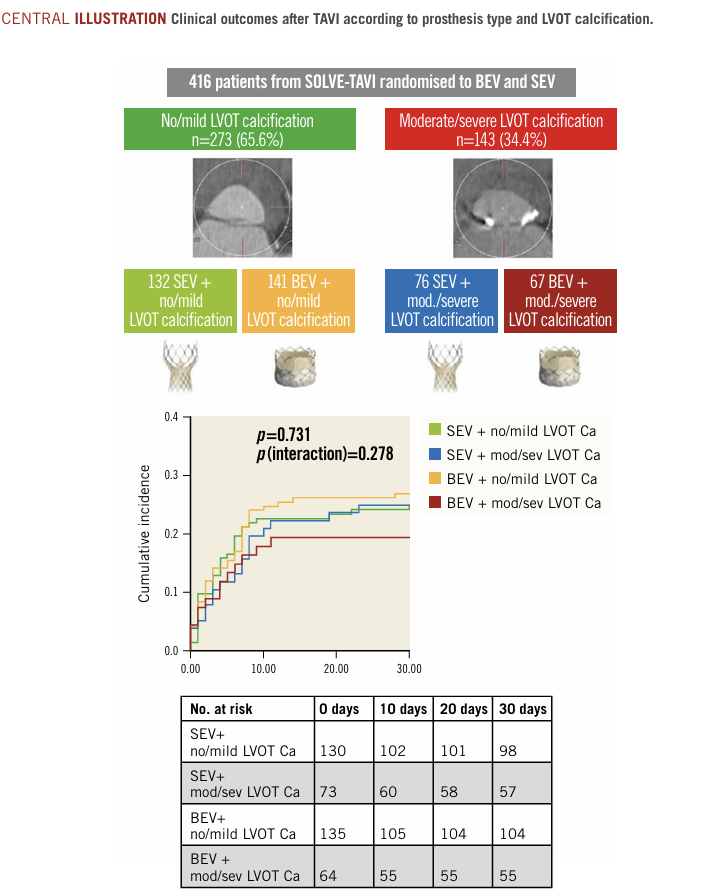
\includegraphics[width=\linewidth]{images/tavi/fig TAVI LVOT calcification.png}
  \caption{嚴重的環下區域及左心室流出道（LVOT）鈣化。多層電腦斷層掃描（MDCT）的橫向軸位與斜矢狀影像顯示，接受經導管主動脈瓣置換（TAVI）評估的患者在環下區域和LVOT有中度至重度鈣化。上排：左冠狀動脈瓣下方的環下區域及LVOT有中度鈣化。下排：左冠狀動脈瓣下方的環下區域及LVOT有重度鈣化，並延伸至右冠狀動脈瓣區域。中度及/或重度鈣化的存在（箭頭所示）可能導致與其他條件相同的患者相比，主動脈根部破裂的風險增加。縮寫：AO 為主動脈，LA 為左心房，LV 為左心室，RA 為右心房，RV 為右心室。\cite{Soon2017}}
  \label{images/tavi/fig TAVI LVOT calcification}
\end{marginfigure}
% \cite{Soon2017}
% from paper:  Multimodality Imaging for Planning and Follow-up of Transcatheter Aortic Valve Replacement

\subsection{LVOT calcium grading}
\caption{LVOT calcium grading definitions. 請參考 Figure ~\ref{images/tavi/fig TAVI LVOT calcification}.}
\begin{longtable}{p{2cm} p{7cm}}
\hline
\textbf{分類} & \textbf{定義} \\ \hline
\endfirsthead
\hline
\textbf{分類} & \textbf{定義} \\ \hline
\endhead
\hline
\endfoot
無（None） & 無鈣化 \\ \hline
輕度（Mild） & 出現 1 個鈣化結節，且任一方向延伸 < 5 毫米，覆蓋左心室流出道（LVOT）周邊 < 10\%。 \\ \hline
中度（Moderate） & 出現 2 個鈣化結節，或 1 個鈣化結節任一方向延伸 > 5 毫米，或覆蓋 LVOT 周邊 > 10\%。 \\ \hline
重度（Severe） & 出現多個鈣化結節，或單個焦點的鈣化結節延伸 > 10 毫米，或覆蓋 LVOT 周邊 > 20\%。 \\ \hline
\end{longtable}

\begin{figure}
    \centering
    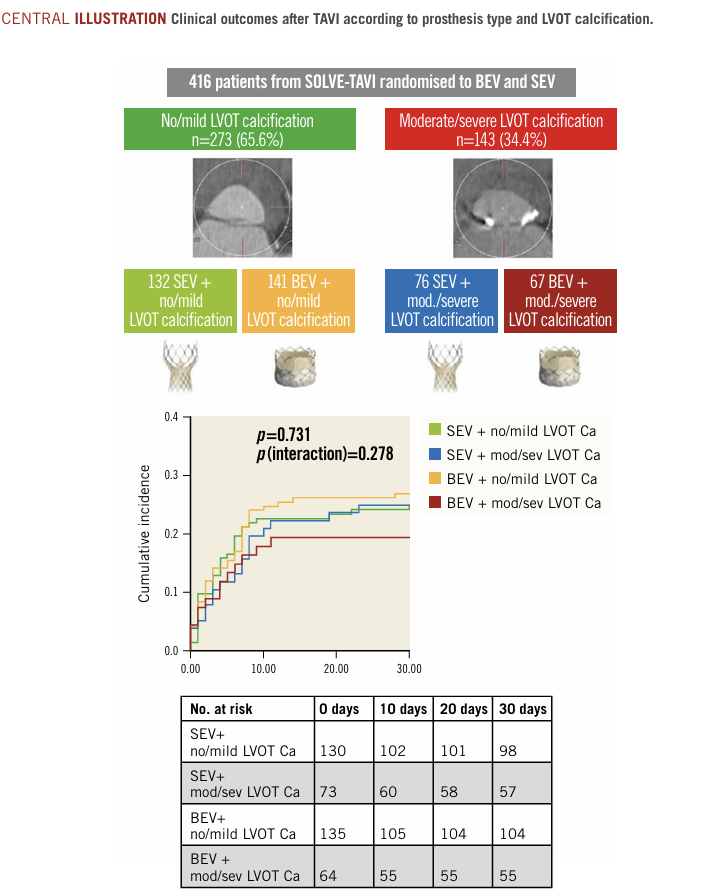
\includegraphics[width=1.0\linewidth]{images/tavi/fig TAVI LVOT calcification.png}
    \caption{LVOT calcification was analyzed in 416 patients from the SOLVE-TAVI trial, which randomized patients to TAVI with either BEV or SEV and either general anesthesia or conscious sedation. There was no significant difference in the incidence of a composite endpoint of all-cause mortality, stroke, moderate or severe paravalvular regurgitation, permanent pacemaker implantation and annulus rupture. There was no interaction between prosthesis type and LVOT calcification. BEV: balloon-expandable valve; Ca: calcification; LVOT: left ventricular outflow tract; SEV: self-expanding valve; TAVI: transcatheter aortic valve implantation.\cite{Farhan2022}}
    \label{images/tavi/fig TAVI LVOT calcification}
\end{figure}
%Impact of moderate or severe left ventricular outflow tract calcification on clinical outcomes of patients with severe aortic stenosis undergoing transcatheter aortic valve implantation with self- and balloon-expandable valves: a post hoc analysis from the SOLVE-TAVI trial. S. Farhan, G. Stachel, S. Desch, T. Kurz, H. J. Feistritzer, P. Hartung, et al. EuroIntervention 2022 Vol. 18 Issue 9 Pages 759-768. Accession Number: 35942626 PMCID: PMC11064680 DOI: 10.4244/EIJ-D-22-00156



\section{How to enter LV efficiently?}
在執行TAVI時，最基本的工夫就是要能夠通過狹窄的主動脈瓣，進入到LV cavity. Dr. Elias Hanna在YouTube上推出了非常詳細的影片，值得大家參考。我是在Mainz進修時，與Dr. Kabir認識，他跟我推薦我才知道網路上有這麼詳細的教學資料。

\begin{figure}
%\vskip -1.2in
    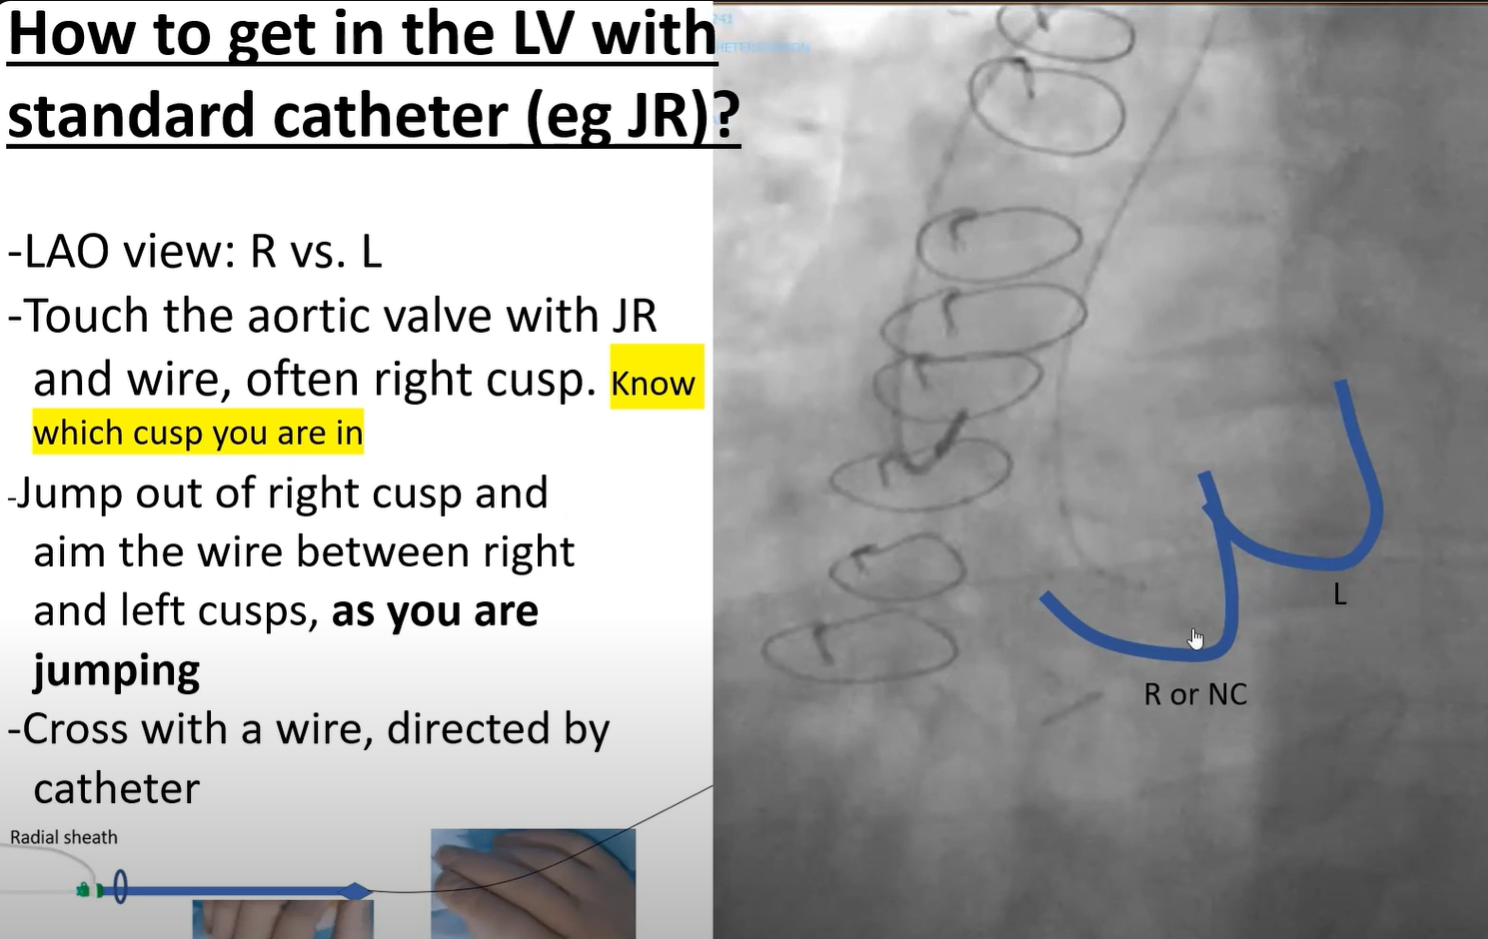
\includegraphics{images/teer/fig Elias Hanna teaching.png}
    \caption{網路上search keywords: \href{https://www.youtube.com/watch?v=P0czcxqgfOo}{Elias Hanna} Left Ventricular catheterization. \href{https://www.youtube.com/watch?v=P0czcxqgfOo}{\textbf{點擊這裡可以連至YouTube}}}
    \label{images/teer/fig Elias Hanna teaching}
\end{figure}


\section{THV implantation technique}
\begin{figure}
    \centering
    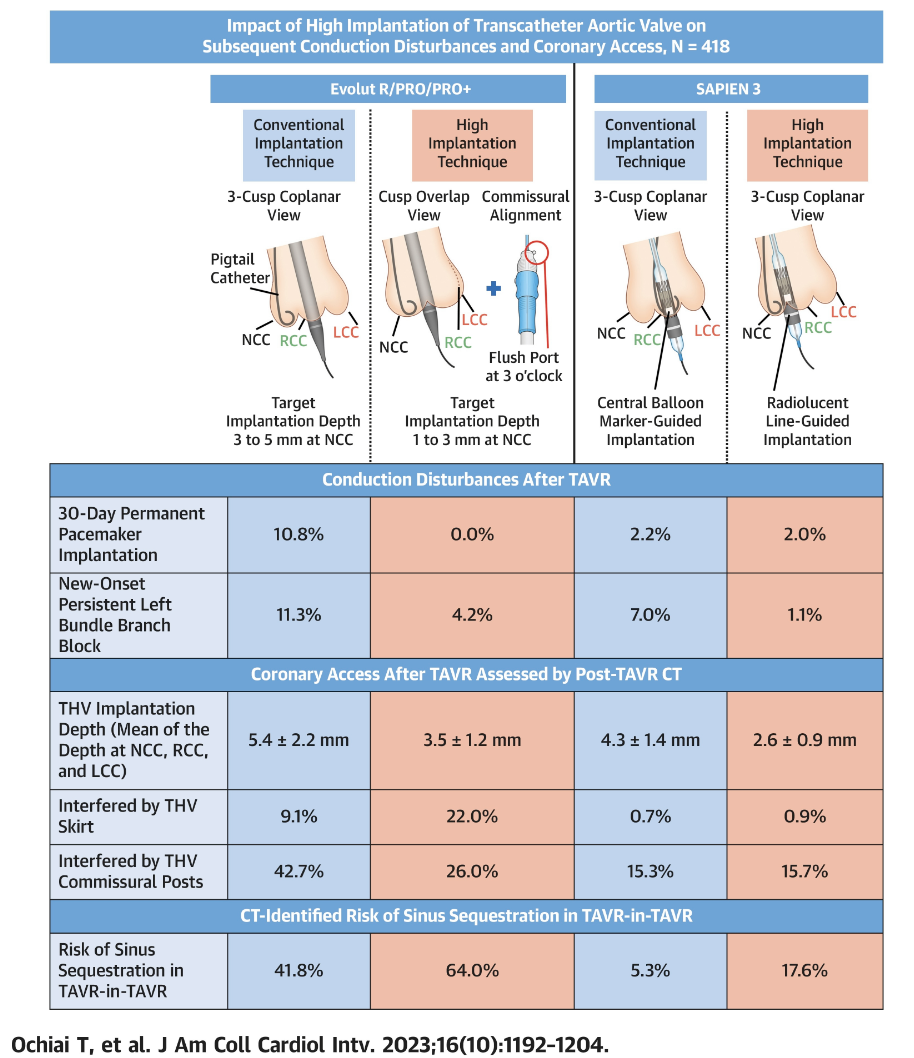
\includegraphics[width=1.0\linewidth]{images/tavi/fig TAVI implantation tech.png}
    \caption{高位植入 (high implantation) 經導管心臟瓣膜（THV）可顯著減少 TAVI（經導管主動脈瓣置換術）後的傳導異常。然而，TAVI 後的電腦斷層掃描顯示，TAVI 後未來可能會面臨不利的冠狀動脈通路風險，以及在 TAVI 疊加 TAVI 時發生竇房分離的風險。\cite{Ochiai2023}}
    \label{images/tavi/fig TAVI implantation tech}
\end{figure}


\section{Step-by-Step of TAVI}
在選擇合適的患者和瓣膜後，手術分為五個連續的步驟：血管通路、穿越瓣膜、氣囊主動脈瓣成形術（BAV）、瓣膜植入和通路閉合。


\begin{longtable}{p{1cm} p{9cm}}
\caption{TAVI手術流程}
\hline
\textbf{步驟} & \textbf{說明} \\ \hline
\endfirsthead
\hline
\textbf{步驟} & \textbf{說明} \\ \hline
\endhead
\hline
\endfoot
1 & 使用 3D CT 和超音波確認經導管心臟瓣膜（THV）大小。 \\ \hline
2 & 確認 THV 的置入側，即右或左股動脈。 \\ \hline
3 & 確認血管通路。 \\ \hline
4 & 放置並確認經靜脈的右心室起搏導管。 \\ \hline
5 & 套管插入（sheath insertion）。 \\ \hline
6 & 在非冠狀動脈瓣葉處置入診斷用豬尾導管。 \\ \hline
7 & 建立共面視角（co-planar view）。 \\ \hline
8 & 穿越原生瓣膜。 \\ \hline
9 & 測量血流動力學。 \\ \hline
10 & 進行 THV 定位。 \\ \hline
11 & 部分部署（for Self-expanding THV: 在部署 2/3 時評估位置）。 \\ \hline
12 & 完全部署 THV。 \\ \hline
13 & 通過血流動力學、超音波和動脈造影評估 THV 部署後的效果。 \\ \hline
14 & 移除設備和套管。 \\ \hline
15 & 血管閉合。 \\ \hline
\end{longtable}

TAVI時，還需考慮麻醉方式的選擇（局部麻醉加鎮靜劑或全身麻醉）以及在右心室放置臨時起搏導線。在Mainz大多數的TAVI手術使用清醒鎮靜 (conscious sedation)進行，但對全身麻醉的使用也較為靈活。進行全身麻醉的情況下，患者通常會在離開手術室前拔除氣管插管。

對全身麻醉的使用也較為靈活: Mainz的導管室裡，都是single plane Philips導管機。因為是單一球管，所以在病患頭側的空間很大，常規就是麻醉科工作的區域，再加上有透明的鉛屏風防護，所以進行導管瓣膜性心臟病治療時，從頭到尾都有一名麻醉科醫師在病患頭端待命，可以隨時進行插管或藥物給予。

以下為步驟順序。

\subsection{Sizing issue}
治療前，要使用3D CT確認經導管心臟瓣膜（THV）的大小該如何選擇。

THV (transcatheter human valve) 瓣膜尺寸的選擇至關重要，3D成像是關鍵，而3D CTA是最常用的方式。
CT annular diameter 的測量是基於 perimeter (周長)衍生的直徑。
如果直徑介於兩種瓣膜尺寸之間，且竇部 (sinus of Valsalva SOV) 寬度足夠，則考慮選擇較大的瓣膜尺寸。

\begin{longtable}{p{3cm} p{7cm}}
\caption{Sizing issues for TAVI}\\
\hline
\textbf{Parameter} & \textbf{Clinical relevance} \\
\hline
\endfirsthead
\multicolumn{2}{l}{\textit{接續上一頁}} \\
\hline
\textbf{項目} & \textbf{內容} \\
\hline
\endhead
\hline \multicolumn{2}{r}{\textit{接續下一頁}} \\
\endfoot
\endlastfoot

\textbf{Annular diameters} & 
Annular diameter at systole 為主要參數，以此決定THV的大小。保守起見，都用 minimal annular diameter選是最安全的。另一個是依照 average annular diameter來選擇合適的人工瓣膜大小。
\\ \hline

\textbf{LVOT} & 
要特別看有沒有LVOT鈣化。這個與 LVOT or annulus rupture有關。
\\ \hline

\textbf{SoV, sinus of Valsalva} &
SoV diameter都應該要超過28 mm. 
\\ \hline

\textbf{Coronary height} &
這個直接與冠狀動脈 ostium 閉鎖有關。
Coronary artery ostium height: 只的是由NCC往coronary artery ostium inner border的距離。
coronary height should > 10 mm, best should > 12 mm. 
\\ \hline

\end{longtable}


\subsection{Access}
Operator 必須熟練掌握外周血管電腦斷層血管造影（CTA）的影像判讀，以評估所需的外周動脈的大小和品質，以確保順利取得血管通路. 
所有血管通路，都是在血管超音波的引導下進行血管穿刺. 
首先穿刺 RFA, 先將 6 Fr 10 cm sheath 置入後, 用 ProStyle 先植入一組縫合線後，再將 6 Fr sheath 換成 9 Fr sheath. 
另外以 Rt radial artery 為第二條通路 (專門用來將 5-6 Fr pig-tail 置放在 aortic root).

接著靜脈注射 heparin，以達到 ACT> 250秒。保持J型導線作為動脈的進入通路。J型導線隨後更換為較硬的Amplatz Super Stiff（Boston Scientific）導線。瓣膜的傳送套管 introducer sheath 則經此硬導線在透視下導入，以確保順利穿過動脈腔。一旦大套管固定到位後，會檢查核對清單，以確保所有重要步驟已完成，並確保團隊協調和準備好部署瓣膜。


接著，通過6 Fr 10公分的 RRA (Rt radial artery) 通路置入5-6 Fr pig-tail，並將其放置於 non-coronary cusp (非冠狀瓣葉的基底部)。

接著進行一系列主動脈造影，通常在 rapid RV-pacing (快速右心室起搏)的情況下，使用稀釋對比劑來確保充分的影像顯示，在從CTA確定的植入角度下，驗證三個瓣葉的線性對齊（co-planar view）。

\subsection{Valve Crossing and Balloon Aortic Valvuloplasty}
在 Mainz 都是用 6-Fr AL1導管沿著 150公分、0.035英寸的J型導線穿過瓣膜傳送套管，並更換為 straight-tip wire 以穿過瓣膜。通常這個動作都是在透視的左前斜位（LAO）投影下進行 valve crossing, 因為這樣可以在嘗試穿過狹窄的主動脈瓣時，及早發現導線意外進入左主冠狀動脈。

如果無法成功穿越，則將導管更換為 AR1 或 JR4 導管。

成功穿越後，將 straight-tip 導線更換為300公分長的J型導線，然後移除 AL1 導管，並更換為 6 Fr pig-tail catheter。接著，將兩個導管連接到壓力計，並測量左心室和主動脈的收縮壓和舒張壓。

這個時候，都會關注左心室和主動脈的收縮峰值之間的間隔差距（peak-to-peak systolic separation），這是瓣膜狹窄的重要指標，但也應關注左心室和主動脈的舒張末期壓差 (diastolic bloos pressure difference)，這項測量對於評估瓣膜植入後的瓣周漏 (paravalvular leak) 極為重要。

接著，通過彎曲豬尾導管將預成形的硬導線（如Safari2/Boston Scientific, Confida Brecker/Medtronic, Lunderquist/Cook Medical）放置於左心室內，並將導線的 transition point 保持在心尖上方，避免接觸心室壁。

在瓣膜植入期間，嚴密透視監測左心室內的導線位置。

在進行氣囊主動脈瓣成形術（BAV）之前，應在透視（每秒30幀的高解析度電影模式）下檢查 loaded 的 THV delivery system, 以確保其正確裝載。

將系統保持在沖洗口指向側面的方向，檢視葉片是否正確嵌入囊袋內，並向任一方向旋轉幾度，直到能同時看到兩側葉片。植入前的BAV通常在快速右心室起搏的情況下進行，氣囊尺寸基於主動脈瓣環的最小直徑選擇。

\subsection{Valve Implantation}
將瓣膜傳送系統裝載到導線上，進入身體時，要使沖洗口朝上。在透視引導下，將系統沿著導線推進到主動脈瓣annulus. 通常，系統在推進過程中會自動適應 (adjust)到病人的anatomy. 然而，在推進過程中必須隨時監測系統的capsule和 cone, 以確保整個 system 安全通過解剖部位。在解剖結構彎曲較大或鈣化嚴重的情況下，系統在轉彎時可能會在cone和capsule之間產生間隙。此時切勿強行推進系統，以免對患者造成損傷；而是更換為更硬的導線（如Lunderquist/Cook）來協助系統順利轉彎。

當瓣膜傳送系統達到合適的植入位置（目標植入深度為: 3-5 mm）時，應獲得 co-planar 共面影像投影，系統應自然在主動脈瓣環內自我對齊，並與主動脈弓頂部 (aortic arch)保持接觸，以獲得最大穩定性。

\subsection{Self-expandable THV}
透過緩慢的逆時針旋轉推進器來部署生物瓣膜的前1/3，旋轉時按照箭頭標記的方向，以短小的增量進行。約兩圈後，套囊的反應會達到1:1。部署過程中全程在透視下監測瓣膜位置，並根據需要進行位置調整，直到與瓣環接觸為止。套囊具有展開功能，可以在部署過程中使瓣膜自我對齊。對於有主動脈閉鎖不全、高血壓或大瓣環的患者，在部署過程中可考慮使用控制性起搏（90-130次/分鐘）。

如果操作者對瓣膜在瓣環接觸的定位滿意，則繼續部署瓣膜，直到接近「無法回收點」之前。操作者必須在血壓下降時意識到需要快速完成部署，因為隨著瓣膜展開，主動脈瓣結構暫時被阻塞，導致心輸出量暫時消失。系統中設有一種觸覺指示器（「顫動帶」），用於提示套囊接近「無法回收點」。

操作者必須持續旋轉部署旋鈕，直到血壓恢復，但需確保不超過「無法回收點」。當血壓恢復且部署達到約80\%時，應調整影像投影，以消除瓣膜流入處的視差，並透過血管造影和超音波檢查確認瓣膜位置。如果植入團隊對瓣膜的位置和性能感到滿意，則在完全部署前釋放系統的張力，以減少瓣膜移動的可能性。此過程包括將導線稍微回收、輕微向前推送傳送系統，並緩慢轉動部署旋鈕，使葉片逐一分離。在透視下確認框架葉片分離，並確保錐頭居中後，方可將設備取出。

\subsection{balloon-expandable THV}
在Mainz的balloon-expandable THV使用大宗是Sapien 3/Ultra. 置放時採取的策略都是high implantation technique.\cite{Ochiai2023} 置放會採取高位置放，目地是降低傳導問題的發生，並減少永久性節律器置放的需求。

\subsection{Retrieval}

在將瓣膜傳送系統撤回至降主動脈之前，需確認導管尖端與生物瓣膜的流入部分同軸。系統在降主動脈中被鎖定，透過啟動部署旋鈕的觸發器並將灰色手柄收回至藍色部署旋鈕（「灰對藍」）的位置。系統經由硬導線取出，同時保持導線位置於左心室腔中，並重新放置彎曲豬尾導管於左心室內。接著進行同步壓力描記，重點觀察左心室與主動脈壓力描記的舒張期間隔。最後，將彎曲豬尾導管拉回後進行最終血管造影，以評估瓣膜位置和瓣周漏情況。此外，還可以進行經胸或經食道超音波檢查，以在手術結束前再次確認瓣膜位置。

\subsection{Vascular closure}

接著，大套管經由J型導線移除，佈署ProStyle縫合裝置，並注射魚精蛋白中和肝素。ProStyle使用後，再追加6 Fr or 8 Fr的AngioSeal以完成止血。

如果達到滿意的止血效果 (ProStyle x1 + AngioSeal x1之後)，便可移除導線；若未能達到，則可使用額外的ProGlide®或Angio-Seal（Terumo Interventional Systems, Terumo Medical Corporation, Somerset, NJ）血管閉合裝置。通常會透過替代通路進行周邊血管造影，以確保大套管進入處的血管完整性。替代通路的閉合也使用ProGlide或Angio-Seal血管閉合裝置完成。

\subsection{Transcatheter Human Valves}
THV = Transcatheter Human Valves.


\section{Procedure arrangements}
\subsection{Tips and tricks}
\begin{enumerate}
    \item 直接從Rt radial artery (RRA) 穿刺，並經 RRA置放pig-tail在ascending aorta (AsAo), 在手術最後再重新將 RRA pig-tail擺放到 descending abdominal aorta, 就可以完成 RFA 的穿刺部位血管攝影，一氣呵成。
\end{enumerate}

\subsection{Treatment protocol}

\begin{longtable}{p{4cm} p{9cm}}
\caption{Device list for TAVI}\\
\hline
\textbf{項目} & \textbf{內容} \\
\hline
\endfirsthead
\multicolumn{2}{l}{\textit{接續上一頁}} \\
\hline
\textbf{項目} & \textbf{內容} \\
\hline
\endhead
\hline \multicolumn{2}{r}{\textit{接續下一頁}} \\
\endfoot
\endlastfoot

\textbf{導引鞘 (sheaths)} & 
\begin{itemize}
    \item 6 Fr sheats x2 (第一支先進 Rt CFA, 第二支去 Rt radial artery).
    \item 9 Fr 則是接在6 Fr後去 Rt CFA.
    \item TPM sheath: Rt CFV則要再擺一支 TPM sheath.
\end{itemize}
\\ \hline

\textbf{導管 (catheters)} & 
\begin{itemize}
    \item Pig-tail catheters, 6 Fr x2
    \item AL1 catheter, 6 Fr
\end{itemize}
\\ \hline

\textbf{導絲 (wires)} & 
\begin{itemize}
    \item J-tip wire
    \item Safair XS
    \item Terumo GlideWire straight tip
\end{itemize}
\\ \hline

\textbf{急救與麻醉設備} & 
\begin{itemize}
    \item 麻醉機一台，直接擺在病人頭端。
    \item Dl shock 電擊器一台。
\end{itemize}
\\ \hline

\textbf{超音波} & 
Philips EPIC 一台，配備 linear probe, sector probe各一。直接擺在病患頭端。
\\ \hline

\textbf{人工瓣膜 (trancathter human valve, THV} & 
\begin{itemize}
    \item Evolute Fx+
    \item Sapien 3
\end{itemize}
\\ \hline


\end{longtable}


\section{Low-flow and low-gradient severe AS}
Use dimentionless index進行測量: \[ \frac{VTI_{LVOT}}{VTI_{Ao}} \], 若是 \[ \frac{VTI_{LVOT}}{VTI_{Ao}} < 0.25  \] 那就該考慮病人的診斷是否有可能為: low-pressure, low-gradient severe AS. 

\subsection{MDCT and aortic valve calcium score}
雖然Doppler echocardiography是評估主動脈狹窄 (AS)嚴重程度的首選方法，但在部分無法獲得確定性結果的患者中，使用多層電腦斷層掃描（MDCT）衍生的主動脈瓣鈣化 (aortic valve calcium, AVC) 得分可以作為有效的替代工具。這是基於鈣質在主動脈狹窄的發病及進展過程中的基本作用，且其評估不依賴血流相關的指標。

AVC 通過 MDCT 掃描取得的影像進行測量，使用modified Agatston 方法，鈣化的定義為密度超過 130 Hounsfield 單位的連續四個像素。在 AS 的解剖嚴重程度方面，AVC 評估具有良好的相關性，可用來反映血流動力學的嚴重程度。

在傳統的低流量、低梯度 AS 中，區分真性重度與假性重度可以使用負荷劑量超音波（DSE），若患者具有顯著的血流儲備。然而，若無此儲備情況，較高的 AVC 得分可能有助於識別真性重度 AS。在paradoxial low-flow, low-gradient (矛盾性低流量、低梯度) AS 或normal-flow, low gradient (正常流量、低梯度) AS 患者中，若 DSE 不適用或無法提供確定性結果，高 AVC 得分亦可能協助診斷重度 AS。

重度 AS 的 AVC 評分標準為：男性大於 2000 Agatston 單位，女性大於 1200 Agatston 單位。

簡而言之，若是超音波診斷 severe AS碰到困難，可以依據 AVC score來作進一步評估判斷。

% reference: Multimodality Imaging for Planning and Follow-up of Transcatheter Aortic Valve Replacement, reference: 15, 16, 17

\section{Choice between different THV in TAVI procedures}
幾個重點，是我在Mainz這三個月與heart team一起討論時學到的。
\begin{enumerate}
    \item Durability: 應考慮病人的年紀，若是已經80-90歲的病患，在THV的選擇上較不用考慮durability, 以procedure安全為主要考量。但是對於60多歲的病患，因為考慮未來還有20年以上的survival, 就會考慮durability較佳的THV. 例如: 在2024-11的資料看來: durability for Sapine 3 is better then Evolute. 所以2024-11-12 Case 22治療時選的就是Sapien 3 (病患年紀 62歲, Dx: bisucpid AS).
    \item 嚴重的環下鈣化 (LVOT calcificatoin) 以及因此帶來的環破裂 (annular rupture) 風險可能促使選擇使用self-expandable THV. 
    \item 而較短的膜性中隔 (short membranous septum) 則可能增加AV block的風險，因此植入者可能會選擇較短的balloon-expandable THV，以減少壓迫His bundle的可能性
    \item 為了減少發生AV block的風險，對於membranous septum很短的病人，考慮不要用self-expandable THV, 以免要再進行post-dilate導致AV block. 
\end{enumerate}


\section{Post-TAVI imaging follow-up}
在TAVI術後，影像上的追蹤會使用MDCT以及echo.\cite{Soon2017} 

超音波對於追蹤很重要，要看的有下面的重點:
(1) 評估瓣膜支架的 2D 影像，以及瓣膜葉片的形態和活動性；
(2) 測量瓣膜跨植入物的壓力梯度、瓣膜有效開口面積（EOA）及都卜勒速度指數（DVI）；
(3) 評估主動脈逆流的位置（瓣周性或中心性）及其嚴重程度；以及 
(4) 評估左心室的大小和收縮功能，並計算收縮期肺動脈壓。



\begin{figure}
\vskip -1.2in
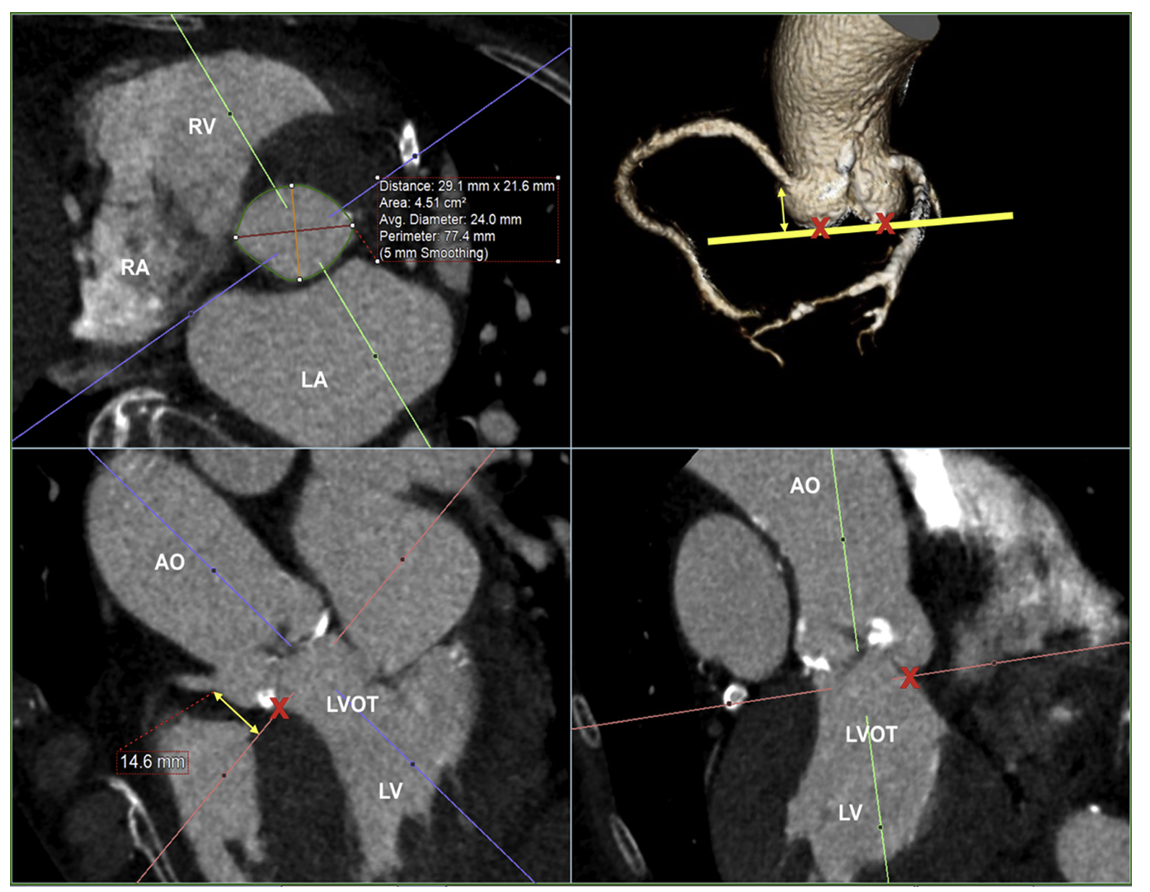
\includegraphics{images/tavi/fig TAVI MDCT.png}
\caption{使用MDCT進行TAVI術後追蹤，主要是觀察各項THV結構。}
\end{figure}

\begin{longtable}{p{3cm} p{9cm}}
\caption{TAVI術後心臟超音波追蹤重點}\\
\hline
\textbf{項目} & \textbf{內容} \\
\hline
\endfirsthead
\multicolumn{2}{l}{\textit{接續上一頁}} \\
\hline
\textbf{項目} & \textbf{內容} \\
\hline
\endhead
\hline \multicolumn{2}{r}{\textit{接續下一頁}} \\
\endfoot
\endlastfoot

\textbf{MDCT after TAVI} & 
\begin{itemize}
    \item THV的結構完整性 (integrity)
    \item 位置 (position)
    \item 貼合度 (apposition)
    \item 圓度 (circularity)
    \item 擴展情況 (expansion)
    \item 瓣周漏 (para-valvular leak)
    \item 併發症 (complications): 血栓 (thrombosis) 和贅生物 (pannus formation)
\end{itemize}
\\ \hline

\textbf{Echocardiography after TAVI} & 
\begin{itemize}
    \item 評估瓣膜支架的 2D 影像，以及瓣膜葉片的形態和活動性
    \item 測量瓣膜跨植入物的壓力梯度、瓣膜有效開口面積（EOA）及都卜勒速度指數
    \item 評估主動脈逆流的位置（瓣周性或中心性）及其嚴重程度
    \item 評估左心室的大小和收縮功能，並計算收縮期肺動脈壓
\end{itemize}
\\ \hline

\textbf{THV stenosis} &
THV stenosis is most often associated with thickening and reduced mobility of the leaflets due to thrombosis, fibrosis, and/or calcification
\\ \hline

\textbf{THV leaflet thickening} & 
Valve leaflet thickening is generally defined as a valve leaflet with thickness $\geq$ 2 mm.
\\ \hline

\textbf{THV thrombosis} &
術後經導管心臟瓣膜葉片增厚在多排電腦斷層掃描（MDCT）中被識別出來。橫軸（左）和斜矢狀面（右）的多排電腦斷層影像顯示在經導管心臟瓣膜葉片上出現局部低密度區域（黃色箭頭），此情況發生於植入後 5 個月，一名 90 歲患者中觀察到此現象。AO，主動脈；LA，左心房；LV，左心室；RA，右心房；RV，右心室。
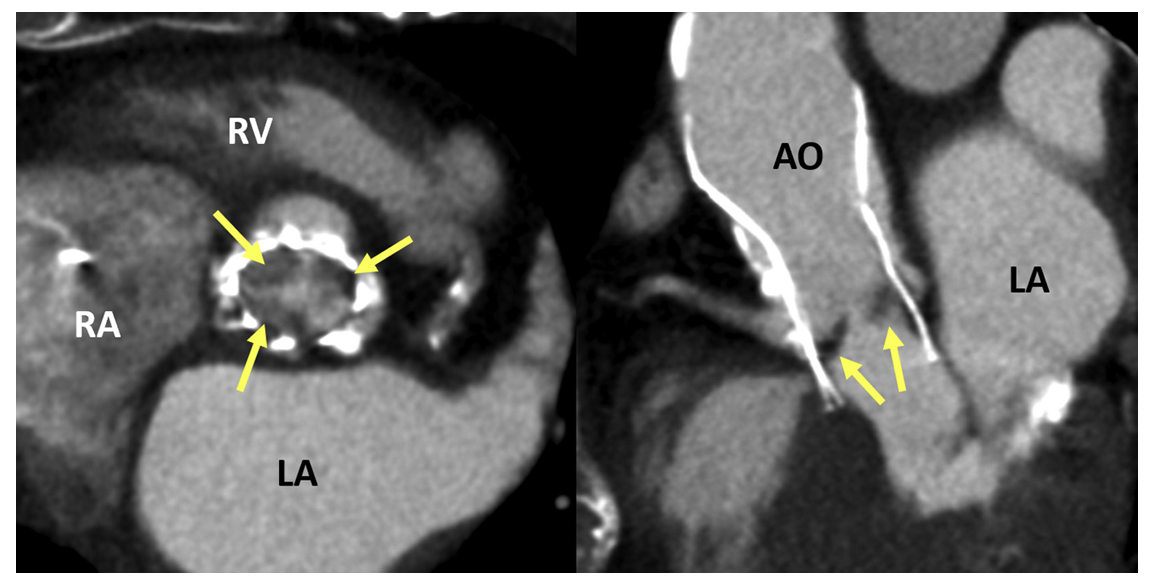
\includegraphics[]{images/tavi/fig TAVI THV thrombosis.png}
\\ \hline

\textbf{Standard method of THV velocity measurement} & 
標準測量方式在 balloon-expandable THV 與 self-expandable THV不同，
經導管主動脈瓣膜面積的測量：(A) 在球囊擴張型經導管心臟瓣膜（THV）中，左心室流出道（LVOT）的直徑（雙黃箭）和速度（黃色圓圈）測量於支架頂端的下方邊緣（紅色虛線）。(B) 在寄生胸長軸放大視圖中測量直徑。在自膨式 THV 中，若 THV 的著陸區位於 LVOT 的較低位置時，直徑和速度可以在支架內進行測量。
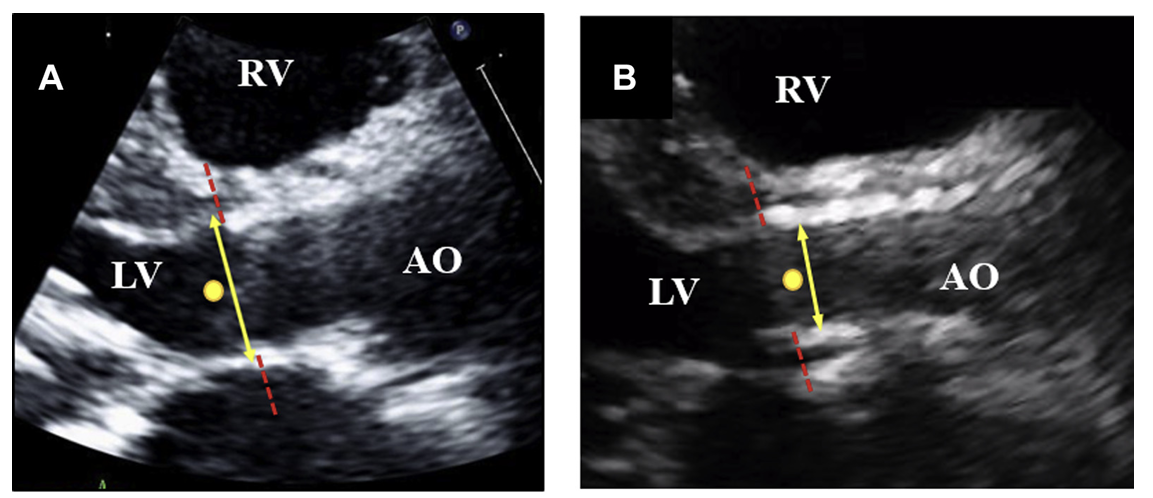
\includegraphics{images/tavi/fig TAVI echo LVOT.png}
\\ \hline
%ref: soon 2017
\end{longtable}

\chapter{TAVI in AR}
在Mainz也見到了TAVI in AR的治療。在過去已經有Jeva Valve的開始，而剛好在2024 ALIGN-AR已經發表。在pivotal study中，technical success成功率達 95\%.\cite{Vahl2024} 

目前AR治療的困境: 外科手術仍然是針對原發性主動脈瓣逆流 (native AR)患者的唯一建議介入治療方法。然而，針對因surgical AVR (surgical aortic valve replacement)而具有高死亡率及併發症風險的患者，目前尚無有效的經導管治療方案。

在pure native AR (純主動脈瓣逆流)的情況下，目前的經導管心臟瓣膜 (THV) 因為沒有像AS那樣有鈣化可以提供THV固著點，所以在native AR嘗試以現有的THV治療，有很高的valve embolization (瓣膜在裝置後就脫離漂移了)及para-valvular leak的風險。 

Trilogy瓣膜是一種經導管心臟瓣膜，由美國研發（JenaValve Technology，美國），目的是為native severe AR的病患提供一種新的治療選擇。

ALIGN-AR 試驗是一項前瞻性、多中心研究，針對中至重度或重度主動脈瓣逆流且不適合手術的患者，使用 Trilogy 經導管心臟瓣膜進行治療。主要目標是評估 30 天內的安全性和 1 年內的療效，並與預設的標準進行比較。

在2018 至 2022 年間，共篩選 346 名患者，最終納入 180 名高風險患者（平均年齡 75.5 歲，女性占 47\%）。技術成功率達 95\%. 30 天內死亡率 2\%, 嚴重中風率 1\%. 該研究之安全性指標均有達成（事件率 27\%，p<0.0001），24\% 的患者需要新植入permanent pacemaker. 1 年內死亡率為 7.8\%（p<0.0001）。

ALIGN-AR研究顯示 Trilogy 經導管瓣膜對不適合手術的主動脈瓣逆流患者具有良好的安全性與療效，短期結果顯示希望，但需進一步長期觀察。\cite{Vahl2024}

\section{TAVI for AR- patient selection}

\begin{longtable}{p{3cm} p{7cm}}
\caption{ALIGN-AR的收案條件概觀}
\hline
\textbf{項目} & \textbf{條件} \\ \hline
\endfirsthead
\hline
\textbf{項目} & \textbf{條件} \\ \hline
\endhead
\hline
\endfoot
\textbf{患者類型} & 有症狀的患者 \\ \hline
\textbf{年齡} & 年滿 18 歲或以上 \\ \hline
\textbf{病情嚴重程度} & 診斷為中度至重度或重度主動脈瓣逆流，表示因主動脈瓣關閉不全，血液從主動脈回流至左心室的情況顯著 \\ \hline
\textbf{手術風險} & 因存在潛在健康問題、年齡較大或其他因素，接受外科主動脈瓣置換術（SAVR）具有較高的死亡風險或併發症風險 \\ \hline
\end{longtable}


\begin{longtable}{p{0.1\textwidth}p{0.9\textwidth}}
\caption{Detailed ALIGN-AR trial patient selection criteria}
\hline
\textbf{Type} & \textbf{Criteria} \\ \hline
\endfirsthead
\hline
\textbf{Type} & \textbf{Criteria (continued)} \\ \hline
\endhead
\hline
\endfoot

% Inclusion Criteria
\multicolumn{2}{l}{\textbf{Inclusion Criteria}} \\ \hline
1 & Adult subjects with severe AR (Grade $\geq$ 3) based on ASE guidelines:
    \begin{itemize}
        \item Jet width $\geq$ 65\% of LVOT.
        \item Vena contracta width $>$ 6 mm.
        \item Holodiastolic flow reversal in the proximal abdominal/descending aorta.
        \item Jet deceleration rate/Pressure half-time $<$ 200 ms.
        \item Regurgitant volume and fraction consistent with Grade 3 or 4 AR thresholds.
    \end{itemize} \\ \hline
2 & Patient symptomatic according to NYHA functional class II or higher. \\ \hline
3 & High surgical risk for SAVR as documented by Heart Team, with agreement that SAVR can be used as a ``bailout''. \\ \hline
4 & Suitable anatomy to accommodate the JenaValve Trilogy\textsuperscript{TM} Heart Valve System. \\ \hline
5 & Written informed consent provided by the patient or legal representative. \\ \hline
6 & Willingness to comply with all post-procedure follow-up requirements. \\ \hline

% Exclusion Criteria
\multicolumn{2}{l}{\textbf{Exclusion Criteria}} \\ \hline
1 & Congenital uni- or bicuspid aortic valve morphology. \\ \hline
2 & Previous prosthetic aortic valve implantation. \\ \hline
3 & Mitral regurgitation $>$ moderate. \\ \hline
4 & Clinically significant CAD requiring revascularization within 30 days before procedure or planned revascularization within 12 months post-procedure. \\ \hline
5 & Echocardiographic evidence of left ventricular thrombus. \\ \hline
6 & Endocarditis within the last 180 days. \\ \hline
7 & Hypertrophic cardiomyopathy with or without obstruction. \\ \hline
8 & Severe pulmonary hypertension (systolic PA pressure $>$ 80 mmHg). \\ \hline
9 & Severe RV dysfunction as assessed clinically and via echocardiography. \\ \hline
10 & Severely reduced LVEF ($<$ 25\%). \\ \hline
11 & Aortic annular perimeter-derived diameter $<$ 21.0 mm or $>$ 28.6 mm, or perimeter $<$ 66 mm or $>$ 90 mm. \\ \hline
12 & Aortic annulus angulation $>$ 70\textdegree. \\ \hline
13 & Straight length of ascending aorta $<$ 55 mm. \\ \hline
14 & Significant disease of ascending aorta (e.g., aneurysm $\geq$ 50 mm or severe atheroma). \\ \hline
15 & Urgent or emergent TAVI required. \\ \hline
16 & Cardiogenic shock or hemodynamic instability requiring inotropic support or ventricular assist device. \\ \hline
17 & Myocardial infarction $<$ 30 days before procedure. \\ \hline
18 & Cerebrovascular event (TIA or stroke) $<$ 180 days before procedure. \\ \hline
19 & Severe renal insufficiency (GFR $<$ 30 ml/min) or recent renal replacement therapy ($<$ 180 days). \\ \hline
20 & Blood dyscrasias (e.g., WBC $<$ 3000/mm$^3$, platelets $<$ 90,000/µl, or anemia [Men: Hgb $<$ 8.1 g/dl; Women: Hgb $<$ 7.4 g/dl]). \\ \hline
21 & Active peptic ulcer or gastrointestinal bleeding $<$ 90 days before procedure. \\ \hline
22 & Known hypersensitivity to aspirin, heparin, ticlopidine, clopidogrel, nitinol, tantalum, or contrast agents. \\ \hline
23 & Contraindication to intraoperative transesophageal echocardiography or MDCT scan. \\ \hline
24 & Estimated life expectancy $<$ 24 months. \\ \hline
25 & Enrollment in another investigational study. \\ \hline
26 & Medical, social, or psychological conditions that preclude participation as per investigator. \\ \hline
27 & Severe dementia impacting consent or compliance with follow-up. \\ \hline
28 & Inability to comply with follow-up requirements. \\ \hline

\end{longtable}


\section{ALIGN-AR trial with focus on Trilogy valve}

\begin{longtable}{p{3cm}p{9cm}}
\caption{Trilogy Valve in ALIGN-AR trial}
\hline
\textbf{項目} & \textbf{內容} \\
\hline
\endfirsthead

\hline
\textbf{項目} & \textbf{內容} \\
\hline
\endhead

\hline
\endfoot

\hline
\textbf{特性} & \\
\hline
結構設計 & 
\begin{itemize}
    \item 使用豬心包膜作為瓣膜材料，並以聚酯縫線固定在自膨脹的鎳鈦合金框架上。
    \item 框架採用冠狀結構設計，能夠壓縮並適配於經導管的置入。
    \item 設計有三個定位定位器（Locators），在展開時與天然瓣膜葉片配對，確保準確定位。
\end{itemize} \\
\hline
防漏功能 & 瓣膜基部有鎳鈦密封環，外覆心包膜裙，用以減少瓣周反流。 \\
\hline
生物相容性與固定性 & 三個定位器捕捉天然瓣膜葉片，並與天然瓣膜小樑解剖學對齊，提供穩定性。 \\
\hline

\textbf{參數} & \\
\hline
適應範圍 & 
\begin{itemize}
    \item 適用於高手術風險的症狀性嚴重主動脈瓣反流患者。
    \item 主動脈瓣直徑必須在 21.0 mm 至 28.6 mm 範圍內，環周長介於 66 mm 至 90 mm。
\end{itemize} \\
\hline
導管系統 & 
\begin{itemize}
    \item 20Fr 引導鞘系統（外徑 22Fr）。
    \item 支持 0.035 英寸導絲。
\end{itemize} \\
\hline
植入技術 & 經股動脈（Transfemoral, TF）途徑進行置入。 \\
\hline

\textbf{置放流程} & \\
\hline
前置準備 & 
\begin{itemize}
    \item 使用 20Fr 的預彎引導鞘將導管系統插入股動脈。
    \item 通過影像學引導（如透視）將導管引導至主動脈瓣位置。
\end{itemize} \\
\hline
定位與對齊 & 
\begin{itemize}
    \item 使用導管系統的 \textbf{Deflector} 機制，將瓣膜的定位器對準天然瓣膜的瓣葉小樑。
    \item 使用 \textbf{Controller} 機制旋轉瓣膜，實現最佳解剖學對齊。
\end{itemize} \\
\hline
定位器展開 & 釋放定位器，使其展開並捕捉天然瓣膜葉片。 \\
\hline
瓣膜部署 & 
\begin{itemize}
    \item 移除導管的安全夾，啟動 \textbf{Deploy} 機制。
    \item 分兩步展開瓣膜：先釋放進口段（密封環），後釋放出口段（眼孔）。
\end{itemize} \\
\hline
確認與完成 & 
\begin{itemize}
    \item 確認瓣膜位置和功能（包括通過超音波評估瓣膜無中重度反流）。
    \item 移除導管系統及引導鞘，完成植入。
\end{itemize} \\
\hline

\end{longtable}




\chapter{致謝}
不到兩個月的時間，參與觀察了共125例經導管瓣膜手術，其中每一例均成功。中間很感謝Mainz Heart Valve Center: Dr. Ralph Stephan von Bardeleben, Dr. Ruf Tobias, Dr. Theresa, Dr. Julian等醫師的指導。也感謝一起受訓的 Dr. Kabir (from India) and Dr. Julian (from Colombia)的一起討論，過程收獲都在滿滿的筆記與這份報告中。希望可以將經驗與技術帶回台灣，並提升在地醫療與研究水平。



我個人也非常享受可以一直作畫筆記的時光 (Figure ~\ref{images/general/fig Mainz notes})。
\begin{figure}
    \centering
    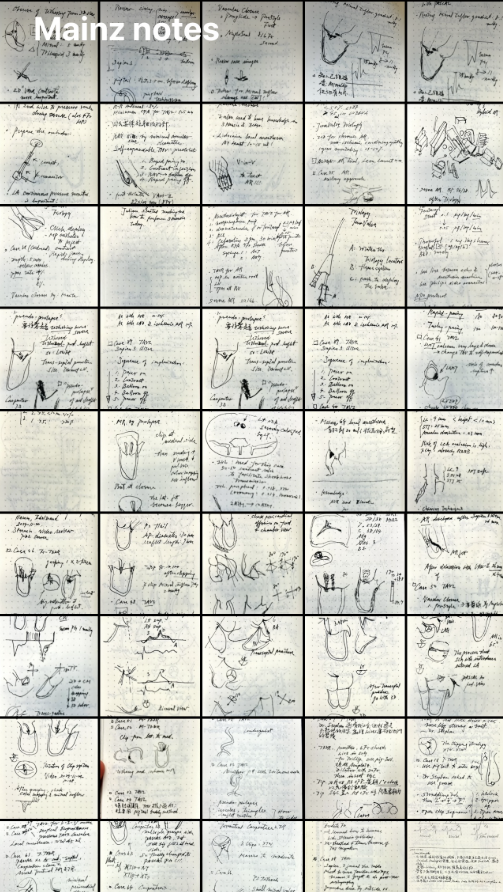
\includegraphics[]{images/general/fig Mainz notes.png}
    \caption{在Mainz Hybrid OR內持續作畫筆記的內容概觀。}
    \label{images/general/fig Mainz notes}
\end{figure}

本報告之citation盡力求完整，並標示清楚quotation/citation/reference. 文件內網路上的影片均有標示。因為病患隱私，所有重要手術均以繪圖方式記錄，若對筆記繪圖有興趣，可以來信 H11135@hch.gov.tw. 

考量檔案內容圖片極多，文件以overleaf製作 (Latex). 文件Latex格式以 Tufte-Book template完成。檔案內容，對於複雜的英文翻譯，以ChatGPT用以下prompt進行: "請幫我翻成繁體中文"，之後再以人工方式確認翻譯內容是否正確。文件中的表格以Latex package: longtable製作，採用ChatGPT輔助加速Latex語法產生 (以下面prompt進行: 請幫我將此表格轉換為latex longtable語法)。

對於文件內容有疑問或指教，歡迎來信: H11135@hch.gov.tw. 
\cite{Adamo2019}

% The bibliography style.
\bibliographystyle{abbrv}
\bibliography{Reference}

\end{document}